% ============================================================
%  يُترجَم بـ XeLaTeX  (في Overleaf: Menu → Compiler → XeLaTeX)
%  الخط: Amiri (متوفر في Overleaf، أو حمّله من github.com/aliftype/amiri)
% ============================================================
\documentclass[12pt,a4paper]{article}
\usepackage[a4paper,margin=1.7cm,top=2.3cm,bottom=2.9cm,headheight=15pt,footskip=1.5cm]{geometry}
\usepackage{amsmath,amssymb}
\usepackage{icomma}
\usepackage[english,bidi=default,layout=lists]{babel}
\babelprovide[import,main]{arabic}
\babelfont{rm}[Scale=1.08]{Amiri}
\babelfont{sf}[Scale=1.08]{Amiri}
\usepackage[most]{tcolorbox}
\usepackage{tikz}
\usetikzlibrary{arrows.meta,calc,shadings}
\usepackage{array}
\usepackage{colortbl}
\usepackage{fancyhdr}
\usepackage{titlesec}
\usepackage{enumitem}
\usepackage{collcell}
\usepackage{needspace}
\usepackage{etoolbox}
\newcolumntype{C}{>{\collectcell\ar}c<{\endcollectcell}}
\pretocmd{\section}{\Needspace{15\baselineskip}}{}{}
\pretocmd{\subsection}{\Needspace{11\baselineskip}}{}{}

\definecolor{cDef}{HTML}{1F4E9C}
\definecolor{cThm}{HTML}{B3261E}
\definecolor{cRem}{HTML}{2E7D32}
\definecolor{cEx}{HTML}{C76B00}
\definecolor{cMeth}{HTML}{6A1B9A}
\definecolor{cSol}{HTML}{00695C}
\definecolor{cSec}{HTML}{1F3A68}

\titleformat{\section}{\Large\bfseries\color{cSec}}{\thesection.}{0.6em}{}[{\color{cSec!60}\titlerule[1pt]}]
\titleformat{\subsection}{\large\bfseries\color{cThm!85!black}}{\thesubsection.}{0.5em}{}
\titlespacing*{\section}{0pt}{14pt}{8pt}
\titlespacing*{\subsection}{0pt}{10pt}{5pt}
\setlength{\parindent}{0pt}
\setlength{\parskip}{4pt}
\setlist{itemsep=2pt,topsep=3pt}

\newtcolorbox{arbox}[3][]{enhanced,
  colback=#2!5,colframe=#2!80!black,arc=2mm,boxrule=0.8pt,
  left=6pt,right=6pt,top=8pt,bottom=5pt,
  fonttitle=\bfseries,coltitle=white,
  title={\foreignlanguage{arabic}{#3}},
  attach boxed title to top right={xshift=-5mm,yshift=-3mm},
  boxed title style={colback=#2!80!black,arc=1.5mm,boxrule=0pt},
  before upper={\selectlanguage{arabic}},
  before skip=8pt,after skip=8pt,breakable,#1}
\newenvironment{BOX}[2]{\begin{otherlanguage}{english}\begin{arbox}{#1}{#2}}{\end{arbox}\end{otherlanguage}}
\newenvironment{tarif}[1][تعريف]{\begin{BOX}{cDef}{#1}}{\end{BOX}}
\newenvironment{khassia}[1][خاصية]{\begin{BOX}{cThm}{#1}}{\end{BOX}}
\newenvironment{molahada}[1][ملاحظة]{\begin{BOX}{cRem}{#1}}{\end{BOX}}
\newenvironment{mithal}[1][مثال]{\begin{BOX}{cEx}{#1}}{\end{BOX}}
\newenvironment{tariqa}[1][طريقة]{\begin{BOX}{cMeth}{#1}}{\end{BOX}}

\newcounter{exo}
\newenvironment{tamrin}[1]{\stepcounter{exo}\begin{BOX}{cSec}{التمرين \theexo: #1}}{\end{BOX}}
\newenvironment{hal}{\Needspace{12\baselineskip}\begin{otherlanguage}{english}\begin{arbox}[breakable]{cSol}{حل التمرين \theexo}}{\end{arbox}\end{otherlanguage}}

\newenvironment{LTR}{\begin{otherlanguage}{english}}{\end{otherlanguage}}
\newcommand{\ar}[1]{\foreignlanguage{arabic}{#1}}

\renewcommand{\dots}{\mathinner{\ldotp\ldotp\ldotp}}
\renewcommand{\ldots}{\mathinner{\ldotp\ldotp\ldotp}}
\renewcommand{\cdots}{\mathinner{\cdotp\cdotp\cdotp}}
\newcommand{\N}{\mathbb{N}}
\newcommand{\Z}{\mathbb{Z}}
\newcommand{\D}{\mathbb{D}}
\newcommand{\Q}{\mathbb{Q}}
\newcommand{\R}{\mathbb{R}}
\newcommand{\pgcd}{\operatorname{PGCD}}
\newcommand{\ppcm}{\operatorname{PPCM}}

% \NLseg{a}{b}{[}{]} ; \NLright{a}{[} ; \NLleft{b}{]}  (interval on a number line)
\newcommand{\NLseg}[4]{\begin{LTR}\begin{tikzpicture}[baseline=-0.6ex]
 \draw[-{Stealth[length=2mm]},gray!70](0,0)--(3.4,0);
 \draw[line width=2pt,cThm!80!black](0.7,0)--(2.7,0);
 \node[cThm!80!black,font=\LARGE] at (0.7,0){$#3$};
 \node[cThm!80!black,font=\LARGE] at (2.7,0){$#4$};
 \node[below=3pt,font=\footnotesize] at (0.7,0){$#1$};
 \node[below=3pt,font=\footnotesize] at (2.7,0){$#2$};
\end{tikzpicture}\end{LTR}}
\newcommand{\NLright}[2]{\begin{LTR}\begin{tikzpicture}[baseline=-0.6ex]
 \draw[-{Stealth[length=2mm]},gray!70](0,0)--(3.4,0);
 \draw[line width=2pt,cThm!80!black](1.3,0)--(3.3,0);
 \node[cThm!80!black,font=\LARGE] at (1.3,0){$#2$};
 \node[below=3pt,font=\footnotesize] at (1.3,0){$#1$};
\end{tikzpicture}\end{LTR}}
\newcommand{\NLleft}[2]{\begin{LTR}\begin{tikzpicture}[baseline=-0.6ex]
 \draw[-{Stealth[length=2mm]},gray!70](0,0)--(3.4,0);
 \draw[line width=2pt,cThm!80!black](0.05,0)--(2.1,0);
 \node[cThm!80!black,font=\LARGE] at (2.1,0){$#2$};
 \node[below=3pt,font=\footnotesize] at (2.1,0){$#1$};
\end{tikzpicture}\end{LTR}}

% ---------- social-media icons (pure TikZ) ----------
\definecolor{cFB}{HTML}{1877F2}
\definecolor{cTG}{HTML}{229ED9}
\definecolor{cIG1}{HTML}{FEDA75}
\definecolor{cIG2}{HTML}{D62976}
\definecolor{cIG3}{HTML}{4F5BD5}
\newcommand{\fbicon}{\begin{LTR}\begin{tikzpicture}[baseline=-0.75ex,x=1em,y=1em]
 \fill[cFB] (0,0) circle (0.55);
 \node[white,inner sep=0,font=\usefont{TU}{lmss}{bx}{n}\small] at (0.04,-0.02) {f};
\end{tikzpicture}\end{LTR}}
\newcommand{\igicon}{\begin{LTR}
\begin{tikzpicture}[baseline=-0.75ex,x=1em,y=1em]
 \shade[lower left=cIG1,lower right=cIG2,upper left=cIG2,upper right=cIG3,rounded corners=0.28em] (-0.55,-0.55) rectangle (0.55,0.55);
 \draw[white,line width=0.09em,rounded corners=0.18em] (-0.36,-0.36) rectangle (0.36,0.36);
 \draw[white,line width=0.09em] (0,0) circle (0.17);
 \fill[white] (0.22,0.22) circle (0.05);
\end{tikzpicture}\end{LTR}}
\newcommand{\tgicon}{\begin{LTR}
\begin{tikzpicture}[baseline=-0.75ex,x=1em,y=1em]
 \fill[cTG] (0,0) circle (0.55);
 \fill[white] (-0.33,0.0) -- (0.32,0.27) -- (0.2,-0.3) -- (0.0,-0.15) -- (-0.08,-0.28) -- (-0.08,-0.08) -- cycle;
 \fill[cTG!70!black] (-0.08,-0.08) -- (0.25,0.2) -- (0.0,-0.15) -- (-0.08,-0.28) -- cycle;
\end{tikzpicture}\end{LTR}}
% page number: black box, white two-digit number, at the right of the social row
\newcommand{\PageBox}{\begin{LTR}\tikz[baseline=(p.base)]\node[fill=black,text=white,inner sep=2.5pt,minimum width=1.6em,minimum height=1.3em,font=\usefont{TU}{lmss}{bx}{n}\small](p){\ifnum\value{page}<10 0\fi\arabic{page}};\end{LTR}}
% visual left-to-right order: Telegram | Instagram | Facebook | page box
\newcommand{\SocialRow}{\begin{otherlanguage}{english}%
 \ar{\textbf{الأستاذ سوايسية هشام للرياضيات}}\ \tgicon\hfill
 \textbf{prof\_hicham\_math}\ \igicon\hfill
 \ar{\textbf{الأستاذ سوايسية هشام للرياضيات}}\ \fbicon\hspace{2.2em}\PageBox\end{otherlanguage}}

\pagestyle{fancy}
\fancyhf{}
\renewcommand{\headrulewidth}{0.6pt}
\renewcommand{\footrulewidth}{0.4pt}
% \SetHeader{right head: document title}{left head: level -- stream}
\newcommand{\SetHeader}[2]{%
 \fancyhead[C]{\parbox{\textwidth}{\ar{#1\hfill #2}}}%
 \fancyfoot[C]{\parbox{\textwidth}{\small\SocialRow}}}
\usepackage{tkz-tab}
\usepackage{multicol}
% variation / sign table (LTR)
\newenvironment{TAB}{\par\begin{center}\begin{LTR}\begin{tikzpicture}[scale=0.95,every node/.style={font=\small}]}{\end{tikzpicture}\end{LTR}\end{center}}
% grid + axes, clipped: \begin{GR}{xmin}{xmax}{ymin}{ymax}{unit cm}
\newenvironment{GR}[5]{\par\begin{center}\begin{LTR}\begin{tikzpicture}[x=#5cm,y=#5cm,font=\footnotesize]
 \draw[gray!25,very thin] (#1,#3) grid (#2,#4);
 \draw[-{Stealth[length=2mm]}] (#1,0)--(#2+0.3,0) node[below left]{$x$};
 \draw[-{Stealth[length=2mm]}] (0,#3)--(0,#4+0.3) node[below left]{$y$};
 \node[below left] at (0,0){$O$};
 \begin{scope}\clip (#1,#3) rectangle (#2,#4);}
{\end{scope}\end{tikzpicture}\end{LTR}\end{center}}
\newcommand{\Ticks}[2]{\foreach \t in {#1} \node[below,font=\scriptsize] at (\t,0){$\t$}; \foreach \t in {#2} \node[left,font=\scriptsize] at (0,\t){$\t$};}
\newcommand{\bx}[1]{\ensuremath{\colorbox{cDef!12}{$\displaystyle #1$}}}
\newcommand{\TwoCol}[4]{\par\begin{LTR}\noindent\begin{minipage}[t]{#1\textwidth}\selectlanguage{arabic}#2\end{minipage}\hfill\begin{minipage}[t]{#3\textwidth}\selectlanguage{arabic}#4\end{minipage}\end{LTR}\par}
\newcommand{\RL}[4]{\TwoCol{#3}{#4}{#1}{#2}}  % \RL{w1}{right content}{w2}{left content}
\newcommand{\ok}{$\textcolor{cRem}{\checkmark}$}
\newcommand{\limn}{\displaystyle\lim_{n\to+\infty}}
% sub-questions, each on its own line
\newenvironment{sq}{\begin{itemize}[leftmargin=2.4em,itemsep=3pt]}{\end{itemize}}
\newcommand{\qa}{\item[(أ)]}\newcommand{\qb}{\item[(ب)]}\newcommand{\qc}{\item[(جـ)]}\newcommand{\qd}{\item[(د)]}\newcommand{\qe}{\item[(هـ)]}
\newcommand{\pa}{\par\smallskip\textbf{(أ)} }\newcommand{\pb}{\par\smallskip\textbf{(ب)} }\newcommand{\pc}{\par\smallskip\textbf{(جـ)} }\newcommand{\pd}{\par\smallskip\textbf{(د)} }\newcommand{\pe}{\par\smallskip\textbf{(هـ)} }
\newcommand{\QQ}[1]{\par\smallskip\textbf{#1.} }
\newenvironment{tmr}{\stepcounter{exo}\begin{BOX}{cSec}{تمرين محلول \theexo}}{\end{BOX}}
\newcommand{\ABC}[3]{\\[2pt]\begin{tabular}{p{0.28\textwidth}p{0.28\textwidth}p{0.28\textwidth}}(جـ) \ #3 & (ب) \ #2 & (أ) \ #1\end{tabular}}
\pretocmd{\section}{\Needspace{24\baselineskip}}{}{}
\newtcbox{\bxtbox}{on line,colback=cDef!12,colframe=cDef!12,boxrule=0pt,arc=1pt,boxsep=0pt,left=2pt,right=2pt,top=1pt,bottom=1pt}
\newcommand{\bxt}[1]{\foreignlanguage{english}{\bxtbox{\ar{#1}}}}
\SetHeader{\small\bfseries\color{cSec}تمارين البكالوريا: النهايات والاستمرارية والاشتقاقية}{\small\color{cSec}السنة الثالثة ثانوي -- الشعب العلمية}
\begin{document}
\begin{LTR}
\begin{tcolorbox}[enhanced,colback=cSec,colframe=cSec,arc=3mm,halign=center,boxrule=0pt,top=12pt,bottom=12pt,before upper={\selectlanguage{arabic}}]
{\color{white}\fontsize{21}{27}\selectfont\bfseries تمارين البكالوريا في النهايات والاستمرارية والاشتقاقية}\\[8pt]
{\color{white}\large مع الحلول المفصلة -- الدوال كثيرات الحدود، الناطقة والصماء}\\[5pt]
{\color{white}\large علوم تجريبية -- تقني رياضي}
\end{tcolorbox}
\end{LTR}

\section{تمارين البكالوريا -- شعبة علوم تجريبية}
% ===================== بكالوريا 2014 -- الموضوع الثاني =====================
\begin{tamrin}{بكالوريا 2014 -- الموضوع الثاني -- علوم تجريبية}
\textbf{I.} لتكن $g$ الدالة العددية المعرفة على $\R$ كما يلي: $g(x)=2x^{3}-4x^{2}+7x-4$.
\QQ{1}
\begin{sq}
\qa احسب $\lim\limits_{x\to-\infty}g(x)$ و $\lim\limits_{x\to+\infty}g(x)$.
\qb ادرس اتجاه تغيّر الدالة $g$ على $\R$ ثم شكّل جدول تغيّراتها.
\end{sq}
\QQ{2}
\begin{sq}
\qa بيّن أن المعادلة $g(x)=0$ تقبل حلا وحيدا $\alpha$ حيث $0{,}7<\alpha<0{,}8$.
\qb استنتج حسب قيم العدد الحقيقي $x$ إشارة $g(x)$.
\end{sq}
\textbf{II.} نعتبر الدالة العددية $f$ المعرفة على $\R$ كما يلي: $f(x)=\dfrac{x^{3}-2x+1}{2x^{2}-2x+1}$، و $(C_f)$ تمثيلها البياني في المستوي المنسوب إلى معلم متعامد ومتجانس $(O;\vec i,\vec j)$.
\QQ{1} احسب $\lim\limits_{x\to-\infty}f(x)$ و $\lim\limits_{x\to+\infty}f(x)$.
\QQ{2}
\begin{sq}
\qa بيّن أنه من أجل كل $x$ من $\R$: $f(x)=\dfrac12(x+1)+\dfrac{1-3x}{2(2x^{2}-2x+1)}$.
\qb استنتج أن المنحنى $(C_f)$ يقبل مستقيما مقاربا مائلا $(\Delta)$ يطلب تعيين معادلة له.
\qc ادرس الوضع النسبي للمنحنى $(C_f)$ و $(\Delta)$.
\end{sq}
\QQ{3}
\begin{sq}
\qa بيّن أنه من أجل كل $x$ من $\R$: $f'(x)=\dfrac{x\,g(x)}{(2x^{2}-2x+1)^{2}}$ حيث $f'$ مشتقة الدالة $f$.
\qb استنتج إشارة $f'(x)$ حسب قيم $x$ ثم شكّل جدول تغيّرات الدالة $f$ (نأخذ $f(\alpha)\approx-0{,}1$).
\end{sq}
\QQ{4} احسب $f(1)$ ثم حل في $\R$ المعادلة $f(x)=0$.
\QQ{5} أنشئ المستقيم $(\Delta)$ والمنحنى $(C_f)$.
\QQ{6} لتكن $h$ الدالة العددية المعرفة على $\R$ بـ: $h(x)=\dfrac{x^{3}-4x^{2}+2x-1}{2x^{2}-2x+1}$، و $(C_h)$ تمثيلها البياني.
\begin{sq}
\qa تحقّق أنه من أجل كل $x$ من $\R$: $h(x)=f(x)-2$.
\qb استنتج أن $(C_h)$ هو صورة $(C_f)$ بتحويل نقطي بسيط يطلب تعيينه، ثم أنشئ $(C_h)$.
\end{sq}
\end{tamrin}

\begin{hal}
\textbf{الجزء الأول:}

\QQ{1}
\pa $g$ دالة كثيرة حدود، فنهايتها عند $\pm\infty$ هي نهاية حدّها الأعلى درجة $2x^{3}$:
\[\bx{\lim_{x\to-\infty}g(x)=\lim_{x\to-\infty}2x^{3}=-\infty}\qquad \bx{\lim_{x\to+\infty}g(x)=\lim_{x\to+\infty}2x^{3}=+\infty}\]
\pb $g$ قابلة للاشتقاق على $\R$، و $g'(x)=6x^{2}-8x+7$.

مميّز ثلاثي الحدود $6x^{2}-8x+7$ هو: $\Delta=(-8)^{2}-4\times6\times7=64-168=-104<0$، إذن $g'(x)$ من إشارة معامل $x^{2}$ أي $6>0$:
$g'(x)>0$ من أجل كل $x\in\R$، ومنه \bxt{$g$ متزايدة تماما على $\R$}.
\begin{TAB}
\tkzTabInit[lgt=2,espcl=4]{$x$/1,$g'(x)$/1,$g(x)$/2}{$-\infty$,$+\infty$}
\tkzTabLine{,+,}
\tkzTabVar{-/$-\infty$,+/$+\infty$}
\end{TAB}

\QQ{2}
\pa \textbf{مبرهنة القيم المتوسطة:} الدالة $g$ مستمرة (كثيرة حدود) ومتزايدة تماما على المجال $[0{,}7;0{,}8]$، و:
\[g(0{,}7)=2(0{,}343)-4(0{,}49)+7(0{,}7)-4=0{,}686-1{,}96+4{,}9-4=-0{,}374<0\]
\[g(0{,}8)=2(0{,}512)-4(0{,}64)+7(0{,}8)-4=1{,}024-2{,}56+5{,}6-4=0{,}064>0\]
بما أن $g(0{,}7)\times g(0{,}8)<0$، فإن المعادلة $g(x)=0$ تقبل حلا وحيدا $\alpha$ في $]0{,}7;0{,}8[$. وبما أن $g$ متزايدة تماما على $\R$ فهذا الحل وحيد في $\R$:
\bx{0{,}7<\alpha<0{,}8} (القيمة المقربة: $\alpha\approx0{,}786$).

\pb $g$ متزايدة تماما على $\R$ و $g(\alpha)=0$، إذن:
\begin{itemize}
\item إذا كان $x<\alpha$ فإن $g(x)<g(\alpha)$ أي $g(x)<0$؛
\item إذا كان $x>\alpha$ فإن $g(x)>0$؛ و $g(\alpha)=0$.
\end{itemize}
\begin{TAB}
\tkzTabInit[lgt=2,espcl=3]{$x$/1,$g(x)$/1}{$-\infty$,$\alpha$,$+\infty$}
\tkzTabLine{,-,z,+,}
\end{TAB}

\textbf{الجزء الثاني:}

\textbf{مجموعة التعريف:} مميّز $2x^{2}-2x+1$ هو $4-8=-4<0$، إذن $2x^{2}-2x+1>0$ من أجل كل $x\in\R$، فالدالة $f$ معرفة على $\R$.

\QQ{1} نهاية دالة ناطقة عند $\pm\infty$ هي نهاية حاصل قسمة الحدين الأعلى درجة:
\[\lim_{x\to-\infty}f(x)=\lim_{x\to-\infty}\frac{x^{3}}{2x^{2}}=\lim_{x\to-\infty}\frac{x}{2}=-\infty\qquad\text{و}\qquad \lim_{x\to+\infty}f(x)=\lim_{x\to+\infty}\frac{x}{2}=+\infty\]
إذن \bx{\lim_{x\to-\infty}f(x)=-\infty} و \bx{\lim_{x\to+\infty}f(x)=+\infty}.

\QQ{2}
\pa ننطلق من الطرف الثاني ونوحّد المقامات:
\begin{align*}
\frac12(x+1)+\frac{1-3x}{2(2x^{2}-2x+1)}&=\frac{(x+1)(2x^{2}-2x+1)+1-3x}{2(2x^{2}-2x+1)}\\
&=\frac{2x^{3}-2x^{2}+x+2x^{2}-2x+1+1-3x}{2(2x^{2}-2x+1)}\\
&=\frac{2x^{3}-4x+2}{2(2x^{2}-2x+1)}=\frac{2(x^{3}-2x+1)}{2(2x^{2}-2x+1)}=f(x)
\end{align*}
\pb $f(x)-\dfrac12(x+1)=\dfrac{1-3x}{2(2x^{2}-2x+1)}$، وبأخذ حاصل قسمة الحدين الأعلى درجة:
\[\lim_{x\to\pm\infty}\left[f(x)-\frac12(x+1)\right]=\lim_{x\to\pm\infty}\frac{-3x}{4x^{2}}=\lim_{x\to\pm\infty}\frac{-3}{4x}=0\]
إذن المستقيم \bx{(\Delta):\ y=\tfrac12x+\tfrac12} مقارب مائل للمنحنى $(C_f)$ بجوار $-\infty$ وبجوار $+\infty$.

\pc ندرس إشارة الفرق $f(x)-y=\dfrac{1-3x}{2(2x^{2}-2x+1)}$. المقام موجب تماما، فالإشارة هي إشارة $1-3x$ التي تنعدم عند $x=\dfrac13$:
\begin{TAB}
\tkzTabInit[lgt=3,espcl=3.4]{$x$/1,$f(x)-y$/1,\ar{الوضع النسبي}/1.2}{$-\infty$,$\frac13$,$+\infty$}
\tkzTabLine{,+,z,-,}
\tkzTabLine{,\text{\ar{$(C_f)$ فوق $(\Delta)$}},t,\text{\ar{$(C_f)$ تحت $(\Delta)$}},}
\end{TAB}
و $(C_f)$ يقطع $(\Delta)$ في النقطة $\left(\tfrac13;\tfrac23\right)$ لأن $\dfrac12\left(\dfrac13+1\right)=\dfrac23$.

\QQ{3}
\pa $f$ قابلة للاشتقاق على $\R$ (دالة ناطقة مقامها لا ينعدم)، و $f=\dfrac{u}{v}$ مع $u=x^{3}-2x+1$، $u'=3x^{2}-2$، $v=2x^{2}-2x+1$، $v'=4x-2$:
\begin{align*}
f'(x)&=\frac{(3x^{2}-2)(2x^{2}-2x+1)-(x^{3}-2x+1)(4x-2)}{(2x^{2}-2x+1)^{2}}\\
&=\frac{(6x^{4}-6x^{3}-x^{2}+4x-2)-(4x^{4}-2x^{3}-8x^{2}+8x-2)}{(2x^{2}-2x+1)^{2}}\\
&=\frac{2x^{4}-4x^{3}+7x^{2}-4x}{(2x^{2}-2x+1)^{2}}=\frac{x\left(2x^{3}-4x^{2}+7x-4\right)}{(2x^{2}-2x+1)^{2}}
\end{align*}
إذن \bx{f'(x)=\dfrac{x\,g(x)}{(2x^{2}-2x+1)^{2}}}.

\pb المقام موجب تماما، فإشارة $f'(x)$ هي إشارة الجداء $x\,g(x)$:
\begin{TAB}
\tkzTabInit[lgt=2,espcl=2.6]{$x$/1,$x$/1,$g(x)$/1,$f'(x)$/1,$f(x)$/2.2}{$-\infty$,$0$,$\alpha$,$+\infty$}
\tkzTabLine{,-,z,+,t,+,}
\tkzTabLine{,-,t,-,z,+,}
\tkzTabLine{,+,z,-,z,+,}
\tkzTabVar{-/$-\infty$,+/$1$,-/$f(\alpha)$,+/$+\infty$}
\end{TAB}
\bxt{$f$ متزايدة تماما على كل من $]-\infty;0]$ و $[\alpha;+\infty[$}، و \bxt{$f$ متناقصة تماما على $[0;\alpha]$}، مع $f(0)=\dfrac11=1$ و $f(\alpha)\approx-0{,}1$.

\QQ{4} $f(1)=\dfrac{1-2+1}{2-2+1}=\dfrac01$، إذن \bx{f(1)=0}.

$f(x)=0\iff x^{3}-2x+1=0$ (المقام لا ينعدم). بما أن $1$ جذر، نحلل بالقسمة على $x-1$:
\[x^{3}-2x+1=(x-1)(x^{2}+x-1)\]
(تحقق: $(x-1)(x^{2}+x-1)=x^{3}+x^{2}-x-x^{2}-x+1=x^{3}-2x+1$).
مميّز $x^{2}+x-1$: $\Delta=1+4=5$، وجذراه $x=\dfrac{-1-\sqrt5}{2}$ و $x=\dfrac{-1+\sqrt5}{2}$. إذن:
\[\bx{S=\left\{\frac{-1-\sqrt5}{2};\ \frac{-1+\sqrt5}{2};\ 1\right\}}\qquad\left(\frac{-1-\sqrt5}{2}\approx-1{,}62;\ \frac{-1+\sqrt5}{2}\approx0{,}62\right)\]
وهذا منسجم مع جدول التغيّرات: جذر في $]-\infty;0[$ وجذران في $]0;+\infty[$ على جانبي $\alpha$.

\QQ{5} \textbf{الإنشاء:} نعتمد: $(\Delta)$ يمر بـ $(-1;0)$ و $(1;1)$؛ الذروتان $(0;1)$ و $(\alpha;f(\alpha))\approx(0{,}79;-0{,}1)$ (مماسان أفقيان)؛ نقاط التقاطع مع محور الفواصل؛ النقطة $\left(\tfrac13;\tfrac23\right)$؛ وبعض القيم: $f(-2)\approx-0{,}23$، $f(-3)=-0{,}8$، $f(2)=1$، $f(3)\approx1{,}69$.

\QQ{6}
\pa من أجل كل $x\in\R$:
\[f(x)-2=\frac{x^{3}-2x+1-2(2x^{2}-2x+1)}{2x^{2}-2x+1}=\frac{x^{3}-4x^{2}+2x-1}{2x^{2}-2x+1}=h(x)\]
\pb $h(x)=f(x)-2$ يعني: $M(x;y)\in(C_f)\iff M'(x;y-2)\in(C_h)$، إذن:
\bxt{$(C_h)$ صورة $(C_f)$ بالانسحاب الذي شعاعه $\vec u=-2\vec j$}، أي $\vec u\,(0;-2)$.
وبالتالي مقارب $(C_h)$ المائل هو $y=\tfrac12x+\tfrac12-2=\tfrac12x-\tfrac32$.
\begin{GR}{-3.5}{4.5}{-5.5}{3.5}{0.9}
\Ticks{-3,-2,-1,1,2,3,4}{-5,-4,-3,-2,-1,1,2,3}
\draw[cThm,dashed,thick,domain=-3.5:4.5] plot(\x,{(\x+1)/2});
\draw[cThm!60,dashed,domain=-3.5:4.5] plot(\x,{(\x+1)/2-2});
\draw[cDef,very thick,domain=-3.5:4.5,samples=200] plot(\x,{(\x*\x*\x-2*\x+1)/(2*\x*\x-2*\x+1)});
\draw[cRem,very thick,domain=-3.5:4.5,samples=200] plot(\x,{(\x*\x*\x-2*\x+1)/(2*\x*\x-2*\x+1)-2});
\draw[-{Stealth[length=2mm]},cEx,thick](2,1)--(2,-1) node[midway,right]{$\vec u$};
\fill(0,1) circle(1.6pt) (0.786,-0.13) circle(1.6pt) (1,0) circle(1.6pt) (-1.618,0) circle(1.6pt) (0.618,0) circle(1.6pt) (0.333,0.667) circle(1.4pt);
\draw[densely dotted](0.786,0)--(0.786,-0.13);
\node[below,font=\scriptsize] at (0.83,-0.15){$\alpha$};
\node[cDef] at (3.4,2.6){$(C_f)$};
\node[cRem] at (2.8,-1.3){$(C_h)$};
\node[cThm,font=\scriptsize] at (-3.1,-0.6){$(\Delta)$};
\end{GR}
\end{hal}

% ===================== بكالوريا 2009 -- الموضوع الأول =====================
\begin{tamrin}{بكالوريا 2009 -- الموضوع الأول -- علوم تجريبية}
\textbf{I.} $f$ دالة معرّفة على المجال $I=]-\infty;-1[\,\cup\,]-1;0]$ بـ: $f(x)=-x+\dfrac{4}{x+1}$، و $(C_f)$ تمثيلها البياني في مستوٍ منسوب إلى معلم متعامد ومتجانس $(O;\vec i,\vec j)$ كما هو مبيّن في الشكل الآتي.
\begin{GR}{-8}{1}{-5.5}{5}{0.6}
\Ticks{-7,-6,-5,-4,-3,-2,-1}{-5,-4,-3,-2,-1,1,2,3,4}
\draw[cThm,very thick,domain=-8:1] plot(\x,{-\x});
\draw[cThm,very thick,dashed](-1,-5.5)--(-1,5);
\draw[black,very thick,domain=-8:-1.15,samples=150] plot(\x,{-\x+4/(\x+1)});
\draw[black,very thick,domain=-0.6:0,samples=60] plot(\x,{-\x+4/(\x+1)});
\end{GR}
\QQ{1}
\begin{sq}
\qa احسب نهايات $f$ عند الحدود المفتوحة لـ $I$.
\qb بقراءة بيانية ودون دراسة اتجاه $f$، شكّل جدول تغيّراتها.
\end{sq}
\QQ{2} $g$ دالة معرّفة على $[0;+\infty[$ بـ: $g(x)=x+\dfrac{4}{x+1}$، و $(C_g)$ تمثيلها البياني.
\begin{sq}
\qa احسب نهاية $g$ عند $+\infty$.
\qb تحقّق من أن $(C_g)$ يقبل مستقيما مقاربا مائلا $(\Delta)$ عند $+\infty$ يطلب تعيين معادلة له.
\qc ادرس تغيّرات $g$.
\end{sq}
\textbf{II.} $k$ دالة معرّفة على $\R-\{-1\}$ بـ: $k(x)=|x|+\dfrac{4}{x+1}$.
\QQ{1}
\begin{sq}
\qa احسب $\lim\limits_{h\to0^{+}}\dfrac{k(h)-k(0)}{h}$ و $\lim\limits_{h\to0^{-}}\dfrac{k(h)-k(0)}{h}$.
\qb ماذا تستنتج؟ أعط تفسيرا هندسيا لهذه النتيجة.
\end{sq}
\QQ{2} اكتب معادلتي نصفي المماسين $(\Delta_1)$ و $(\Delta_2)$ عند النقطة التي فاصلتها $x_0=0$.
\QQ{3} ارسم $(\Delta_1)$ و $(\Delta_2)$ و $(C_k)$.
\end{tamrin}

\begin{hal}
\textbf{الجزء الأول:}

\QQ{1}
\pa الحدود المفتوحة لـ $I$ هي $-\infty$ و $-1$ (من اليسار ومن اليمين)؛ أما $0$ فمغلق و $f(0)=0+\dfrac41=4$.
\begin{itemize}
\item عند $-\infty$: $\lim\limits_{x\to-\infty}(-x)=+\infty$ و $\lim\limits_{x\to-\infty}\dfrac{4}{x+1}=0$، إذن \bx{\lim_{x\to-\infty}f(x)=+\infty}.
\item عند $-1$: $\lim\limits_{x\to-1}(-x)=1$، و $x+1<0$ إذا كان $x<-1$، و $x+1>0$ إذا كان $x>-1$:
\[\lim_{x\to-1^{-}}\frac{4}{x+1}=\frac{4}{0^{-}}=-\infty\qquad \lim_{x\to-1^{+}}\frac{4}{x+1}=\frac{4}{0^{+}}=+\infty\]
إذن \bx{\lim_{x\to-1^{-}}f(x)=-\infty} و \bx{\lim_{x\to-1^{+}}f(x)=+\infty}، والمستقيم $x=-1$ مقارب عمودي لـ $(C_f)$.
\end{itemize}
\pb من الشكل: المنحنى نازل على كل من المجالين، إذن $f$ متناقصة تماما على كل من $]-\infty;-1[$ و $]-1;0]$:
\begin{TAB}
\tkzTabInit[lgt=2,espcl=3]{$x$/1,$f(x)$/2.2}{$-\infty$,$-1$,$0$}
\tkzTabVar{+/$+\infty$,-D+/$-\infty$/$+\infty$,-/$4$}
\end{TAB}
(للتأكد: $f'(x)=-1-\dfrac{4}{(x+1)^{2}}<0$.)

\QQ{2}
\pa $\lim\limits_{x\to+\infty}x=+\infty$ و $\lim\limits_{x\to+\infty}\dfrac{4}{x+1}=0$، إذن \bx{\lim_{x\to+\infty}g(x)=+\infty}.
\pb $g(x)-x=\dfrac{4}{x+1}$ و $\lim\limits_{x\to+\infty}\dfrac{4}{x+1}=0$، إذن المستقيم \bx{(\Delta):\ y=x} مقارب مائل لـ $(C_g)$ عند $+\infty$.
وبما أن $g(x)-x=\dfrac4{x+1}>0$ على $[0;+\infty[$ فإن $(C_g)$ فوق $(\Delta)$.
\pc $g$ قابلة للاشتقاق على $[0;+\infty[$ و:
\[g'(x)=1-\frac{4}{(x+1)^{2}}=\frac{(x+1)^{2}-4}{(x+1)^{2}}=\frac{(x+1-2)(x+1+2)}{(x+1)^{2}}=\frac{(x-1)(x+3)}{(x+1)^{2}}\]
على $[0;+\infty[$: $x+3>0$ و $(x+1)^{2}>0$، فإشارة $g'(x)$ هي إشارة $x-1$. القيم: $g(0)=4$ و $g(1)=1+\dfrac42=3$.
\begin{TAB}
\tkzTabInit[lgt=2,espcl=3]{$x$/1,$g'(x)$/1,$g(x)$/2}{$0$,$1$,$+\infty$}
\tkzTabLine{,-,z,+,}
\tkzTabVar{+/$4$,-/$3$,+/$+\infty$}
\end{TAB}
\bxt{$g$ متناقصة تماما على $[0;1]$ ومتزايدة تماما على $[1;+\infty[$}.

\textbf{الجزء الثاني:}
حسب تعريف القيمة المطلقة: إذا كان $x\geqslant0$ فإن $k(x)=x+\dfrac4{x+1}=g(x)$، وإذا كان $x\leqslant0$ ($x\neq-1$) فإن $k(x)=-x+\dfrac4{x+1}=f(x)$. و $k(0)=4$.

\QQ{1}
\pa من أجل $h>0$:
\[\frac{k(h)-k(0)}{h}=\frac{h+\frac{4}{h+1}-4}{h}=1+\frac{4-4(h+1)}{h(h+1)}=1+\frac{-4h}{h(h+1)}=1-\frac{4}{h+1}\]
إذن \bx{\lim_{h\to0^{+}}\frac{k(h)-k(0)}{h}=1-4=-3}.

من أجل $h<0$ ($h\neq-1$):
\[\frac{k(h)-k(0)}{h}=\frac{-h+\frac{4}{h+1}-4}{h}=-1-\frac{4}{h+1}\]
إذن \bx{\lim_{h\to0^{-}}\frac{k(h)-k(0)}{h}=-1-4=-5}.

\pb النهايتان منتهيتان ومختلفتان ($-3\neq-5$)، إذن:

\bxt{$k$ قابلة للاشتقاق على يمين $0$ وعلى يساره}، لكن:

\bxt{$k$ غير قابلة للاشتقاق عند $0$} ($k'_d(0)=-3$ و $k'_g(0)=-5$).

\textbf{التفسير الهندسي:} المنحنى $(C_k)$ يقبل عند النقطة $A(0;4)$ نصفي مماسين مختلفين في الاتجاه: $A$ \textbf{نقطة زاوية}.

\QQ{2}
\begin{itemize}
\item نصف المماس على اليمين ($x\geqslant0$)، معامل توجيهه $-3$: \bx{(\Delta_1):\ y=-3x+4,\ x\geqslant0}.
\item نصف المماس على اليسار ($x\leqslant0$)، معامل توجيهه $-5$: \bx{(\Delta_2):\ y=-5x+4,\ x\leqslant0}.
\end{itemize}

\QQ{3} $(C_k)$ يتكون من $(C_f)$ (لـ $x\leqslant0$) و $(C_g)$ (لـ $x\geqslant0$). جدول تغيّرات $k$:
\begin{TAB}
\tkzTabInit[lgt=2,espcl=2.4]{$x$/1,$k(x)$/2.2}{$-\infty$,$-1$,$0$,$1$,$+\infty$}
\tkzTabVar{+/$+\infty$,-D+/$-\infty$/$+\infty$,R/,-/$3$,+/$+\infty$}
\tkzTabIma{2}{4}{3}{$4$}
\end{TAB}
المقاربات: $x=-1$ (عمودي)، $y=-x$ بجوار $-\infty$ (لأن $k(x)-(-x)=\dfrac4{x+1}\to0$)، و $y=x$ بجوار $+\infty$.
\begin{GR}{-6}{6}{-5}{9}{0.55}
\Ticks{-5,-4,-3,-2,-1,1,2,3,4,5}{-4,-3,-2,-1,1,2,3,4,5,6,7,8}
\draw[cThm,dashed,thick,] (-6,6)--(-1,1) node[pos=0.12,above right]{$y=-x$};
\draw[cThm,dashed,thick,] (0,0)--(6,6) node[pos=0.72,below right]{$y=x$};
\draw[cThm,dashed,thick](-1,-5)--(-1,9);
\draw[cEx,thick](0,4)--(1.6,-0.8) node[right]{$(\Delta_1)$};
\draw[cEx,thick](0,4)--(-0.95,8.75) node[left]{$(\Delta_2)$};
\draw[cDef,very thick,domain=-6:-1.45,samples=150] plot(\x,{-\x+4/(\x+1)});
\draw[cDef,very thick,domain=-0.6:0,samples=80] plot(\x,{-\x+4/(\x+1)});
\draw[cDef,very thick,domain=0:6,samples=150] plot(\x,{\x+4/(\x+1)});
\fill(0,4) circle(1.8pt) node[above right]{$A$} (1,3) circle(1.6pt) (-3,1) circle(1.4pt);
\node[cDef] at (4.3,7.2){$(C_k)$};
\end{GR}
\end{hal}

% ===================== بكالوريا 2008 -- الموضوع الأول =====================
\begin{tamrin}{بكالوريا 2008 -- الموضوع الأول -- علوم تجريبية}
المنحنى $(C)$ الآتي هو التمثيل البياني للدالة العددية $g$ المعرّفة على $I=]-1;+\infty[$ بـ: $g(x)=x^{3}+3x^{2}+3x-1$.
\begin{GR}{-1.5}{2}{-2.5}{3.5}{1}
\Ticks{-1,1,2}{-2,-1,1,2,3}
\draw[blue,very thick,domain=-1:0.74,samples=100] plot(\x,{\x*\x*\x+3*\x*\x+3*\x-1});
\end{GR}
\QQ{1} بقراءة بيانية:
\begin{sq}
\qa شكّل جدول تغيّرات الدالة $g$ وحدّد $g(0)$ وإشارة $g(0{,}5)$.
\qb علّل وجود عدد حقيقي وحيد $\alpha\in]0;0{,}5[$ يحقق $g(\alpha)=0$.
\qc استنتج إشارة $g(x)$ على المجال $I$.
\end{sq}
\QQ{2} $f$ دالة معرّفة على $]-1;+\infty[$ بـ: $f(x)=\dfrac{x^{3}+3x^{2}+3x+2}{(x+1)^{2}}$، و $(\Gamma)$ تمثيلها البياني.
\begin{sq}
\qa تحقّق أنه من أجل كل $x\in I$: $f'(x)=\dfrac{g(x)}{(x+1)^{3}}$.
\qb عيّن دون حساب $\lim\limits_{x\to\alpha}\dfrac{f(x)-f(\alpha)}{x-\alpha}$ وفسّر النتيجة بيانيا.
\qc جد $\lim\limits_{x\to-1}f(x)$ و $\lim\limits_{x\to+\infty}\left[f(x)-(x+1)\right]$، فسّر النتيجتين بيانيا.
\qd شكّل جدول تغيّرات $f$.
\end{sq}
\QQ{3} نأخذ $\alpha=0{,}26$.
\begin{sq}
\qa عيّن مدوّر $f(\alpha)$ إلى $10^{-2}$.
\qb ارسم المنحنى $(\Gamma)$.
\end{sq}
\end{tamrin}

\begin{hal}
\QQ{1}
\pa من الشكل: المنحنى صاعد على $I$ انطلاقا من النقطة $(-1;-2)$ (مفتوحة)، إذن $g$ متزايدة تماما على $I$؛ ونقرأ $g(0)=-1$ (تقاطع $(C)$ مع محور التراتيب) و $g(0{,}5)>0$ (النقطة ذات الفاصلة $0{,}5$ فوق محور الفواصل).
\begin{TAB}
\tkzTabInit[lgt=2,espcl=3.5]{$x$/1,$g(x)$/2}{$-1$,$+\infty$}
\tkzTabVar{-/$-2$,+/$+\infty$}
\end{TAB}
\bx{g(0)=-1} و \bx{g(0{,}5)>0} (حسابيا: $g(0{,}5)=0{,}125+0{,}75+1{,}5-1=1{,}375$).

\pb $g$ مستمرة (كثيرة حدود) ومتزايدة تماما على $[0;0{,}5]$، و $g(0)=-1<0$ و $g(0{,}5)>0$؛ حسب مبرهنة القيم المتوسطة يوجد عدد حقيقي وحيد $\alpha\in]0;0{,}5[$ يحقق \bx{g(\alpha)=0}.

\pc $g$ متزايدة تماما على $I$ و $g(\alpha)=0$:
\begin{TAB}
\tkzTabInit[lgt=2,espcl=3]{$x$/1,$g(x)$/1}{$-1$,$\alpha$,$+\infty$}
\tkzTabLine{d,-,z,+,}
\end{TAB}
\begin{molahada}
$g(x)=(x+1)^{3}-2$، لأن $(x+1)^{3}=x^{3}+3x^{2}+3x+1$. إذن $g(\alpha)=0\iff(\alpha+1)^{3}=2$، أي $\alpha=\sqrt[3]{2}-1\approx0{,}2599$.
\end{molahada}

\QQ{2}
\pa $f=\dfrac uv$ مع $u=x^{3}+3x^{2}+3x+2$، $u'=3x^{2}+6x+3=3(x+1)^{2}$، $v=(x+1)^{2}$، $v'=2(x+1)$:
\begin{align*}
f'(x)&=\frac{3(x+1)^{2}\cdot(x+1)^{2}-(x^{3}+3x^{2}+3x+2)\cdot2(x+1)}{(x+1)^{4}}\\
&=\frac{3(x+1)^{3}-2(x^{3}+3x^{2}+3x+2)}{(x+1)^{3}}\\
&=\frac{3x^{3}+9x^{2}+9x+3-2x^{3}-6x^{2}-6x-4}{(x+1)^{3}}=\frac{x^{3}+3x^{2}+3x-1}{(x+1)^{3}}
\end{align*}
إذن \bx{f'(x)=\dfrac{g(x)}{(x+1)^{3}}}.

\pb $f$ قابلة للاشتقاق عند $\alpha$، فالنهاية المطلوبة هي العدد المشتق $f'(\alpha)$:
\[\bx{\lim_{x\to\alpha}\frac{f(x)-f(\alpha)}{x-\alpha}=f'(\alpha)=\frac{g(\alpha)}{(\alpha+1)^{3}}=0}\]
\textbf{التفسير:} $(\Gamma)$ يقبل عند النقطة ذات الفاصلة $\alpha$ مماسا موازيا لمحور الفواصل (معادلته $y=f(\alpha)$).

\pc \textbf{عند $-1$:} $\lim\limits_{x\to-1}(x^{3}+3x^{2}+3x+2)=-1+3-3+2=1$ و $\lim\limits_{x\to-1^{+}}(x+1)^{2}=0^{+}$، إذن \bx{\lim_{x\to-1^{+}}f(x)=+\infty}: المستقيم $x=-1$ مقارب عمودي لـ $(\Gamma)$.

\textbf{عند $+\infty$:} بما أن $x^{3}+3x^{2}+3x+2=(x+1)^{3}+1$:
\[f(x)=\frac{(x+1)^{3}+1}{(x+1)^{2}}=x+1+\frac{1}{(x+1)^{2}}\quad\Longrightarrow\quad f(x)-(x+1)=\frac{1}{(x+1)^{2}}\]
إذن \bx{\lim_{x\to+\infty}\left[f(x)-(x+1)\right]=0}: المستقيم ذو المعادلة $y=x+1$ مقارب مائل لـ $(\Gamma)$ عند $+\infty$، و $(\Gamma)$ فوقه دائما لأن $\dfrac1{(x+1)^{2}}>0$.

\pd على $I$: $(x+1)^{3}>0$، فإشارة $f'(x)$ هي إشارة $g(x)$. ونهاية $f$ عند $+\infty$: $\lim\limits_{x\to+\infty}\left[x+1+\dfrac1{(x+1)^{2}}\right]=+\infty$.
\begin{TAB}
\tkzTabInit[lgt=2,espcl=3]{$x$/1,$f'(x)$/1,$f(x)$/2}{$-1$,$\alpha$,$+\infty$}
\tkzTabLine{d,-,z,+,}
\tkzTabVar{D+/$+\infty$,-/$f(\alpha)$,+/$+\infty$}
\end{TAB}

\QQ{3}
\pa $f(\alpha)=\alpha+1+\dfrac1{(\alpha+1)^{2}}=1{,}26+\dfrac1{1{,}5876}\approx1{,}26+0{,}6299=1{,}8899$، إذن \bx{f(\alpha)\approx1{,}89}.
\pb نعتمد: المقاربان $x=-1$ و $y=x+1$، القيمة الحدية الصغرى $(0{,}26;1{,}89)$ بمماس أفقي، $f(0)=2$، $f(-0{,}5)=4{,}5$، $f(1)=2{,}25$، $f(2)\approx3{,}11$، $f(3)\approx4{,}06$.
\begin{GR}{-1.5}{4.5}{-1}{6.5}{0.9}
\Ticks{-1,1,2,3,4}{1,2,3,4,5,6}
\draw[cThm,dashed,thick](-1,-1)--(-1,6.5);
\draw[cThm,dashed,thick,] (-1.5,-0.5)--(4.5,5.5) node[pos=0.9,below right]{$y=x+1$};
\draw[cRem,densely dashed](-0.6,1.89)--(1.2,1.89);
\draw[cDef,very thick,domain=-0.6:4.5,samples=150] plot(\x,{\x+1+1/((\x+1)*(\x+1))});
\fill(0.26,1.89) circle(1.6pt) (0,2) circle(1.4pt) (1,2.25) circle(1.4pt);
\draw[densely dotted](0.26,0)--(0.26,1.89);
\node[below,font=\scriptsize] at (0.3,0){$\alpha$};
\node[cDef] at (1.2,4.3){$(\Gamma)$};
\end{GR}
\end{hal}

\section{تمارين البكالوريا -- شعبة تقني رياضي}
% ===================== بكالوريا 2017 -- الموضوع الأول =====================
\begin{tamrin}{بكالوريا 2017 -- الموضوع الأول -- تقني رياضي}
\textbf{I.} نعتبر الدالة العددية $g$ المعرّفة على $\R$ كما يلي: $g(x)=x^{3}+6x+12$.
\QQ{1} ادرس اتجاه تغيّر الدالة $g$.
\QQ{2} بيّن أن المعادلة $g(x)=0$ تقبل حلا وحيدا $\alpha$، $\alpha\in]-1{,}48;-1{,}47[$، ثم استنتج إشارة $g(x)$.

\textbf{II.} نعتبر الدالة العددية $f$ المعرّفة على $\R$ كما يلي: $f(x)=\dfrac{x^{3}-6}{x^{2}+2}$، و $(C_f)$ تمثيلها البياني في المستوي المنسوب إلى معلم متعامد ومتجانس $(O;\vec i,\vec j)$.
\QQ{1}
\begin{sq}
\qa احسب $\lim\limits_{x\to-\infty}f(x)$ و $\lim\limits_{x\to+\infty}f(x)$.
\qb بيّن أنه من أجل كل عدد حقيقي $x$: $f'(x)=\dfrac{x\,g(x)}{(x^{2}+2)^{2}}$، ثم ادرس اتجاه تغيّر الدالة $f$ وشكّل جدول تغيّراتها.
\end{sq}
\QQ{2}
\begin{sq}
\qa بيّن أن المستقيم $(\Delta)$ ذا المعادلة $y=x$ مقارب مائل للمنحنى $(C_f)$.
\qb ادرس وضعية المنحنى $(C_f)$ بالنسبة إلى المستقيم $(\Delta)$.
\end{sq}
\QQ{3} بيّن أن: $f(\alpha)=\dfrac32\alpha$، ثم استنتج حصرا للعدد $f(\alpha)$.
\QQ{4} ارسم المستقيم $(\Delta)$ والمنحنى $(C_f)$.
\end{tamrin}

\begin{hal}
\textbf{الجزء الأول:}

\QQ{1} $g$ قابلة للاشتقاق على $\R$ و $g'(x)=3x^{2}+6$. بما أن $x^{2}\geqslant0$ فإن $g'(x)\geqslant6>0$، إذن \bxt{$g$ متزايدة تماما على $\R$}.
ونهايتاها: $\lim\limits_{x\to-\infty}g(x)=\lim\limits_{x\to-\infty}x^{3}=-\infty$ و $\lim\limits_{x\to+\infty}g(x)=+\infty$.
\begin{TAB}
\tkzTabInit[lgt=2,espcl=4]{$x$/1,$g'(x)$/1,$g(x)$/2}{$-\infty$,$+\infty$}
\tkzTabLine{,+,}
\tkzTabVar{-/$-\infty$,+/$+\infty$}
\end{TAB}

\QQ{2} $g$ مستمرة ومتزايدة تماما على $[-1{,}48;-1{,}47]$، و:
\[g(-1{,}48)=-3{,}241792-8{,}88+12\approx-0{,}122<0\]\[g(-1{,}47)=-3{,}176523-8{,}82+12\approx0{,}003>0\]
حسب مبرهنة القيم المتوسطة، المعادلة $g(x)=0$ تقبل حلا وحيدا $\alpha$ في $]-1{,}48;-1{,}47[$، وهو وحيد في $\R$ لأن $g$ متزايدة تماما على $\R$ (القيمة المقربة $\alpha\approx-1{,}4703$).

\textbf{إشارة $g(x)$:}
\begin{TAB}
\tkzTabInit[lgt=2,espcl=3]{$x$/1,$g(x)$/1}{$-\infty$,$\alpha$,$+\infty$}
\tkzTabLine{,-,z,+,}
\end{TAB}

\textbf{الجزء الثاني:} $x^{2}+2>0$ دائما، فـ $f$ معرّفة على $\R$.

\QQ{1}
\pa بأخذ حاصل قسمة الحدين الأعلى درجة: $\lim\limits_{x\to\pm\infty}f(x)=\lim\limits_{x\to\pm\infty}\dfrac{x^{3}}{x^{2}}=\lim\limits_{x\to\pm\infty}x$، إذن:
\[\bx{\lim_{x\to-\infty}f(x)=-\infty}\qquad\bx{\lim_{x\to+\infty}f(x)=+\infty}\]
\pb $f=\dfrac uv$ مع $u=x^{3}-6$، $u'=3x^{2}$، $v=x^{2}+2$، $v'=2x$:
\[f'(x)=\frac{3x^{2}(x^{2}+2)-2x(x^{3}-6)}{(x^{2}+2)^{2}}=\frac{3x^{4}+6x^{2}-2x^{4}+12x}{(x^{2}+2)^{2}}\]\[f'(x)=\frac{x^{4}+6x^{2}+12x}{(x^{2}+2)^{2}}=\frac{x\left(x^{3}+6x+12\right)}{(x^{2}+2)^{2}}\]
إذن \bx{f'(x)=\dfrac{x\,g(x)}{(x^{2}+2)^{2}}}، وإشارتها إشارة $x\,g(x)$ (مع $\alpha<0$):
\begin{TAB}
\tkzTabInit[lgt=2,espcl=2.6]{$x$/1,$x$/1,$g(x)$/1,$f'(x)$/1,$f(x)$/2.2}{$-\infty$,$\alpha$,$0$,$+\infty$}
\tkzTabLine{,-,t,-,z,+,}
\tkzTabLine{,-,z,+,t,+,}
\tkzTabLine{,+,z,-,z,+,}
\tkzTabVar{-/$-\infty$,+/$f(\alpha)$,-/$-3$,+/$+\infty$}
\end{TAB}
\bxt{$f$ متزايدة تماما على كل من $]-\infty;\alpha]$ و $[0;+\infty[$}، و \bxt{$f$ متناقصة تماما على $[\alpha;0]$}، مع $f(0)=\dfrac{-6}{2}=-3$.

\QQ{2}
\pa $f(x)-x=\dfrac{x^{3}-6-x(x^{2}+2)}{x^{2}+2}=\dfrac{-2x-6}{x^{2}+2}$، و:
\[\lim_{x\to\pm\infty}\left[f(x)-x\right]=\lim_{x\to\pm\infty}\frac{-2x}{x^{2}}=\lim_{x\to\pm\infty}\frac{-2}{x}=0\]
إذن المستقيم \bx{(\Delta):\ y=x} مقارب مائل لـ $(C_f)$ بجوار $-\infty$ وبجوار $+\infty$.

\pb إشارة $f(x)-x=\dfrac{-2(x+3)}{x^{2}+2}$ هي إشارة $-2(x+3)$ (المقام موجب):
\begin{TAB}
\tkzTabInit[lgt=3,espcl=3.4]{$x$/1,$f(x)-x$/1,\ar{الوضع النسبي}/1.2}{$-\infty$,$-3$,$+\infty$}
\tkzTabLine{,+,z,-,}
\tkzTabLine{,\text{\ar{$(C_f)$ فوق $(\Delta)$}},t,\text{\ar{$(C_f)$ تحت $(\Delta)$}},}
\end{TAB}
و $(C_f)$ يقطع $(\Delta)$ في النقطة $(-3;-3)$ (تحقق: $f(-3)=\dfrac{-27-6}{9+2}=-3$).

\QQ{3} $g(\alpha)=0$ يعني $\alpha^{3}=-6\alpha-12$، إذن:
\[f(\alpha)=\frac{\alpha^{3}-6}{\alpha^{2}+2}=\frac{-6\alpha-18}{\alpha^{2}+2}\]
ونلاحظ: $\dfrac32\alpha=\dfrac{3\alpha(\alpha^{2}+2)}{2(\alpha^{2}+2)}=\dfrac{3\alpha^{3}+6\alpha}{2(\alpha^{2}+2)}=\dfrac{3(-6\alpha-12)+6\alpha}{2(\alpha^{2}+2)}=\dfrac{-12\alpha-36}{2(\alpha^{2}+2)}=\dfrac{-6\alpha-18}{\alpha^{2}+2}$.
إذن \bx{f(\alpha)=\dfrac32\alpha}.

\textbf{الحصر:} $-1{,}48<\alpha<-1{,}47$، نضرب في $\dfrac32>0$: $-2{,}22<\dfrac32\alpha<-2{,}205$، إذن \bx{-2{,}22<f(\alpha)<-2{,}205}.

\QQ{4} نعتمد: الذروتان $(\alpha;f(\alpha))\approx(-1{,}47;-2{,}21)$ و $(0;-3)$ (مماسان أفقيان)، النقطة $(-3;-3)$، تقاطع $(C_f)$ مع محور الفواصل عند $x=\sqrt[3]6\approx1{,}82$، وقيم: $f(-2)\approx-2{,}33$، $f(1)\approx-1{,}67$، $f(2)\approx0{,}33$، $f(3)\approx1{,}91$.
\begin{GR}{-5}{4}{-6}{4}{0.8}
\Ticks{-4,-3,-2,-1,1,2,3}{-5,-4,-3,-2,-1,1,2,3}
\draw[cThm,dashed,thick,] (-5,-5)--(4,4) node[pos=0.93,above left]{$(\Delta)$};
\draw[cDef,very thick,domain=-5:4,samples=200] plot(\x,{(\x*\x*\x-6)/(\x*\x+2)});
\fill(-1.47,-2.205) circle(1.6pt) (0,-3) circle(1.6pt) (-3,-3) circle(1.6pt) (1.817,0) circle(1.4pt);
\draw[densely dotted](-1.47,0)--(-1.47,-2.205);
\node[above,font=\scriptsize] at (-1.47,0){$\alpha$};
\node[cDef] at (2.9,3.2){$(C_f)$};
\end{GR}
\end{hal}

% ===================== بكالوريا 2009 -- الموضوع الأول =====================
\begin{tamrin}{بكالوريا 2009 -- الموضوع الأول -- تقني رياضي}
$f$ دالة معرّفة على $]-1;+\infty[$ بـ: $f(x)=x-\dfrac{2}{\sqrt{x+1}}$، و $(C_f)$ منحنى $f$ في معلم متعامد ومتجانس $(O;\vec i,\vec j)$.
\QQ{1} ادرس تغيّرات الدالة $f$.
\QQ{2}
\begin{sq}
\qa بيّن أن $(C_f)$ يقبل مقاربين أحدهما $(D):\ y=x$.
\qb ادرس الوضعية النسبية للمنحنى $(C_f)$ و $(D)$.
\end{sq}
\QQ{3}
\begin{sq}
\qa بيّن أن المنحنى $(C_f)$ يقطع محور الفواصل في نقطة وحيدة فاصلتها $x_0$ حيث $1{,}3<x_0<1{,}4$.
\qb اكتب معادلة $(\Delta)$ مماس المنحنى $(C_f)$ في نقطة تقاطع $(C_f)$ مع حامل محور التراتيب.
\qc ارسم $(\Delta)$ و $(C_f)$ في نفس المعلم.
\end{sq}
\QQ{4} $g$ دالة معرّفة على المجال $]-1;+\infty[$ بـ: $g(x)=|f(x)|$، وليكن $(C_g)$ منحنى الدالة $g$ في نفس المعلم.
\begin{sq}
\qa بيّن كيف يمكن إنشاء $(C_g)$ انطلاقا من $(C_f)$ ثم ارسمه.
\qb ناقش بيانيا وحسب قيم الوسيط الحقيقي $m$ عدد وإشارة حلول المعادلة: $g(x)=m^{2}$.
\end{sq}
\end{tamrin}

\begin{hal}
\QQ{1} \textbf{النهايات:}
\begin{itemize}
\item عند $-1^{+}$: $\lim\limits_{x\to-1^{+}}\sqrt{x+1}=0^{+}$، إذن $\lim\limits_{x\to-1^{+}}\dfrac{-2}{\sqrt{x+1}}=-\infty$، ومنه \bx{\lim_{x\to-1^{+}}f(x)=-1-\infty=-\infty}.
\item عند $+\infty$: $\lim\limits_{x\to+\infty}\dfrac{2}{\sqrt{x+1}}=0$، إذن \bx{\lim_{x\to+\infty}f(x)=+\infty}.
\end{itemize}
\textbf{المشتقة:} $f$ قابلة للاشتقاق على $]-1;+\infty[$. بوضع $u=\sqrt{x+1}$، $u'=\dfrac{1}{2\sqrt{x+1}}$ و $\left(\dfrac{-2}{u}\right)'=\dfrac{2u'}{u^{2}}$:
\[f'(x)=1+\frac{2\cdot\frac{1}{2\sqrt{x+1}}}{x+1}=1+\frac{1}{(x+1)\sqrt{x+1}}\]
على $]-1;+\infty[$: $(x+1)\sqrt{x+1}>0$، إذن $f'(x)>1>0$ و \bxt{$f$ متزايدة تماما على $]-1;+\infty[$}.
\begin{TAB}
\tkzTabInit[lgt=2,espcl=4]{$x$/1,$f'(x)$/1,$f(x)$/2}{$-1$,$+\infty$}
\tkzTabLine{d,+,}
\tkzTabVar{D-/$-\infty$,+/$+\infty$}
\end{TAB}

\QQ{2}
\pa \begin{itemize}
\item $\lim\limits_{x\to-1^{+}}f(x)=-\infty$، إذن المستقيم ذو المعادلة \bx{x=-1} مقارب عمودي لـ $(C_f)$.
\item $f(x)-x=\dfrac{-2}{\sqrt{x+1}}$ و $\lim\limits_{x\to+\infty}\dfrac{-2}{\sqrt{x+1}}=0$، إذن \bx{(D):\ y=x} مقارب مائل لـ $(C_f)$ بجوار $+\infty$.
\end{itemize}
\pb $f(x)-x=\dfrac{-2}{\sqrt{x+1}}<0$ من أجل كل $x>-1$، إذن \bxt{$(C_f)$ تحت $(D)$ على $]-1;+\infty[$}.
\begin{TAB}
\tkzTabInit[lgt=3,espcl=5]{$x$/1,$f(x)-x$/1,\ar{الوضع النسبي}/1.2}{$-1$,$+\infty$}
\tkzTabLine{d,-,}
\tkzTabLine{d,\text{\ar{$(C_f)$ تحت $(D)$}},}
\end{TAB}

\QQ{3}
\pa $f$ مستمرة ومتزايدة تماما على $[1{,}3;1{,}4]$، و:
\[f(1{,}3)=1{,}3-\frac{2}{\sqrt{2{,}3}}\approx1{,}3-1{,}3188=-0{,}0188<0\]\[f(1{,}4)=1{,}4-\frac{2}{\sqrt{2{,}4}}\approx1{,}4-1{,}2910=0{,}109>0\]
حسب مبرهنة القيم المتوسطة، المعادلة $f(x)=0$ تقبل حلا وحيدا $x_0\in]1{,}3;1{,}4[$؛ وهو وحيد في $]-1;+\infty[$ لأن $f$ متزايدة تماما. إذن $(C_f)$ يقطع محور الفواصل في نقطة وحيدة فاصلتها $x_0$ ($x_0\approx1{,}315$).

\pb $(C_f)$ يقطع محور التراتيب عند $x=0$: $f(0)=0-\dfrac21=-2$، و $f'(0)=1+\dfrac11=2$.
\[(\Delta):\ y=f'(0)(x-0)+f(0)\quad\Longrightarrow\quad\bx{(\Delta):\ y=2x-2}\]
\pc نعتمد: المقاربان $x=-1$ و $y=x$، النقطتان $(0;-2)$ و $(x_0;0)$، وقيم: $f(-0{,}75)=-4{,}75$، $f(-0{,}5)\approx-3{,}33$، $f(1)\approx-0{,}41$، $f(3)=2$، $f(4)\approx3{,}11$.
\begin{GR}{-1.5}{5}{-6}{5}{0.8}
\Ticks{-1,1,2,3,4}{-5,-4,-3,-2,-1,1,2,3,4}
\draw[cThm,dashed,thick](-1,-6)--(-1,5);
\draw[cThm,dashed,thick,] (-1.5,-1.5)--(5,5) node[pos=0.92,above left]{$(D)$};
\draw[cEx,thick,] (-1.5,-5)--(3.5,5) node[pos=0.93,right]{$(\Delta)$};
\draw[cDef,very thick,domain=-0.885:5,samples=200] plot(\x,{\x-2/sqrt(\x+1)});
\fill(0,-2) circle(1.6pt) (1.315,0) circle(1.6pt) node[below right]{$x_0$};
\node[cDef] at (4.2,1.7){$(C_f)$};
\end{GR}

\QQ{4}
\pa $g(x)=|f(x)|=\begin{cases}f(x) & \text{\ar{إذا كان}}\ x\geqslant x_0\ (f(x)\geqslant0)\\ -f(x) & \text{\ar{إذا كان}}\ -1<x\leqslant x_0\ (f(x)\leqslant0)\end{cases}$

\textbf{الإنشاء:} على $[x_0;+\infty[$ ينطبق $(C_g)$ على $(C_f)$، وعلى $]-1;x_0]$ يكون $(C_g)$ نظير $(C_f)$ بالنسبة إلى محور الفواصل.

جدول تغيّرات $g$: على $]-1;x_0]$، $g=-f$ متناقصة تماما من $+\infty$ إلى $0$؛ وعلى $[x_0;+\infty[$، $g=f$ متزايدة تماما من $0$ إلى $+\infty$، مع $g(0)=|-2|=2$.
\begin{TAB}
\tkzTabInit[lgt=2,espcl=2.6]{$x$/1,$g(x)$/2}{$-1$,$0$,$x_0$,$+\infty$}
\tkzTabVar{D+/$+\infty$,R/,-/$0$,+/$+\infty$}
\tkzTabIma{1}{3}{2}{$2$}
\end{TAB}
\begin{GR}{-1.5}{5}{-1}{7}{0.8}
\Ticks{-1,1,2,3,4}{1,2,3,4,5,6}
\draw[cThm,dashed,thick](-1,-1)--(-1,7);
\draw[cDef!40,thick,domain=-0.885:1.315,samples=100] plot(\x,{\x-2/sqrt(\x+1)});
\draw[cRem,very thick,domain=-0.92:1.315,samples=150] plot(\x,{-\x+2/sqrt(\x+1)});
\draw[cRem,very thick,domain=1.315:5,samples=100] plot(\x,{\x-2/sqrt(\x+1)});
\draw[cEx,densely dashed](-1.5,1)--(5,1); \node[cEx,above,font=\scriptsize] at (3.7,1){$y=1$};
\draw[cEx,densely dashed](-1.5,2)--(5,2); \node[cEx,above,font=\scriptsize] at (3.7,2){$y=2$};
\draw[cEx,densely dashed](-1.5,4)--(5,4); \node[cEx,above,font=\scriptsize] at (3.7,4){$y=4$};
\fill(0,2) circle(1.6pt) (1.315,0) circle(1.6pt) node[below right]{$x_0$};
\node[cRem] at (2.3,3){$(C_g)$};
\end{GR}
(الجزء الفاتح تحت محور الفواصل هو جزء $(C_f)$ الذي عُكس.)

\pb حلول المعادلة $g(x)=m^{2}$ هي فواصل نقط تقاطع $(C_g)$ مع المستقيم الأفقي $y=m^{2}$، و $m^{2}\geqslant0$ دائما. القيمة المرجعية هي $g(0)=2$ (لمعرفة إشارة الحل الواقع في $]-1;x_0[$):
\begin{itemize}
\item $m=0$: $y=0$ يمس $(C_g)$ في $(x_0;0)$: \textbf{حل وحيد} $x_0$ \textbf{موجب}.
\item $0<m^{2}<2$ أي $m\in]-\sqrt2;0[\,\cup\,]0;\sqrt2[$: \textbf{حلان موجبان} تماما، أحدهما في $]0;x_0[$ والآخر في $]x_0;+\infty[$.
\item $m^{2}=2$ أي $m=-\sqrt2$ أو $m=\sqrt2$: \textbf{حلان}، أحدهما \textbf{معدوم} ($x=0$) والآخر \textbf{موجب}.
\item $m^{2}>2$ أي $m\in]-\infty;-\sqrt2[\,\cup\,]\sqrt2;+\infty[$: \textbf{حلان مختلفان في الإشارة}، أحدهما في $]-1;0[$ والآخر في $]x_0;+\infty[$.
\end{itemize}
\begin{center}
\begin{tabular}{|p{0.55\textwidth}|>{\centering\arraybackslash}p{0.3\textwidth}|}
\hline\rowcolor{cSec!12}
\textbf{عدد الحلول وإشارتها} & \textbf{قيم $m$}\\\hline
حل وحيد موجب ($x_0$) & $m=0$\\\hline
حلان موجبان & $0<|m|<\sqrt2$\\\hline
حلان: أحدهما معدوم والآخر موجب & $|m|=\sqrt2$\\\hline
حلان مختلفان في الإشارة & $|m|>\sqrt2$\\\hline
\end{tabular}
\end{center}
\end{hal}
\section{تمارين بمستوى البكالوريا}
% ===================== تمرين 1 =====================
\begin{tamrin}{تمرين بمستوى البكالوريا: دالة ناطقة، محور تناظر ومناقشة بيانية}
نعتبر $f$ الدالة المعرّفة على $\R-\{-1;3\}$ كما يلي: $f(x)=\dfrac{4x^{2}-8x}{x^{2}-2x-3}$، وليكن $(C_f)$ تمثيلها البياني في المستوي المنسوب إلى معلم متعامد ومتجانس $(O;\vec i,\vec j)$.
\QQ{1} عيّن الأعداد الحقيقية $a$ ، $b$ و $c$ بحيث يكون من أجل كل $x\neq-1$ و $x\neq3$: \ $f(x)=a+\dfrac{b}{x+1}+\dfrac{c}{x-3}$.
\QQ{2} احسب نهايات الدالة $f$ عند الأطراف المفتوحة لمجموعة التعريف.
\QQ{3} اكتب معادلة كل مستقيم من المستقيمات المقاربة لـ $(C_f)$.
\QQ{4} ادرس وضعية المنحنى $(C_f)$ بالنسبة إلى المستقيم المقارب الأفقي.
\QQ{5} ادرس اتجاه تغيّر الدالة $f$ ثم شكّل جدول تغيّراتها.
\QQ{6} عيّن $A$ و $B$ نقطتي تقاطع المنحنى $(C_f)$ مع حامل محور الفواصل.
\QQ{7} عيّن معادلتي المماسين $(\Delta)$ و $(\Delta')$ للمنحنى $(C_f)$ عند النقطتين $A$ و $B$، ثم عيّن إحداثيي نقطة تقاطع $(\Delta)$ و $(\Delta')$.
\QQ{8} أثبت أن المستقيم ذا المعادلة $x=1$ محور تناظر لـ $(C_f)$.
\QQ{9} احسب $f(-3)$ و $f(-2)$ ثم ارسم $(\Delta)$ ، $(\Delta')$ و $(C_f)$.
\QQ{10} ناقش بيانيا وحسب قيم الوسيط الحقيقي $m$ عدد وإشارة حلول كل من المعادلات:
\[f(x)=\sqrt{m}\qquad\qquad f(x)=\sqrt{(m+1)^{2}}\qquad\qquad (4+m)x^{2}-(8+2m)x-3m=0\]
\end{tamrin}

\begin{hal}
\textbf{تمهيد:} $x^{2}-2x-3=(x+1)(x-3)$، فالمقام ينعدم عند $-1$ و $3$، و $D_f=]-\infty;-1[\,\cup\,]-1;3[\,\cup\,]3;+\infty[$.

\QQ{1} نوحّد المقامات:
\begin{align*}a+\frac{b}{x+1}+\frac{c}{x-3}&=\frac{a(x+1)(x-3)+b(x-3)+c(x+1)}{(x+1)(x-3)}\\&=\frac{ax^{2}+(-2a+b+c)x+(-3a-3b+c)}{x^{2}-2x-3}\end{align*}
بالمطابقة مع $\dfrac{4x^{2}-8x+0}{x^{2}-2x-3}$:
\[\left\{\begin{array}{l}a=4\\ -2a+b+c=-8\\ -3a-3b+c=0\end{array}\right.\iff\left\{\begin{array}{l}a=4\\ b+c=0\\ -3b+c=12\end{array}\right.\iff a=4,\ b=-3,\ c=3\]
إذن \bx{f(x)=4-\frac{3}{x+1}+\frac{3}{x-3}}. ونلاحظ أن $-\dfrac{3}{x+1}+\dfrac{3}{x-3}=\dfrac{-3(x-3)+3(x+1)}{(x+1)(x-3)}=\dfrac{12}{(x+1)(x-3)}$، أي \bx{f(x)=4+\frac{12}{(x+1)(x-3)}} (شكل مفيد فيما يلي).

\QQ{2} \textbf{عند $\pm\infty$:} $\lim\limits_{x\to\pm\infty}\dfrac{3}{x+1}=\lim\limits_{x\to\pm\infty}\dfrac{3}{x-3}=0$، إذن \bx{\lim_{x\to-\infty}f(x)=\lim_{x\to+\infty}f(x)=4}.

\textbf{عند $-1$:} $\lim\limits_{x\to-1}12=12$ و $\lim\limits_{x\to-1}(x-3)=-4$. وإشارة $x+1$: سالبة على يسار $-1$ وموجبة على يمينه، ومنه $(x+1)(x-3)\to0^{+}$ لما $x\to-1^{-}$ و $(x+1)(x-3)\to0^{-}$ لما $x\to-1^{+}$:
\[\bx{\lim_{x\to-1^{-}}f(x)=4+\frac{12}{0^{+}}=+\infty}\qquad\qquad\bx{\lim_{x\to-1^{+}}f(x)=4+\frac{12}{0^{-}}=-\infty}\]
\textbf{عند $3$:} $x+1\to4$، و $x-3\to0^{-}$ على اليسار و $0^{+}$ على اليمين:
\[\bx{\lim_{x\to3^{-}}f(x)=4+\frac{12}{0^{-}}=-\infty}\qquad\qquad\bx{\lim_{x\to3^{+}}f(x)=4+\frac{12}{0^{+}}=+\infty}\]

\QQ{3} من النهايات السابقة:
\begin{itemize}
\item المستقيم ذو المعادلة \bx{y=4} مقارب أفقي لـ $(C_f)$ بجوار $-\infty$ وبجوار $+\infty$؛
\item المستقيمان ذوا المعادلتين \bx{x=-1} و \bx{x=3} مقاربان عموديان لـ $(C_f)$.
\end{itemize}

\QQ{4} ندرس إشارة الفرق $f(x)-4=\dfrac{12}{(x+1)(x-3)}$؛ البسط موجب، فالإشارة هي إشارة $(x+1)(x-3)$ (ثلاثي حدود جذراه $-1$ و $3$، موجب خارج الجذرين):
\begin{TAB}
\tkzTabInit[lgt=3,espcl=3.6]{$x$/0.8,$f(x)-4$/0.8,\ar{الوضع النسبي}/1}{$-\infty$,$-1$,$3$,$+\infty$}
\tkzTabLine{,+,d,-,d,+,}
\tkzTabLine{,\hbox{\ar{\footnotesize $(C_f)$ فوق $y=4$}},d,\hbox{\ar{\footnotesize $(C_f)$ تحت $y=4$}},d,\hbox{\ar{\footnotesize $(C_f)$ فوق $y=4$}},}
\end{TAB}
وبما أن $f(x)-4\neq0$ دائما، فإن $(C_f)$ لا يقطع مقاربه الأفقي.

\QQ{5} $f$ قابلة للاشتقاق على كل مجال من $D_f$. باشتقاق $f(x)=4+12\big[(x+1)(x-3)\big]^{-1}=4+\dfrac{12}{x^{2}-2x-3}$:
\[f'(x)=-\frac{12(2x-2)}{(x^{2}-2x-3)^{2}}=\frac{-24(x-1)}{(x+1)^{2}(x-3)^{2}}\]
المقام موجب تماما، فإشارة $f'(x)$ عكس إشارة $x-1$: $f'(x)>0$ لما $x<1$ و $f'(x)<0$ لما $x>1$ ($x\neq-1$ ، $x\neq3$). و $f(1)=4+\dfrac{12}{(2)(-2)}=4-3=1$.
\begin{TAB}
\tkzTabInit[lgt=2,espcl=2.6]{$x$/1,$f'(x)$/1,$f(x)$/2.4}{$-\infty$,$-1$,$1$,$3$,$+\infty$}
\tkzTabLine{,+,d,+,z,-,d,-,}
\tkzTabVar{-/$4$,+D-/$+\infty$/$-\infty$,+/$1$,-D+/$-\infty$/$+\infty$,-/$4$}
\end{TAB}
\bxt{$f$ متزايدة تماما على كل من $]-\infty;-1[$ و $]-1;1]$، ومتناقصة تماما على كل من $[1;3[$ و $]3;+\infty[$}، وتقبل قيمة حدية محلية عظمى $f(1)=1$.

\QQ{6} $f(x)=0\iff4x^{2}-8x=0\iff4x(x-2)=0\iff x=0$ أو $x=2$ (وكلاهما من $D_f$). إذن \bx{A(0;0)} و \bx{B(2;0)}.

\QQ{7} $f'(0)=\dfrac{-24(-1)}{(1)^{2}(-3)^{2}}=\dfrac{24}{9}=\dfrac83$ و $f'(2)=\dfrac{-24(1)}{(3)^{2}(-1)^{2}}=-\dfrac83$.
\[(\Delta):\ y=f'(0)(x-0)+f(0)\iff\bx{y=\tfrac83x}\]
\[(\Delta'):\ y=f'(2)(x-2)+f(2)\iff\bx{y=-\tfrac83x+\tfrac{16}{3}}\]
التقاطع: $\dfrac83x=-\dfrac83x+\dfrac{16}3\iff\dfrac{16}{3}x=\dfrac{16}{3}\iff x=1$، و $y=\dfrac83$. نقطة التقاطع \bx{I\left(1;\tfrac83\right)} (وهي على المستقيم $x=1$، وهذا منسجم مع التناظر).

\QQ{8} المستقيم $x=1$ محور تناظر لـ $(C_f)$ إذا تحقق: من أجل كل $x\in D_f$ يكون $2-x\in D_f$ و $f(2-x)=f(x)$.
\begin{itemize}
\item $D_f$ متناظرة بالنسبة إلى $1$: $2-(-1)=3$ و $2-3=-1$، فـ $x\neq-1,3\iff2-x\neq3,-1$.
\item $(2-x+1)(2-x-3)=(3-x)(-1-x)=(x-3)(x+1)$، ومنه:
\[f(2-x)=4+\frac{12}{(3-x)(-1-x)}=4+\frac{12}{(x+1)(x-3)}=f(x)\]
\end{itemize}
إذن \bxt{المستقيم ذو المعادلة $x=1$ محور تناظر للمنحنى $(C_f)$}.

\QQ{9} $f(-3)=4+\dfrac{12}{(-2)(-6)}=4+1=\bx{5}$ \quad و \quad $f(-2)=4+\dfrac{12}{(-1)(-5)}=4+\dfrac{12}5=\bx{\tfrac{32}{5}=6{,}4}$. وبالتناظر: $f(5)=5$ و $f(4)=6{,}4$.
\begin{GR}{-5}{7}{-5}{9}{0.66}
\Ticks{-4,-3,-2,-1,1,2,3,4,5,6}{-4,-3,-2,-1,1,2,3,4,5,6,7,8}
\draw[cThm,dashed,thick](-1,-5)--(-1,9) (3,-5)--(3,9);
\draw[cThm,dashed,thick](-5,4)--(7,4);
\draw[gray,dotted,thick](1,-5)--(1,9);
\draw[cEx,thick,domain=-1.9:3.4] plot(\x,{8*\x/3});
\draw[cRem,thick,domain=-1.4:3.9] plot(\x,{-8*\x/3+16/3});
\draw[cDef,very thick,domain=-5:-1.25,samples=120] plot(\x,{4+12/((\x+1)*(\x-3))});
\draw[cDef,very thick,domain=-0.75:2.75,samples=150] plot(\x,{4+12/((\x+1)*(\x-3))});
\draw[cDef,very thick,domain=3.25:7,samples=120] plot(\x,{4+12/((\x+1)*(\x-3))});
\fill (0,0) circle(2pt) (2,0) circle(2pt) (1,1) circle(2pt) (1,8/3) circle(2pt) (-3,5) circle(1.6pt) (-2,6.4) circle(1.6pt) (5,5) circle(1.6pt) (4,6.4) circle(1.6pt);
\node[above left] at (0,0.1){$A$}; \node[above right] at (2,0.1){$B$}; \node[right] at (1,2.8){$I$};
\node[cDef] at (-4.2,6.6){$(C_f)$}; \node[cEx] at (2.6,8.4){$(\Delta)$}; \node[cRem] at (-1.5,8.6){$(\Delta')$};
\node[cThm] at (6.2,4.4){$y=4$}; \node[cThm] at (-1.7,-4.5){$x=-1$}; \node[cThm] at (3.6,-4.5){$x=3$};
\end{GR}

\QQ{10} \textbf{مناقشة عامة:} حلول المعادلة $f(x)=k$ هي فواصل نقط تقاطع $(C_f)$ مع المستقيم الأفقي $y=k$. من جدول التغيّرات ومن $f(0)=f(2)=0$ و $f(1)=1$:
\begin{itemize}
\item $k<0$: حلان، أحدهما في $]-1;0[$ (سالب) والآخر في $]2;3[$ (موجب)؛
\item $k=0$: حلان $x=0$ و $x=2$؛
\item $0<k<1$: حلان موجبان، في $]0;1[$ وفي $]1;2[$؛
\item $k=1$: حل وحيد (مضاعف) $x=1$ ($y=1$ يمس $(C_f)$ في الذروة)؛
\item $1<k\leqslant4$: لا توجد حلول (المستقيم $y=4$ مقارب لا يقطع المنحنى)؛
\item $k>4$: حلان مختلفا الإشارة، أحدهما في $]-\infty;-1[$ والآخر في $]3;+\infty[$.
\end{itemize}

\textbf{(أ) $f(x)=\sqrt m$:} معرّفة من أجل $m\geqslant0$، و $k=\sqrt m\geqslant0$:
\begin{itemize}
\item $m<0$: المعادلة ليس لها معنى؛
\item $m=0$: حلان $0$ و $2$ (معدوم وموجب)؛
\item $0<m<1$: حلان موجبان تماما؛
\item $m=1$: حل وحيد $x=1$؛
\item $1<m\leqslant16$ (أي $1<\sqrt m\leqslant4$): لا توجد حلول؛
\item $m>16$: حلان مختلفا الإشارة.
\end{itemize}

\textbf{(ب) $f(x)=\sqrt{(m+1)^{2}}$:} لدينا $\sqrt{(m+1)^{2}}=|m+1|$، فـ $k=|m+1|\geqslant0$:
\begin{itemize}
\item $m=-1$: حلان $0$ و $2$؛
\item $|m+1|<1$ و $m\neq-1$، أي $m\in]-2;-1[\,\cup\,]-1;0[$: حلان موجبان تماما؛
\item $|m+1|=1$، أي $m=-2$ أو $m=0$: حل وحيد $x=1$؛
\item $1<|m+1|\leqslant4$، أي $m\in[-5;-2[\,\cup\,]0;3]$: لا توجد حلول؛
\item $|m+1|>4$، أي $m<-5$ أو $m>3$: حلان مختلفا الإشارة.
\end{itemize}

\textbf{(جـ) $(4+m)x^{2}-(8+2m)x-3m=0$:} نعيد الترتيب: $4x^{2}-8x+m(x^{2}-2x-3)=0$. العددان $-1$ و $3$ ليسا حلين (بالتعويض نجد $12\neq0$)، فمن أجل $x\in D_f$ نقسم على $x^{2}-2x-3\neq0$:
\[\frac{4x^{2}-8x}{x^{2}-2x-3}=-m\iff f(x)=-m\]
إذن $k=-m$:
\begin{itemize}
\item $m>0$ ($-m<0$): حلان مختلفا الإشارة (في $]-1;0[$ وفي $]2;3[$)؛
\item $m=0$: حلان $0$ و $2$؛
\item $-1<m<0$ ($0<-m<1$): حلان موجبان تماما؛
\item $m=-1$: حل وحيد $x=1$؛
\item $-4\leqslant m<-1$ ($1<-m\leqslant4$): لا توجد حلول؛
\item $m<-4$ ($-m>4$): حلان مختلفا الإشارة.
\end{itemize}
(تحقّق: من أجل $m=2$ الحلان $1\pm\sqrt2$ أي $-0{,}41$ و $2{,}41$؛ ومن أجل $m=-1$ المعادلة $3x^{2}-6x+3=0$ حلها $x=1$.)
\end{hal}

% ===================== تمرين 2 =====================
\begin{tamrin}{تمرين بمستوى البكالوريا: دالة بقيمة مطلقة، مقاربات مائلة ونقطة انعطاف}
نعتبر $f$ الدالة المعرّفة على $\R-\{-2;2\}$ كما يلي: $f(x)=|x+2|+\dfrac{4x}{x^{2}-4}$، وليكن $(C_f)$ تمثيلها البياني في المستوي المنسوب إلى معلم متعامد ومتجانس $(O;\vec i,\vec j)$.
\QQ{1} احسب $f(0)$ ، $f(-3)$ ، $f(-4)$.
\QQ{2} ادرس تغيّرات الدالة $f$.
\QQ{3}
\begin{sq}
\qa برهن على وجود عدد حقيقي $\alpha$ حيث $\alpha\in]-4;-3[$ و $f(\alpha)=0$.
\qb برهن أن المعادلة $f(x)=0$ تقبل حلا وحيدا $\beta\in]-2;2[$.
\end{sq}
\QQ{4} عيّن معادلات المستقيمات المقاربة العمودية والمائلة للمنحنى $(C_f)$.
\QQ{5}
\begin{sq}
\qa أوجد معادلة المماس $(\Delta)$ للمنحنى $(C_f)$ عند النقطة ذات الفاصلة $x_0=0$.
\qb ادرس وضعية المنحنى $(C_f)$ بالنسبة إلى المستقيم $(\Delta)$ على المجال $]-2;2[$ مفسّرا النتيجة هندسيا.
\end{sq}
\QQ{6} أنشئ المستقيمات المقاربة والمنحنى $(C_f)$.
\QQ{7} ناقش بيانيا وحسب قيم الوسيط الحقيقي $m$ عدد وإشارة حلول المعادلة: \ $|x+2|-2m=1-\dfrac{4x}{x^{2}-4}$.
\end{tamrin}

\begin{hal}
\textbf{كتابة $f$ دون رمز القيمة المطلقة:} $|x+2|=x+2$ إذا كان $x>-2$، و $|x+2|=-x-2$ إذا كان $x<-2$:
\[f(x)=\left\{\begin{array}{ll}-x-2+\dfrac{4x}{x^{2}-4}, & x<-2\\[3mm] x+2+\dfrac{4x}{x^{2}-4}, & x>-2,\ x\neq2\end{array}\right.\]

\QQ{1} $f(0)=2+0=\bx{2}$ ، \quad $f(-3)=1+\dfrac{-12}{5}=\bx{-\tfrac75}$ ، \quad $f(-4)=2+\dfrac{-16}{12}=2-\dfrac43=\bx{\tfrac23}$.

\QQ{2} \textbf{النهايات:}
\begin{itemize}
\item $\lim\limits_{x\to\pm\infty}\dfrac{4x}{x^{2}-4}=\lim\limits_{x\to\pm\infty}\dfrac{4}{x}=0$ و $\lim\limits_{x\to\pm\infty}|x+2|=+\infty$، إذن \bx{\lim_{x\to-\infty}f(x)=\lim_{x\to+\infty}f(x)=+\infty}.
\item عند $-2$: $|x+2|\to0$ و $4x\to-8$؛ $x^{2}-4\to0^{+}$ لما $x\to-2^{-}$ ($x^{2}>4$) و $x^{2}-4\to0^{-}$ لما $x\to-2^{+}$:
\bx{\lim_{x\to-2^{-}}f(x)=\frac{-8}{0^{+}}=-\infty} و \bx{\lim_{x\to-2^{+}}f(x)=\frac{-8}{0^{-}}=+\infty}.
\item عند $2$: $|x+2|\to4$ و $4x\to8$؛ $x^{2}-4\to0^{-}$ على اليسار و $0^{+}$ على اليمين:
\bx{\lim_{x\to2^{-}}f(x)=-\infty} و \bx{\lim_{x\to2^{+}}f(x)=+\infty}.
\end{itemize}
\textbf{المشتقة:} $\left(\dfrac{4x}{x^{2}-4}\right)'=\dfrac{4(x^{2}-4)-4x(2x)}{(x^{2}-4)^{2}}=\dfrac{-4(x^{2}+4)}{(x^{2}-4)^{2}}$.
\begin{itemize}
\item على $]-\infty;-2[$: $f'(x)=-1-\dfrac{4(x^{2}+4)}{(x^{2}-4)^{2}}<0$، إذن $f$ متناقصة تماما.
\item على $]-2;2[$ و $]2;+\infty[$:
\begin{align*}f'(x)&=1-\frac{4(x^{2}+4)}{(x^{2}-4)^{2}}=\frac{x^{4}-8x^{2}+16-4x^{2}-16}{(x^{2}-4)^{2}}\\&=\frac{x^{4}-12x^{2}}{(x^{2}-4)^{2}}=\frac{x^{2}\left(x-2\sqrt3\right)\left(x+2\sqrt3\right)}{(x^{2}-4)^{2}}\end{align*}
وبما أن $x+2\sqrt3>0$ لما $x>-2$، فإشارة $f'(x)$ هي إشارة $x-2\sqrt3$ (مع $f'(0)=0$ دون تغيّر الإشارة).
\end{itemize}
$f\left(2\sqrt3\right)=2\sqrt3+2+\dfrac{8\sqrt3}{12-4}=3\sqrt3+2\approx7{,}2$.
\begin{TAB}
\tkzTabInit[lgt=2,espcl=2.3]{$x$/1,$f'(x)$/1,$f(x)$/2.4}{$-\infty$,$-2$,$0$,$2$,$2\sqrt3$,$+\infty$}
\tkzTabLine{,-,d,-,z,-,d,-,z,+,}
\tkzTabVar{+/$+\infty$,-D+/$-\infty$/$+\infty$,R/,-D+/$-\infty$/$+\infty$,-/$2+3\sqrt3$,+/$+\infty$}
\tkzTabIma{2}{4}{3}{$2$}
\end{TAB}
\bxt{$f$ متناقصة تماما على كل من $]-\infty;-2[$ ، $]-2;2[$ و $]2;2\sqrt3]$، ومتزايدة تماما على $[2\sqrt3;+\infty[$}.

\QQ{3}
\pa $f$ مستمرة ومتناقصة تماما على $[-4;-3]$ (جزء من $]-\infty;-2[$)، و $f(-4)=\dfrac23>0$ ، $f(-3)=-\dfrac75<0$. حسب مبرهنة القيم المتوسطة يوجد عدد وحيد $\alpha\in]-4;-3[$ حيث \bx{f(\alpha)=0}. ($\alpha\approx-3{,}60$.)
\pb على $]-2;2[$: $f$ مستمرة ومتناقصة تماما، و $\lim\limits_{x\to-2^{+}}f(x)=+\infty$ ، $\lim\limits_{x\to2^{-}}f(x)=-\infty$، فـ $f$ تقابل من $]-2;2[$ نحو $\R$، والعدد $0$ له سابقة وحيدة $\beta$. وبما أن $f(0)=2>0$ فإن \bx{0<\beta<2} ($\beta\approx1{,}51$).

\QQ{4} \textbf{العمودية:} \bx{x=-2} و \bx{x=2}.

\textbf{المائلة:} عند $+\infty$ ($x>-2$): $f(x)-(x+2)=\dfrac{4x}{x^{2}-4}\xrightarrow[x\to+\infty]{}0$، إذن \bx{y=x+2} مقارب مائل بجوار $+\infty$.

عند $-\infty$ ($x<-2$): $f(x)-(-x-2)=\dfrac{4x}{x^{2}-4}\xrightarrow[x\to-\infty]{}0$، إذن \bx{y=-x-2} مقارب مائل بجوار $-\infty$.

\QQ{5}
\pa $f(0)=2$ و $f'(0)=\dfrac{0}{16}=0$، إذن \bx{(\Delta):\ y=2} (مماس أفقي).
\pb من أجل $x\in]-2;2[$:
\[f(x)-2=x+\frac{4x}{x^{2}-4}=\frac{x(x^{2}-4)+4x}{x^{2}-4}=\frac{x^{3}}{x^{2}-4}\]
على $]-2;2[$: $x^{2}-4<0$، فإشارة $f(x)-2$ عكس إشارة $x^{3}$ أي عكس إشارة $x$:
\begin{TAB}
\tkzTabInit[lgt=3,espcl=4]{$x$/0.8,$f(x)-2$/0.8,\ar{الوضع النسبي}/1}{$-2$,$0$,$2$}
\tkzTabLine{d,+,z,-,d}
\tkzTabLine{d,\hbox{\ar{\footnotesize $(C_f)$ فوق $(\Delta)$}},z,\hbox{\ar{\footnotesize $(C_f)$ تحت $(\Delta)$}},d}
\end{TAB}
\textbf{التفسير:} المماس $(\Delta)$ يخترق المنحنى عند النقطة $(0;2)$ (المنحنى ينتقل من فوقه إلى تحته)، إذن \bxt{النقطة $\omega(0;2)$ نقطة انعطاف للمنحنى $(C_f)$}.

\par\noindent\begin{minipage}{\linewidth}
\QQ{6} الإنشاء:
\begin{GR}{-8}{7}{-6}{12}{0.62}
\Ticks{-7,-6,-5,-4,-3,-2,-1,1,2,3,4,5,6}{-5,-4,-3,-2,-1,1,2,3,4,5,6,7,8,9,10,11}
\draw[cThm,dashed,thick](-2,-6)--(-2,12) (2,-6)--(2,12);
\draw[cEx,dashed,thick,domain=-8:-2] plot(\x,{-\x-2});
\draw[cEx,dashed,thick,domain=-2:7] plot(\x,{\x+2});
\draw[cRem,thick](-2,2)--(2,2);
\draw[cDef,very thick,domain=-8:-2.12,samples=150] plot(\x,{-\x-2+4*\x/(\x*\x-4)});
\draw[cDef,very thick,domain=-1.96:1.85,samples=200] plot(\x,{\x+2+4*\x/(\x*\x-4)});
\draw[cDef,very thick,domain=2.08:7,samples=150] plot(\x,{\x+2+4*\x/(\x*\x-4)});
\fill (0,2) circle(2pt) (-3.604,0) circle(2pt) (1.51,0) circle(2pt) (3.464,7.196) circle(2pt) (-4,0.667) circle(1.5pt) (-3,-1.4) circle(1.5pt);
\node[above right] at (0,2){$\omega$}; \node[above left] at (-3.6,0){$\alpha$}; \node[below right] at (1.5,0){$\beta$};
\node[cDef] at (-6.8,6.5){$(C_f)$}; \node[cEx] at (-5.3,4.9){$y=-x-2$}; \node[cEx] at (6,9.4){$y=x+2$}; \node[cRem] at (-1,1.6){$(\Delta)$};
\end{GR}
\end{minipage}

\QQ{7} من أجل $x\in\R-\{-2;2\}$:
\[|x+2|-2m=1-\frac{4x}{x^{2}-4}\iff|x+2|+\frac{4x}{x^{2}-4}=2m+1\iff f(x)=2m+1\]
الحلول فواصل نقط تقاطع $(C_f)$ مع المستقيم الأفقي $y=2m+1$. نستعمل الجدول: على $]-\infty;-2[$ و $]-2;2[$ كل قيمة حقيقية تؤخذ مرة واحدة، وعلى $]2;+\infty[$ القيمة الصغرى $2+3\sqrt3$؛ و $f(0)=2$ تحدد إشارة الحل في $]-2;2[$.
\begin{itemize}
\item $2m+1<2$، أي $m<\tfrac12$: حلان مختلفا الإشارة (أحدهما أصغر من $-2$ والآخر في $]0;2[$)؛
\item $m=\tfrac12$: حلان، أحدهما سالب ($<-2$) والآخر معدوم $x=0$؛
\item $2<2m+1<2+3\sqrt3$، أي $\tfrac12<m<\tfrac{1+3\sqrt3}{2}$: حلان سالبان (في $]-\infty;-2[$ وفي $]-2;0[$)؛
\item $m=\tfrac{1+3\sqrt3}{2}$ ($\approx3{,}1$): ثلاثة حلول، حلان سالبان وحل موجب مضاعف $x=2\sqrt3$؛
\item $m>\tfrac{1+3\sqrt3}{2}$: أربعة حلول، حلان سالبان وحلان موجبان (أكبر من $2$).
\end{itemize}
\end{hal}

% ===================== تمرين 3 =====================
\begin{tamrin}{تمرين بمستوى البكالوريا: عائلة دوال $f_m$، مركز تناظر ومناقشة -- شعبة رياضيات}
\textbf{I.} نعتبر الدالة $f_m$ للمتغير الحقيقي $x$ والوسيط الحقيقي $m$ المعرّفة على $\R-\{3\}$ بـ: $f_m(x)=\dfrac{3x^{2}-mx}{x-3}$، وليكن $(C_m)$ المنحنى البياني الممثل للدالة $f_m$ في مستوٍ منسوب إلى معلم متعامد ومتجانس $(O;\vec i,\vec j)$.
\QQ{1} بيّن أنه توجد نقطة وحيدة ثابتة $A$ تنتمي إلى جميع المنحنيات $(C_m)$.
\QQ{2} ما هي قيم $m$ التي تجعل الدالة $f_m$ تتغيّر دوما في نفس الاتجاه؟
\QQ{3} ما هي قيم $m$ التي تجعل الدالة $f_m$ تقبل قيمة حدية محلية عظمى وقيمة حدية محلية صغرى؟

\textbf{II.} نعتبر الدالة $g$ المعرّفة بـ: $g(x)=f_5(x)$ (أي $m=5$)، و $(C)$ تمثيلها البياني في المعلم السابق.
\QQ{1} ادرس تغيّرات الدالة $g$.
\QQ{2} برهن أنه توجد نقطتان من المنحنى $(C)$ يكون عندهما ميل المماس $-2$، ثم اكتب معادلتي المماسين.
\QQ{3} عيّن الأعداد الحقيقية $a$ ، $b$ و $c$ بحيث من أجل كل $x\in D_g$: \ $g(x)=ax+b+\dfrac{c}{x-3}$.
\QQ{4} برهن أن المنحنى $(C)$ يقبل مستقيمين مقاربين ثم عيّن $\omega$ نقطة تقاطعهما.
\QQ{5} بيّن أن النقطة $\omega$ مركز تناظر للمنحنى $(C)$.
\QQ{6} أنشئ المنحنى $(C)$ ومستقيماته المقاربة في المعلم السابق.
\QQ{7} ناقش بيانيا وحسب قيم الوسيط الحقيقي $\lambda$ عدد وإشارة حلول المعادلة: \ $3x^{2}-(2\lambda+5)x+6\lambda=0$.

\textbf{III.} نعتبر الدالة $\varphi$ المعرّفة بـ: $\varphi(x)=\dfrac{3x^{2}-5|x|}{|x|-3}$.
\begin{itemize}[label=$\clubsuit$]
\item عيّن مجموعة تعريف الدالة $\varphi$.
\item ادرس قابلية اشتقاق الدالة $\varphi$ عند النقطة ذات الفاصلة $x_0=0$.
\item ادرس شفعية الدالة $\varphi$ (زوجية أم فردية).
\item برهن أن $\varphi(x)=g(x)$ على مجال $I$ يطلب تعيينه، ثم استنتج كيفية رسم منحنى الدالة $\varphi$.
\end{itemize}
\end{tamrin}

\begin{hal}
\textbf{الجزء الأول:}

\QQ{1} النقطة $M(x;y)$ ($x\neq3$) تنتمي إلى جميع المنحنيات $(C_m)$ إذا وفقط إذا كان $y=\dfrac{3x^{2}-mx}{x-3}$ من أجل كل $m\in\R$، أي:
\[y(x-3)=3x^{2}-mx\iff mx+\left[y(x-3)-3x^{2}\right]=0\quad\text{من أجل كل } m\]
وهذه عبارة من الدرجة الأولى في $m$ تنعدم من أجل كل $m$ إذا وفقط إذا انعدم معاملاها:
\[\left\{\begin{array}{l}x=0\\ y(x-3)-3x^{2}=0\end{array}\right.\iff\left\{\begin{array}{l}x=0\\ -3y=0\end{array}\right.\iff x=0,\ y=0\]
إذن توجد نقطة ثابتة وحيدة هي \bx{A(0;0)} (فعلا $f_m(0)=0$ مهما كان $m$).

\QQ{2} $f_m$ قابلة للاشتقاق على $]-\infty;3[$ وعلى $]3;+\infty[$:
\begin{align*}f_m'(x)&=\frac{(6x-m)(x-3)-(3x^{2}-mx)}{(x-3)^{2}}=\frac{6x^{2}-18x-mx+3m-3x^{2}+mx}{(x-3)^{2}}\\&=\frac{3\left(x^{2}-6x+m\right)}{(x-3)^{2}}\end{align*}
إشارة $f_m'(x)$ هي إشارة ثلاثي الحدود $x^{2}-6x+m$ الذي مميّزه المختصر $\Delta'=9-m$:
\begin{itemize}
\item إذا كان $m>9$: $\Delta'<0$ و $x^{2}-6x+m>0$، إذن $f_m'(x)>0$: $f_m$ متزايدة تماما على كل من مجالي تعريفها.
\item إذا كان $m=9$: $x^{2}-6x+9=(x-3)^{2}$ و $f_9'(x)=3>0$ (في الواقع $f_9(x)=\dfrac{3x(x-3)}{x-3}=3x$ من أجل $x\neq3$).
\item إذا كان $m<9$: لثلاثي الحدود جذران مختلفان $x_1=3-\sqrt{9-m}$ و $x_2=3+\sqrt{9-m}$ (كلاهما يختلف عن $3$)، و $f_m'$ تغيّر إشارتها.
\end{itemize}
إذن \bxt{$f_m$ تتغيّر دوما في نفس الاتجاه (متزايدة) إذا وفقط إذا كان $m\geqslant9$}.

\QQ{3} من أجل $m<9$: $x^{2}-6x+m$ موجب خارج الجذرين وسالب بينهما:
\begin{TAB}
\tkzTabInit[lgt=2.4,espcl=2.6]{$x$/1,$f_m'(x)$/1,$f_m(x)$/2}{$-\infty$,$x_1$,$3$,$x_2$,$+\infty$}
\tkzTabLine{,+,z,-,d,-,z,+,}
\tkzTabVar{-/$-\infty$,+/$f_m(x_1)$,-D+/$-\infty$/$+\infty$,-/$f_m(x_2)$,+/$+\infty$}
\end{TAB}
$f_m'$ تنعدم مغيّرة إشارتها من $+$ إلى $-$ عند $x_1$ ومن $-$ إلى $+$ عند $x_2$. إذن \bxt{$f_m$ تقبل قيمة حدية محلية عظمى $f_m(x_1)$ وقيمة حدية محلية صغرى $f_m(x_2)$ إذا وفقط إذا كان $m<9$}.

\textbf{الجزء الثاني:} $g(x)=\dfrac{3x^{2}-5x}{x-3}$ ، $D_g=\R-\{3\}$.

\QQ{1} \textbf{النهايات:} $\lim\limits_{x\to\pm\infty}g(x)=\lim\limits_{x\to\pm\infty}\dfrac{3x^{2}}{x}=\lim\limits_{x\to\pm\infty}3x$، إذن \bx{\lim_{x\to-\infty}g(x)=-\infty} و \bx{\lim_{x\to+\infty}g(x)=+\infty}.

عند $3$: البسط يؤول إلى $27-15=12>0$، إذن \bx{\lim_{x\to3^{-}}g(x)=\frac{12}{0^{-}}=-\infty} و \bx{\lim_{x\to3^{+}}g(x)=\frac{12}{0^{+}}=+\infty}.

\textbf{المشتقة:} من الجزء الأول ($m=5$): $g'(x)=\dfrac{3(x^{2}-6x+5)}{(x-3)^{2}}=\dfrac{3(x-1)(x-5)}{(x-3)^{2}}$.
$g(1)=\dfrac{3-5}{-2}=1$ و $g(5)=\dfrac{75-25}{2}=25$.
\begin{TAB}
\tkzTabInit[lgt=2,espcl=2.6]{$x$/1,$g'(x)$/1,$g(x)$/2.2}{$-\infty$,$1$,$3$,$5$,$+\infty$}
\tkzTabLine{,+,z,-,d,-,z,+,}
\tkzTabVar{-/$-\infty$,+/$1$,-D+/$-\infty$/$+\infty$,-/$25$,+/$+\infty$}
\end{TAB}
\bxt{$g$ متزايدة تماما على $]-\infty;1]$ و $[5;+\infty[$، ومتناقصة تماما على $[1;3[$ و $]3;5]$}.

\QQ{2} نبحث عن $x\neq3$ حيث $g'(x)=-2$. نلاحظ أن $x^{2}-6x+5=(x-3)^{2}-4$:
\[\frac{3\left[(x-3)^{2}-4\right]}{(x-3)^{2}}=-2\iff3(x-3)^{2}-12=-2(x-3)^{2}\]\[\iff(x-3)^{2}=\frac{12}{5}\iff x-3=\pm\frac{2\sqrt{15}}{5}\]
إذن توجد نقطتان فاصلتاهما \bx{x_1=3-\tfrac{2\sqrt{15}}{5}} و \bx{x_2=3+\tfrac{2\sqrt{15}}{5}} ($x_1\approx1{,}45$ ، $x_2\approx4{,}55$).

لحساب الصور نستعمل الشكل $g(x)=3x+4+\dfrac{12}{x-3}$ (السؤال 3)، ومع $t=x-3$: $g=3t+13+\dfrac{12}{t}$. من أجل $t=\pm\dfrac{2\sqrt{15}}5$: $\dfrac{12}{t}=\pm\dfrac{60}{2\sqrt{15}}=\pm2\sqrt{15}$، ومنه $g(x_{1,2})=13\mp\dfrac{16\sqrt{15}}{5}$.

المماس: $y=-2(x-x_0)+g(x_0)=-2x+2x_0+g(x_0)$:
\[(T_1):\ \bx{y=-2x+19-4\sqrt{15}}\qquad\qquad(T_2):\ \bx{y=-2x+19+4\sqrt{15}}\]
(مثلا: $2x_2+g(x_2)=6+\tfrac{4\sqrt{15}}5+13+\tfrac{16\sqrt{15}}5=19+4\sqrt{15}$.)

\QQ{3} $ax+b+\dfrac{c}{x-3}=\dfrac{ax^{2}+(b-3a)x+(c-3b)}{x-3}$. بالمطابقة مع $\dfrac{3x^{2}-5x}{x-3}$:
\[a=3,\qquad b-3a=-5\Rightarrow b=4,\qquad c-3b=0\Rightarrow c=12\qquad\text{إذن}\qquad\bx{g(x)=3x+4+\frac{12}{x-3}}\]

\QQ{4} \begin{itemize}
\item $\lim\limits_{x\to3^{\pm}}g(x)=\pm\infty$: المستقيم \bx{x=3} مقارب عمودي.
\item $g(x)-(3x+4)=\dfrac{12}{x-3}\xrightarrow[x\to\pm\infty]{}0$: المستقيم \bx{y=3x+4} مقارب مائل بجوار $\pm\infty$.
\end{itemize}
تقاطعهما: $x=3$ و $y=3(3)+4=13$، إذن \bx{\omega(3;13)}.

\QQ{5} $\omega(3;13)$ مركز تناظر لـ $(C)$ إذا تحقق: من أجل كل $x\in D_g$، $6-x\in D_g$ و $g(6-x)+g(x)=2\times13=26$.
$x\neq3\iff6-x\neq3$ \ok. و:
\[g(6-x)+g(x)=3(6-x)+4+\frac{12}{3-x}+3x+4+\frac{12}{x-3}=18+8+\frac{-12+12}{x-3}=26\]
إذن \bxt{النقطة $\omega(3;13)$ مركز تناظر للمنحنى $(C)$}.

\QQ{6} نقط مساعدة: $A(0;0)$ ، $\left(\tfrac53;0\right)$ ، الذروتان $(1;1)$ و $(5;25)$، $g(-3)=-7$ ، $g(7)=31$. (الوحدة على محور التراتيب مصغّرة.)
\begin{center}\begin{LTR}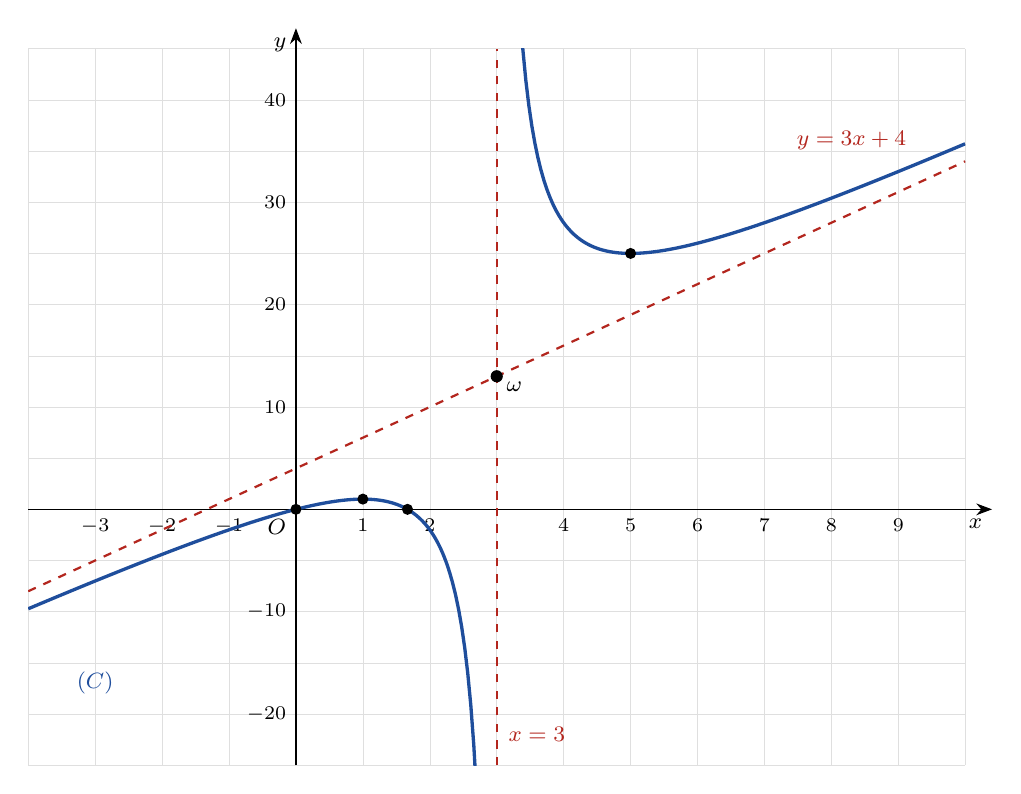
\begin{tikzpicture}[x=0.85cm,y=0.13cm,font=\footnotesize]
\draw[gray!25,very thin,xstep=1,ystep=5] (-4,-25) grid (10,45);
\draw[-{Stealth[length=2mm]}] (-4,0)--(10.4,0) node[below left]{$x$};
\draw[-{Stealth[length=2mm]}] (0,-25)--(0,47) node[below left]{$y$};
\foreach \t in {-3,-2,-1,1,2,4,5,6,7,8,9} \node[below,font=\scriptsize] at (\t,0){$\t$};
\foreach \t in {-20,-10,10,20,30,40} \node[left,font=\scriptsize] at (0,\t){$\t$};
\node[below left] at (0,0){$O$};
\begin{scope}\clip (-4,-25) rectangle (10,45);
\draw[cThm,dashed,thick](3,-25)--(3,45);
\draw[cThm,dashed,thick,domain=-4:10] plot(\x,{3*\x+4});
\draw[cDef,very thick,domain=-4:2.75,samples=150] plot(\x,{(3*\x*\x-5*\x)/(\x-3)});
\draw[cDef,very thick,domain=3.3:10,samples=150] plot(\x,{(3*\x*\x-5*\x)/(\x-3)});
\fill (0,0) circle(2pt) (5/3,0) circle(2pt) (1,1) circle(2pt) (5,25) circle(2pt) (3,13) circle(2.2pt);
\end{scope}
\node[right] at (3,12){$\omega$};
\node[cDef] at (-3,-17){$(C)$}; \node[cThm] at (8.3,36){$y=3x+4$}; \node[cThm] at (3.6,-22){$x=3$};
\end{tikzpicture}\end{LTR}\end{center}

\QQ{7} العدد $3$ ليس حلا (بالتعويض: $27-6\lambda-15+6\lambda=12\neq0$). من أجل $x\neq3$:
\[3x^{2}-(2\lambda+5)x+6\lambda=0\iff3x^{2}-5x=2\lambda x-6\lambda=2\lambda(x-3)\]\[\iff\frac{3x^{2}-5x}{x-3}=2\lambda\iff g(x)=2\lambda\]
الحلول فواصل نقط تقاطع $(C)$ مع المستقيم الأفقي $y=2\lambda$؛ ونستعين بـ $g(0)=g\left(\tfrac53\right)=0$:
\begin{itemize}
\item $2\lambda<0$، أي $\lambda<0$: حلان مختلفا الإشارة (في $]-\infty;0[$ وفي $\left]\tfrac53;3\right[$)؛
\item $\lambda=0$: حلان $0$ و $\tfrac53$؛
\item $0<2\lambda<1$، أي $0<\lambda<\tfrac12$: حلان موجبان (في $]0;1[$ وفي $\left]1;\tfrac53\right[$)؛
\item $\lambda=\tfrac12$: حل وحيد (مضاعف) $x=1$؛
\item $1<2\lambda<25$، أي $\tfrac12<\lambda<\tfrac{25}{2}$: لا توجد حلول؛
\item $\lambda=\tfrac{25}2$: حل وحيد (مضاعف) $x=5$؛
\item $\lambda>\tfrac{25}{2}$: حلان موجبان (في $]3;5[$ وفي $]5;+\infty[$).
\end{itemize}
(تحقق: $\lambda=-1$ يعطي $3x^{2}-3x-6=0$ أي $x=-1$ أو $x=2$.)

\textbf{الجزء الثالث:}
\begin{itemize}[label=$\clubsuit$]
\item $\varphi(x)$ معرّفة إذا وفقط إذا كان $|x|-3\neq0$ أي $x\neq3$ و $x\neq-3$: \bx{D_\varphi=\R-\{-3;3\}}.
\item $\varphi(0)=0$. من أجل $x>0$ ($x\neq3$): $\varphi(x)=\dfrac{3x^{2}-5x}{x-3}$، ومن أجل $x<0$ ($x\neq-3$): $\varphi(x)=\dfrac{3x^{2}+5x}{-x-3}$.
\[\lim_{x\to0^{+}}\frac{\varphi(x)-\varphi(0)}{x}=\lim_{x\to0^{+}}\frac{3x-5}{x-3}=\frac53\qquad\qquad\lim_{x\to0^{-}}\frac{\varphi(x)-\varphi(0)}{x}=\lim_{x\to0^{-}}\frac{3x+5}{-x-3}=-\frac53\]
النهايتان منتهيتان ومختلفتان، إذن \bxt{$\varphi$ غير قابلة للاشتقاق عند $0$} (لكنها قابلة للاشتقاق على يمين $0$ وعلى يساره). \textbf{بيانيا:} النقطة $A(0;0)$ نقطة زاوية، يقبل عندها المنحنى نصفي مماسين $y=\tfrac53x$ ($x\geqslant0$) و $y=-\tfrac53x$ ($x\leqslant0$).
\item $D_\varphi$ متناظرة بالنسبة إلى $0$، و $|-x|=|x|$ و $(-x)^{2}=x^{2}$، ومنه $\varphi(-x)=\dfrac{3x^{2}-5|x|}{|x|-3}=\varphi(x)$: \bxt{$\varphi$ دالة زوجية}، ومنحناها متناظر بالنسبة إلى محور التراتيب.
\item من أجل $x\geqslant0$ ، $|x|=x$ ومنه $\varphi(x)=\dfrac{3x^{2}-5x}{x-3}=g(x)$، أي \bx{\varphi(x)=g(x)} على \bx{I=[0;3[\,\cup\,]3;+\infty[}.

\textbf{الرسم:} نرسم الجزء من $(C)$ الموافق لـ $x\geqslant0$، ثم نكمله بنظيره بالنسبة إلى محور التراتيب (لأن $\varphi$ زوجية).
\end{itemize}
\begin{center}\begin{LTR}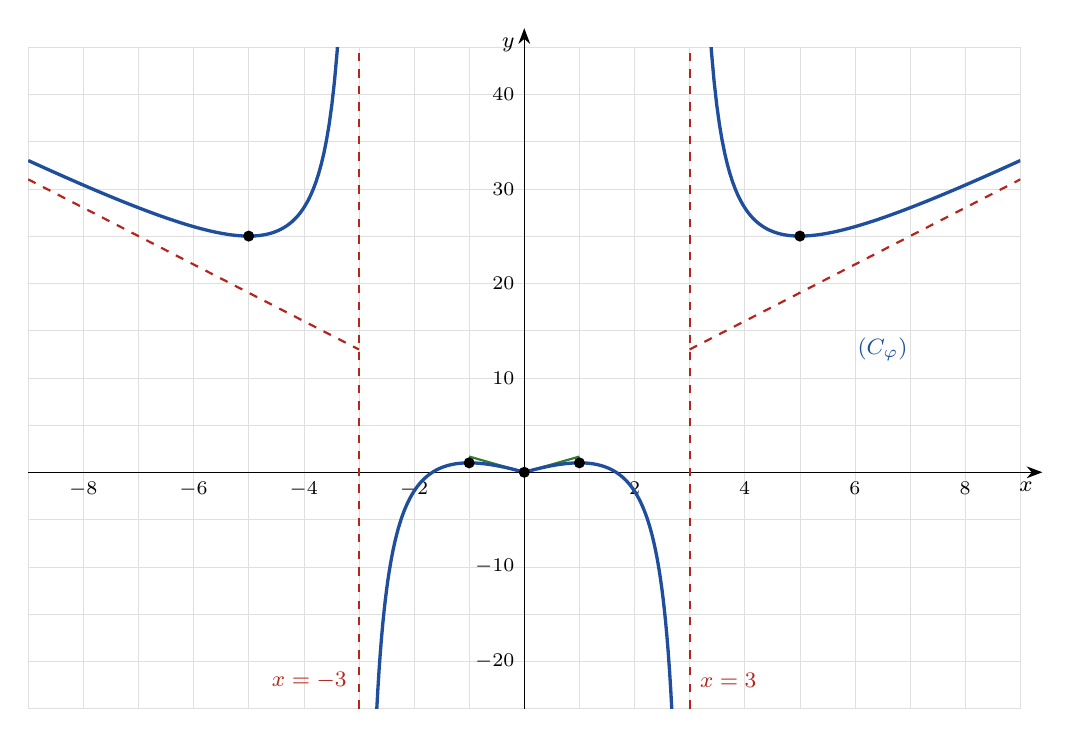
\begin{tikzpicture}[x=0.7cm,y=0.12cm,font=\footnotesize]
\draw[gray!25,very thin,xstep=1,ystep=5] (-9,-25) grid (9,45);
\draw[-{Stealth[length=2mm]}] (-9,0)--(9.4,0) node[below left]{$x$};
\draw[-{Stealth[length=2mm]}] (0,-25)--(0,47) node[below left]{$y$};
\foreach \t in {-8,-6,-4,-2,2,4,6,8} \node[below,font=\scriptsize] at (\t,0){$\t$};
\foreach \t in {-20,-10,10,20,30,40} \node[left,font=\scriptsize] at (0,\t){$\t$};
\begin{scope}\clip (-9,-25) rectangle (9,45);
\draw[cThm,dashed,thick](3,-25)--(3,45) (-3,-25)--(-3,45);
\draw[cThm,dashed,thick,domain=3:9] plot(\x,{3*\x+4});
\draw[cThm,dashed,thick,domain=-9:-3] plot(\x,{-3*\x+4});
\draw[cRem,thick,domain=-1:1] plot(\x,{5/3*abs(\x)});
\draw[cDef,very thick,domain=0:2.75,samples=120] plot(\x,{(3*\x*\x-5*\x)/(\x-3)});
\draw[cDef,very thick,domain=3.3:9,samples=120] plot(\x,{(3*\x*\x-5*\x)/(\x-3)});
\draw[cDef,very thick,domain=-2.75:0,samples=120] plot(\x,{(3*\x*\x+5*\x)/(-\x-3)});
\draw[cDef,very thick,domain=-9:-3.3,samples=120] plot(\x,{(3*\x*\x+5*\x)/(-\x-3)});
\fill (0,0) circle(2pt) (1,1) circle(2pt) (-1,1) circle(2pt) (5,25) circle(2pt) (-5,25) circle(2pt);
\end{scope}
\node[cDef] at (6.5,13){$(C_\varphi)$}; \node[cThm] at (3.7,-22){$x=3$}; \node[cThm] at (-3.9,-22){$x=-3$};
\end{tikzpicture}\end{LTR}\end{center}
\end{hal}

% ===================== تمرين 4 =====================
\begin{tamrin}{تمرين بمستوى البكالوريا: دالة مساعدة، حصر $f(\alpha)$ ومماسات موازية}
\textbf{I.} $g$ دالة معرّفة على $\R$ بـ: $g(x)=x^{3}+3x+8$.
\QQ{1} ادرس تغيّرات الدالة $g$ على $\R$ ثم شكّل جدول تغيّراتها.
\QQ{2} بيّن أن المعادلة $g(x)=0$ تقبل حلا وحيدا $\alpha$ في المجال $]-1{,}6;-1{,}5[$.
\QQ{3} حدّد حسب قيم $x$ إشارة $g(x)$.

\textbf{II.} $f$ دالة معرّفة بـ: $f(x)=\dfrac{x^{3}-4}{x^{2}+1}$، وليكن $(C_f)$ تمثيلها في معلم متعامد ومتجانس.
\QQ{1} عيّن $D_f$ مجموعة تعريف الدالة $f$.
\QQ{2} ادرس نهايات الدالة $f$ عند أطراف مجموعة تعريفها.
\QQ{3} بيّن أنه من أجل كل $x$ من $D_f$: \ $f'(x)=\dfrac{x\,g(x)}{(x^{2}+1)^{2}}$.
\QQ{4} ادرس اتجاه تغيّر الدالة $f$ ثم شكّل جدول تغيّراتها.
\QQ{5} برهن أن $f(\alpha)=\dfrac32\alpha$، ثم عيّن حصرا للعدد $f(\alpha)$.
\QQ{6} عيّن الأعداد الحقيقية $a$ ، $b$ و $c$ بحيث يكون $f(x)=ax+\dfrac{bx+c}{x^{2}+1}$ لكل $x$ من $\R$، ثم استنتج أن المنحنى $(C_f)$ له مستقيم مقارب مائل $(\Delta)$ يطلب تعيين معادلته.
\QQ{7} ادرس وضعية المنحنى $(C_f)$ بالنسبة إلى $(\Delta)$.
\QQ{8} عيّن نقاط تقاطع المنحنى $(C_f)$ مع حاملي المحورين.
\QQ{9} برهن أن المنحنى $(C_f)$ يقبل مماسين موازيين للمستقيم $(\Delta)$.
\QQ{10} احسب $f(-1)$ ، $f(1)$ ، $f(2)$ ثم ارسم $(\Delta)$ و $(C_f)$.

\textbf{III.} لتكن $h$ الدالة المعرّفة على $\R$ بـ: $h(x)=\left[f(x)\right]^{2}$.
\begin{itemize}[label=$\spadesuit$]
\item أعط عبارة $h'(x)$ بدلالة $f'(x)$ و $f(x)$ من أجل كل $x$ من $\R$.
\item ادرس إشارة $h'(x)$ من أجل كل $x$ من $\R$ ثم استنتج اتجاه تغيّر الدالة $h$ مشكّلا جدول تغيّراتها.
\end{itemize}
\end{tamrin}

\begin{hal}
\textbf{الجزء الأول:}

\QQ{1} $\lim\limits_{x\to-\infty}g(x)=\lim\limits_{x\to-\infty}x^{3}=\bx{-\infty}$ و $\lim\limits_{x\to+\infty}g(x)=\lim\limits_{x\to+\infty}x^{3}=\bx{+\infty}$.
$g'(x)=3x^{2}+3=3(x^{2}+1)>0$ من أجل كل $x$، إذن \bxt{$g$ متزايدة تماما على $\R$}.
\begin{TAB}
\tkzTabInit[lgt=2,espcl=4]{$x$/1,$g'(x)$/1,$g(x)$/2}{$-\infty$,$+\infty$}
\tkzTabLine{,+,}
\tkzTabVar{-/$-\infty$,+/$+\infty$}
\end{TAB}

\QQ{2} $g$ مستمرة ومتزايدة تماما على $[-1{,}6;-1{,}5]$، و:
\[g(-1{,}6)=-4{,}096-4{,}8+8=-0{,}896<0\qquad\qquad g(-1{,}5)=-3{,}375-4{,}5+8=0{,}125>0\]
حسب مبرهنة القيم المتوسطة (وبما أن $g$ رتيبة تماما على $\R$) فإن المعادلة $g(x)=0$ تقبل حلا وحيدا $\alpha$ و \bx{-1{,}6<\alpha<-1{,}5} ($\alpha\approx-1{,}513$).

\QQ{3} $g$ متزايدة تماما و $g(\alpha)=0$:
\begin{TAB}
\tkzTabInit[lgt=2,espcl=3]{$x$/1,$g(x)$/1}{$-\infty$,$\alpha$,$+\infty$}
\tkzTabLine{,-,z,+,}
\end{TAB}

\textbf{الجزء الثاني:}

\QQ{1} $x^{2}+1\geqslant1>0$ من أجل كل $x$، إذن \bx{D_f=\R}.

\QQ{2} $\lim\limits_{x\to\pm\infty}f(x)=\lim\limits_{x\to\pm\infty}\dfrac{x^{3}}{x^{2}}=\lim\limits_{x\to\pm\infty}x$، إذن \bx{\lim_{x\to-\infty}f(x)=-\infty} و \bx{\lim_{x\to+\infty}f(x)=+\infty}.

\QQ{3} $f=\dfrac uv$ مع $u=x^{3}-4$ ، $u'=3x^{2}$ ، $v=x^{2}+1$ ، $v'=2x$:
\begin{align*}f'(x)&=\frac{3x^{2}(x^{2}+1)-2x(x^{3}-4)}{(x^{2}+1)^{2}}=\frac{3x^{4}+3x^{2}-2x^{4}+8x}{(x^{2}+1)^{2}}=\frac{x^{4}+3x^{2}+8x}{(x^{2}+1)^{2}}\\&=\bx{\frac{x\left(x^{3}+3x+8\right)}{(x^{2}+1)^{2}}=\frac{x\,g(x)}{(x^{2}+1)^{2}}}\end{align*}

\QQ{4} إشارة $f'(x)$ هي إشارة $x\,g(x)$. $f(0)=-4$.
\begin{TAB}
\tkzTabInit[lgt=2,espcl=3]{$x$/1,$x$/0.8,$g(x)$/0.8,$f'(x)$/0.8,$f(x)$/2.2}{$-\infty$,$\alpha$,$0$,$+\infty$}
\tkzTabLine{,-,t,-,z,+,}
\tkzTabLine{,-,z,+,t,+,}
\tkzTabLine{,+,z,-,z,+,}
\tkzTabVar{-/$-\infty$,+/$f(\alpha)$,-/$-4$,+/$+\infty$}
\end{TAB}
\bxt{$f$ متزايدة تماما على $]-\infty;\alpha]$ وعلى $[0;+\infty[$، ومتناقصة تماما على $[\alpha;0]$}.

\QQ{5} من $g(\alpha)=0$: $\alpha^{3}=-3\alpha-8$. إذن:
\[f(\alpha)=\frac{\alpha^{3}-4}{\alpha^{2}+1}=\frac{-3\alpha-12}{\alpha^{2}+1}\]\[\frac32\alpha\left(\alpha^{2}+1\right)=\frac{3\alpha^{3}+3\alpha}{2}=\frac{3(-3\alpha-8)+3\alpha}{2}=-3\alpha-12\]
ومنه $\dfrac{-3\alpha-12}{\alpha^{2}+1}=\dfrac32\alpha$، أي \bx{f(\alpha)=\frac32\alpha}.

الحصر: $-1{,}6<\alpha<-1{,}5$ نضرب في $\dfrac32>0$: \bx{-2{,}4<f(\alpha)<-2{,}25} ($f(\alpha)\approx-2{,}27$).

\QQ{6} القسمة الإقليدية: $x^{3}-4=x(x^{2}+1)-x-4$، ومنه $f(x)=x+\dfrac{-x-4}{x^{2}+1}$. بالمطابقة: \bx{a=1,\ b=-1,\ c=-4}.

$f(x)-x=\dfrac{-x-4}{x^{2}+1}$ و $\lim\limits_{x\to\pm\infty}\dfrac{-x-4}{x^{2}+1}=\lim\limits_{x\to\pm\infty}\dfrac{-x}{x^{2}}=\lim\limits_{x\to\pm\infty}\dfrac{-1}{x}=0$، إذن \bx{(\Delta):\ y=x} مقارب مائل لـ $(C_f)$ بجوار $\pm\infty$.

\QQ{7} إشارة $f(x)-x=\dfrac{-(x+4)}{x^{2}+1}$ هي إشارة $-(x+4)$:
\begin{TAB}
\tkzTabInit[lgt=3,espcl=4]{$x$/0.8,$f(x)-x$/0.8,\ar{الوضع النسبي}/1}{$-\infty$,$-4$,$+\infty$}
\tkzTabLine{,+,z,-,}
\tkzTabLine{,\hbox{\ar{\footnotesize $(C_f)$ فوق $(\Delta)$}},z,\hbox{\ar{\footnotesize $(C_f)$ تحت $(\Delta)$}},}
\end{TAB}
و $(C_f)$ يقطع $(\Delta)$ في النقطة $(-4;-4)$.

\QQ{8} مع محور التراتيب: $f(0)=-4$، النقطة \bx{(0;-4)}.
مع محور الفواصل: $f(x)=0\iff x^{3}-4=0$. الدالة $x\mapsto x^{3}-4$ مستمرة ومتزايدة تماما على $\R$ ونهايتاها $-\infty$ و $+\infty$، فلهذه المعادلة حل وحيد نرمز له بـ $\gamma$ ($\gamma^{3}=4$، ومن $1{,}58^{3}<4<1{,}59^{3}$ نجد $\gamma\approx1{,}59$). النقطة \bx{(\gamma;0)}.

\QQ{9} مماس موازٍ لـ $(\Delta)$ يعني $f'(x)=1$:
\[\frac{x^{4}+3x^{2}+8x}{(x^{2}+1)^{2}}=1\iff x^{4}+3x^{2}+8x=x^{4}+2x^{2}+1\iff x^{2}+8x-1=0\]
المميّز $\Delta=64+4=68>0$، فلها حلان: $x_1=-4+\sqrt{17}$ ($\approx0{,}12$) و $x_2=-4-\sqrt{17}$ ($\approx-8{,}12$). إذن \bxt{$(C_f)$ يقبل مماسين موازيين لـ $(\Delta)$} عند النقطتين ذواتي الفاصلتين $x_1$ و $x_2$. معادلة كل منهما $y=x+\big(f(x_0)-x_0\big)=x-\dfrac{x_0+4}{x_0^{2}+1}$، وبالحساب ($x_1^{2}+1=34-8\sqrt{17}$ ، $x_2^{2}+1=34+8\sqrt{17}$):
\[(T_1):\ y=x-2-\frac{\sqrt{17}}{2}\qquad\qquad(T_2):\ y=x-2+\frac{\sqrt{17}}{2}\]

\QQ{10} $f(-1)=\dfrac{-5}{2}=\bx{-2{,}5}$ ، \ $f(1)=\dfrac{-3}{2}=\bx{-1{,}5}$ ، \ $f(2)=\dfrac{4}{5}=\bx{0{,}8}$.
\begin{GR}{-7}{5}{-8}{5}{0.68}
\Ticks{-6,-5,-4,-3,-2,-1,1,2,3,4}{-7,-6,-5,-4,-3,-2,-1,1,2,3,4}
\draw[cThm,dashed,thick,domain=-7:5] plot(\x,{\x});
\draw[cRem,thick,domain=-3:5] plot(\x,{\x-2-sqrt(17)/2});
\draw[cDef,very thick,domain=-7:5,samples=200] plot(\x,{(\x*\x*\x-4)/(\x*\x+1)});
\fill (-1.513,-2.27) circle(2pt) (0,-4) circle(2pt) (1.587,0) circle(2pt) (-4,-4) circle(2pt) (-1,-2.5) circle(1.5pt) (1,-1.5) circle(1.5pt) (2,0.8) circle(1.5pt) (0.123,-3.94) circle(1.5pt);
\draw[densely dotted](-1.513,0)--(-1.513,-2.27);
\node[above,font=\scriptsize] at (-1.513,0){$\alpha$}; \node[below right,font=\scriptsize] at (1.55,0){$\gamma$};
\node[cDef] at (3.5,1.2){$(C_f)$}; \node[cThm] at (-5.6,-4.6){$(\Delta)$}; \node[cRem] at (4.2,-1.2){$(T_1)$};
\end{GR}
(المماس $(T_2)$ يمس المنحنى عند $x_2\approx-8{,}12$ خارج النافذة.)

\textbf{الجزء الثالث:}
\begin{itemize}[label=$\spadesuit$]
\item $h=f^{2}$ و $f$ قابلة للاشتقاق على $\R$، إذن $h$ قابلة للاشتقاق و \bx{h'(x)=2f'(x)\,f(x)}.
\item إشارة $f(x)$: $f$ تنعدم عند $\gamma$ فقط، و $f(x)<0$ لما $x<\gamma$ ($x^{3}<4$) و $f(x)>0$ لما $x>\gamma$. مع العلم $\alpha<0<\gamma$ و $h(\alpha)=\dfrac94\alpha^{2}\approx5{,}15$ ، $h(0)=16$ ، $h\left(\gamma\right)=0$:
\end{itemize}
\begin{TAB}
\tkzTabInit[lgt=2,espcl=2.6]{$x$/1,$f'(x)$/0.8,$f(x)$/0.8,$h'(x)$/0.8,$h(x)$/2.2}{$-\infty$,$\alpha$,$0$,$\gamma$,$+\infty$}
\tkzTabLine{,+,z,-,z,+,t,+,}
\tkzTabLine{,-,t,-,t,-,z,+,}
\tkzTabLine{,-,z,+,z,-,z,+,}
\tkzTabVar{+/$+\infty$,-/$\frac94\alpha^{2}$,+/$16$,-/$0$,+/$+\infty$}
\end{TAB}
\bxt{$h$ متناقصة تماما على $]-\infty;\alpha]$ وعلى $\left[0;\gamma\right]$، ومتزايدة تماما على $[\alpha;0]$ وعلى $\left[\gamma;+\infty\right[$}.
\end{hal}

% ===================== تمرين 5 =====================
\begin{tamrin}{تمرين بمستوى البكالوريا: مقارب مائل، مناقشة $|f(x)|$ ونقطة زاوية}
\textbf{I.} لتكن $g$ الدالة المعرّفة على $\R$ بـ: $g(x)=x^{3}+ax^{2}+bx+c$، و $(C_g)$ تمثيلها البياني.
\begin{itemize}[label=$\spadesuit$]
\item عيّن الأعداد الحقيقية $a$ ، $b$ ، $c$ حيث: $(C_g)$ يشمل النقطتين $A(1;0)$ ، $B(0;-5)$ ويقبل مماسا عند النقطة ذات الفاصلة $x_0=-1$ معادلته $y=-2x-6$.
\end{itemize}
نفرض فيما يلي أن: $a=3$ ، $b=1$ ، $c=-5$.
\QQ{1} ادرس تغيّرات الدالة $g$ على $\R$ ثم شكّل جدول تغيّراتها.
\QQ{2} احسب $g(1)$ ثم استنتج حسب قيم $x$ إشارة $g(x)$.

\textbf{II.} $f$ الدالة المعرّفة على $\R-\{-1\}$ بـ: $f(x)=\dfrac{x^{3}+3x^{2}+5x+5}{(x+1)^{2}}$ ، $(C_f)$ تمثيلها البياني في المستوي المنسوب إلى معلم متعامد ومتجانس $(O;\vec i,\vec j)$.
\QQ{1} احسب نهايات الدالة $f$ عند الأطراف المفتوحة لمجموعة التعريف.
\QQ{2} جد الأعداد الحقيقية $\alpha$ ، $\beta$ ، $\gamma$ ، $\lambda$ حتى يكون من أجل كل عدد حقيقي $x$ من $D_f$: \[f(x)=\alpha x+\beta+\frac{\gamma x+\lambda}{(x+1)^{2}}\]
\QQ{3} استنتج وجود مستقيم مقارب مائل $(\Delta)$ للمنحنى $(C_f)$ يطلب تعيين معادلته، ثم ادرس الوضع النسبي بينهما.
\QQ{4} بيّن أنه من أجل كل $x\neq-1$: \ $f'(x)=\dfrac{g(x)}{(x+1)^{3}}$.
\QQ{5} عيّن دون حساب: $\displaystyle\lim_{x\to1}\left(\frac{f(x)-f(1)}{x-1}\right)$ مفسّرا النتيجة بيانيا.
\QQ{6} ادرس اتجاه تغيّر الدالة $f$ وشكّل جدول تغيّراتها.
\QQ{7} بيّن أن المنحنى $(C_f)$ يقبل مماسا $(T)$ موازيا للمستقيم $(\Delta)$ يطلب كتابة معادلته. برّر أن المعادلة $f(x)=0$ تقبل حلا وحيدا $\theta$ في المجال $]-2;-1[$.
\QQ{8} ادرس نقاط تقاطع المنحنى $(C_f)$ مع حاملي المحورين ثم أنشئ بدقة $(\Delta)$ ، $(T)$ و $(C_f)$.
\QQ{9} ناقش بيانيا وحسب قيم الوسيط الحقيقي $\sigma$ عدد وإشارة حلول المعادلة: \ $|f(x)|=-\dfrac12\sigma+1$.

\textbf{III.} لتكن $h$ الدالة المعرّفة على $\R$ بـ: $h(x)=\dfrac{|x|^{3}+3x^{2}+5|x|+5}{\left(|x|+1\right)^{2}}$ ، $(C_h)$ تمثيلها البياني.
\begin{itemize}[label=$\star$]
\item بيّن أن $h$ دالة زوجية.
\item ادرس استمرارية الدالة $h$ عند النقطة ذات الفاصلة $0$.
\item بيّن أن: $\displaystyle\lim_{\substack{x\to0\\x<0}}\frac{h(x)-h(0)}{x}\neq\lim_{\substack{x\to0\\x>0}}\frac{h(x)-h(0)}{x}$ ثم فسّر النتيجة بيانيا.
\item اشرح كيفية رسم المنحنى $(C_h)$ انطلاقا من $(C_f)$ بعد نزع القيمة المطلقة لـ $h$.
\end{itemize}
\end{tamrin}

\begin{hal}
\textbf{الجزء الأول:} $g'(x)=3x^{2}+2ax+b$.
\begin{itemize}[label=$\spadesuit$]
\item $B(0;-5)\in(C_g)\iff g(0)=-5\iff c=-5$.
\item $A(1;0)\in(C_g)\iff1+a+b+c=0\iff a+b=4$.
\item المماس عند $-1$ هو $y=-2x-6$: معامل توجيهه $g'(-1)=-2$، ونقطة التماس عليه: $g(-1)=-2(-1)-6=-4$.
\[g'(-1)=3-2a+b=-2\iff-2a+b=-5\]\[g(-1)=-1+a-b+c=-4\iff a-b=2\]
\end{itemize}
من $a+b=4$ و $a-b=2$: $a=3$ و $b=1$، والتحقق: $-2(3)+1=-5$ \ok. إذن \bx{a=3,\ b=1,\ c=-5} و $g(x)=x^{3}+3x^{2}+x-5$.

\QQ{1} $\lim\limits_{x\to-\infty}g(x)=\lim\limits_{x\to-\infty}x^{3}=-\infty$ و $\lim\limits_{x\to+\infty}g(x)=+\infty$.
$g'(x)=3x^{2}+6x+1$، مميّزه $\Delta=36-12=24$، وجذراه $x_1=\dfrac{-6-2\sqrt6}{6}=-1-\dfrac{\sqrt6}{3}\approx-1{,}82$ و $x_2=-1+\dfrac{\sqrt6}{3}\approx-0{,}18$.
بكتابة $g(x)=(x+1)^{3}-2(x+1)-4$ نجد: $g(x_1)=-4+\dfrac{4\sqrt6}{9}\approx-2{,}91$ و $g(x_2)=-4-\dfrac{4\sqrt6}{9}\approx-5{,}09$.
\begin{TAB}
\tkzTabInit[lgt=2,espcl=3]{$x$/1,$g'(x)$/1,$g(x)$/2.2}{$-\infty$,$x_1$,$x_2$,$+\infty$}
\tkzTabLine{,+,z,-,z,+,}
\tkzTabVar{-/$-\infty$,+/$-4+\frac{4\sqrt6}{9}$,-/$-4-\frac{4\sqrt6}{9}$,+/$+\infty$}
\end{TAB}

\QQ{2} $g(1)=1+3+1-5=\bx{0}$.
على $]-\infty;x_2]$: القيمة الحدية العظمى $g(x_1)<0$، فـ $g(x)<0$. على $[x_2;+\infty[$: $g$ متزايدة تماما وتنعدم عند $1$. إذن:
\begin{TAB}
\tkzTabInit[lgt=2,espcl=3]{$x$/1,$g(x)$/1}{$-\infty$,$1$,$+\infty$}
\tkzTabLine{,-,z,+,}
\end{TAB}
(تأكيد: $g(x)=(x-1)(x^{2}+4x+5)$ و $x^{2}+4x+5=(x+2)^{2}+1>0$.)

\textbf{الجزء الثاني:}

\QQ{1} $\lim\limits_{x\to\pm\infty}f(x)=\lim\limits_{x\to\pm\infty}\dfrac{x^{3}}{x^{2}}=\lim\limits_{x\to\pm\infty}x$: \bx{\lim_{x\to-\infty}f(x)=-\infty} و \bx{\lim_{x\to+\infty}f(x)=+\infty}.

عند $-1$: البسط يؤول إلى $-1+3-5+5=2>0$ والمقام $(x+1)^{2}\to0^{+}$ من الجهتين: \bx{\lim_{x\to-1^{-}}f(x)=\lim_{x\to-1^{+}}f(x)=+\infty}.

\QQ{2} القسمة الإقليدية لـ $x^{3}+3x^{2}+5x+5$ على $(x+1)^{2}=x^{2}+2x+1$:
\[x^{3}+3x^{2}+5x+5=(x+1)(x^{2}+2x+1)+2x+4\]
(لأن $(x+1)(x^{2}+2x+1)=x^{3}+3x^{2}+3x+1$.) ومنه \bx{f(x)=x+1+\frac{2x+4}{(x+1)^{2}}}، أي \bx{\alpha=1,\ \beta=1,\ \gamma=2,\ \lambda=4}.

\QQ{3} $f(x)-(x+1)=\dfrac{2x+4}{(x+1)^{2}}$ و $\lim\limits_{x\to\pm\infty}\dfrac{2x+4}{x^{2}+2x+1}=\lim\limits_{x\to\pm\infty}\dfrac{2}{x}=0$: \bx{(\Delta):\ y=x+1} مقارب مائل بجوار $\pm\infty$.

إشارة الفرق هي إشارة $2x+4$ (المقام موجب):
\begin{TAB}
\tkzTabInit[lgt=3,espcl=3.5]{$x$/0.8,$f(x)-y$/0.8,\ar{الوضع النسبي}/1}{$-\infty$,$-2$,$-1$,$+\infty$}
\tkzTabLine{,-,z,+,d,+,}
\tkzTabLine{,\hbox{\ar{\footnotesize $(C_f)$ تحت $(\Delta)$}},z,\hbox{\ar{\footnotesize فوق $(\Delta)$}},d,\hbox{\ar{\footnotesize $(C_f)$ فوق $(\Delta)$}},}
\end{TAB}
و $(C_f)$ يقطع $(\Delta)$ في النقطة $(-2;-1)$.

\QQ{4} من $f(x)=x+1+\dfrac{2x+4}{(x+1)^{2}}$:
\[\left(\frac{2x+4}{(x+1)^{2}}\right)'=\frac{2(x+1)^{2}-(2x+4)\cdot2(x+1)}{(x+1)^{4}}=\frac{2(x+1)-2(2x+4)}{(x+1)^{3}}=\frac{-2x-6}{(x+1)^{3}}\]
\[f'(x)=1+\frac{-2x-6}{(x+1)^{3}}=\frac{x^{3}+3x^{2}+3x+1-2x-6}{(x+1)^{3}}=\bx{\frac{x^{3}+3x^{2}+x-5}{(x+1)^{3}}=\frac{g(x)}{(x+1)^{3}}}\]

\QQ{5} $f$ قابلة للاشتقاق عند $1$، والنهاية المطلوبة هي العدد المشتق $f'(1)=\dfrac{g(1)}{2^{3}}=0$: \bx{\lim_{x\to1}\frac{f(x)-f(1)}{x-1}=0}.
\textbf{بيانيا:} $(C_f)$ يقبل عند النقطة $\left(1;\tfrac72\right)$ مماسا موازيا لمحور الفواصل (لأن $f(1)=\tfrac{14}{4}=\tfrac72$).

\QQ{6} إشارة $f'(x)$ هي إشارة $\dfrac{g(x)}{(x+1)^{3}}$، وإشارة $(x+1)^{3}$ هي إشارة $x+1$:
\begin{TAB}
\tkzTabInit[lgt=2,espcl=3]{$x$/1,$g(x)$/0.8,$(x+1)^{3}$/0.8,$f'(x)$/0.8,$f(x)$/2.2}{$-\infty$,$-1$,$1$,$+\infty$}
\tkzTabLine{,-,t,-,z,+,}
\tkzTabLine{,-,z,+,t,+,}
\tkzTabLine{,+,d,-,z,+,}
\tkzTabVar{-/$-\infty$,+D+/$+\infty$/$+\infty$,-/$\frac72$,+/$+\infty$}
\end{TAB}
\bxt{$f$ متزايدة تماما على $]-\infty;-1[$ وعلى $[1;+\infty[$، ومتناقصة تماما على $]-1;1]$}.

\QQ{7} \textbf{المماس الموازي:} $f'(x)=1\iff g(x)=(x+1)^{3}$. وبما أن $g(x)=(x+1)^{3}-2(x+1)-4$:
\[(x+1)^{3}-2(x+1)-4=(x+1)^{3}\iff-2x-6=0\iff x=-3\]
$f(-3)=\dfrac{-27+27-15+5}{4}=-\dfrac52$، إذن $(T):\ y=1\cdot(x+3)-\dfrac52$ أي \bx{(T):\ y=x+\tfrac12}.

\textbf{الحل $\theta$:} $f$ مستمرة ومتزايدة تماما على $]-\infty;-1[$، و $f(-2)=\dfrac{-8+12-10+5}{1}=-1<0$ و $\lim\limits_{x\to-1^{-}}f(x)=+\infty$. فحسب مبرهنة القيم المتوسطة (صورة المجال $[-2;-1[$ هي $[-1;+\infty[$ التي تشمل $0$) يوجد عدد وحيد $\theta\in]-2;-1[$ حيث $f(\theta)=0$. وعلى $]-1;+\infty[$ لدينا $f(x)\geqslant\tfrac72>0$، فـ $\theta$ هو الحل الوحيد في $D_f$ ($\theta\approx-1{,}77$).

\QQ{8} مع محور التراتيب: $f(0)=5$، النقطة \bx{(0;5)}. مع محور الفواصل: النقطة الوحيدة \bx{(\theta;0)}.
\par\noindent\begin{minipage}{\linewidth}
\begin{GR}{-6}{5}{-6}{10}{0.68}
\Ticks{-5,-4,-3,-2,-1,1,2,3,4}{-5,-4,-3,-2,-1,1,2,3,4,5,6,7,8,9}
\draw[cThm,dashed,thick](-1,-6)--(-1,10);
\draw[cThm,dashed,thick,domain=-6:5] plot(\x,{\x+1});
\draw[cEx,thick,domain=-6:5] plot(\x,{\x+0.5});
\draw[cRem,thick,densely dashed,domain=-6:-1.771,samples=100] plot(\x,{-(\x*\x*\x+3*\x*\x+5*\x+5)/((\x+1)*(\x+1))});
\draw[cDef,very thick,domain=-6:-1.3,samples=200] plot(\x,{(\x*\x*\x+3*\x*\x+5*\x+5)/((\x+1)*(\x+1))});
\draw[cDef,very thick,domain=-0.55:5,samples=200] plot(\x,{(\x*\x*\x+3*\x*\x+5*\x+5)/((\x+1)*(\x+1))});
\draw[cRem,thick](0.6,3.5)--(1.4,3.5);
\fill (-1.771,0) circle(2pt) (0,5) circle(2pt) (1,3.5) circle(2pt) (-2,-1) circle(2pt) (-3,-2.5) circle(2pt);
\node[below left] at (-1.77,0){$\theta$};
\node[cDef] at (4,8.2){$(C_f)$}; \node[cThm] at (-5.2,-3.2){$(\Delta)$}; \node[cEx] at (-4.6,-4.9){$(T)$};
\node[cRem] at (-4.3,4.6){$y=-f(x)$}; \node[cThm] at (-1.6,-5.5){$x=-1$};
\end{GR}
\end{minipage}
(الجزء المتقطع الأخضر هو نظير جزء $(C_f)$ الواقع تحت محور الفواصل، أي لـ $x<\theta$، ويُستعمل في السؤال 9.)

\QQ{9} \textbf{منحنى $|f|$:} $|f(x)|=f(x)$ لما $f(x)\geqslant0$ أي $x\geqslant\theta$، و $|f(x)|=-f(x)$ لما $x<\theta$. فمنحنى $|f|$ ينطبق على $(C_f)$ لما $x\geqslant\theta$، ويكون نظير $(C_f)$ بالنسبة إلى محور الفواصل لما $x<\theta$.
فهو: متناقص من $+\infty$ إلى $0$ على $]-\infty;\theta]$، متزايد من $0$ إلى $+\infty$ على $[\theta;-1[$، متناقص من $+\infty$ إلى $\tfrac72$ على $]-1;1]$ (مارا بـ $(0;5)$)، ومتزايد من $\tfrac72$ إلى $+\infty$ على $[1;+\infty[$.

نضع $k=-\dfrac12\sigma+1$ (المستقيم الأفقي $y=k$):
\begin{itemize}
\item $k<0$ أي $\sigma>2$: لا توجد حلول؛
\item $k=0$ أي $\sigma=2$: حل وحيد $x=\theta$ (سالب)؛
\item $0<k<\tfrac72$ أي $-5<\sigma<2$: حلان سالبان (أحدهما أصغر من $\theta$ والآخر في $]\theta;-1[$)؛
\item $k=\tfrac72$ أي $\sigma=-5$: ثلاثة حلول: حلان سالبان و $x=1$؛
\item $\tfrac72<k<5$ أي $-8<\sigma<-5$: أربعة حلول: حلان سالبان وحلان موجبان (في $]0;1[$ وفي $]1;+\infty[$)؛
\item $k=5$ أي $\sigma=-8$: أربعة حلول: حلان سالبان، حل معدوم $x=0$ وحل موجب؛
\item $k>5$ أي $\sigma<-8$: أربعة حلول: ثلاثة سالبة (أحدها في $]-1;0[$) وحل موجب.
\end{itemize}

\textbf{الجزء الثالث:}
\begin{itemize}[label=$\star$]
\item $D_h=\R$ متناظرة، و $|x|^{3}=\left(|x|\right)^{3}$ ، $x^{2}=|x|^{2}$، ومنه $h(x)=\dfrac{|x|^{3}+3|x|^{2}+5|x|+5}{(|x|+1)^{2}}=f(|x|)$. وبما أن $|-x|=|x|$ فإن $h(-x)=h(x)$: \bxt{$h$ دالة زوجية}.
\item $x\mapsto|x|$ مستمرة على $\R$ و $f$ مستمرة على $[0;+\infty[$، فـ $h=f\circ|\cdot|$ مستمرة عند $0$، و $\lim\limits_{x\to0}h(x)=f(0)=5=h(0)$.
\item من أجل $x>0$: $\dfrac{h(x)-h(0)}{x}=\dfrac{f(x)-f(0)}{x-0}\xrightarrow[x\to0^{+}]{}f'(0)=\dfrac{g(0)}{1}=-5$.

من أجل $x<0$: $h(x)=f(-x)$، ومنه $\dfrac{h(x)-h(0)}{x}=-\dfrac{f(-x)-f(0)}{-x-0}\xrightarrow[x\to0^{-}]{}-f'(0)=5$.

إذن \bx{\lim_{x\to0^{-}}\frac{h(x)-h(0)}{x}=5\neq-5=\lim_{x\to0^{+}}\frac{h(x)-h(0)}{x}}: \bxt{$h$ غير قابلة للاشتقاق عند $0$}.
\textbf{بيانيا:} النقطة $(0;5)$ نقطة زاوية لـ $(C_h)$، وله عندها نصفا مماسين: $y=-5x+5$ ($x\geqslant0$) و $y=5x+5$ ($x\leqslant0$).
\item \textbf{الرسم:} $h(x)=f(x)$ من أجل $x\geqslant0$، و $h(x)=f(-x)$ من أجل $x\leqslant0$. نرسم جزء $(C_f)$ الموافق لـ $x\geqslant0$، ثم نظيره بالنسبة إلى محور التراتيب.
\end{itemize}
\begin{GR}{-5}{5}{-1}{8}{0.6}
\Ticks{-4,-3,-2,-1,1,2,3,4}{1,2,3,4,5,6,7}
\draw[cRem,thick,domain=-0.5:0.5] plot(\x,{5-5*abs(\x)});
\draw[cDef,very thick,domain=0:5,samples=150] plot(\x,{(\x*\x*\x+3*\x*\x+5*\x+5)/((\x+1)*(\x+1))});
\draw[cDef,very thick,domain=-5:0,samples=150] plot(\x,{(-\x*\x*\x+3*\x*\x-5*\x+5)/((-\x+1)*(-\x+1))});
\fill (0,5) circle(2pt) (1,3.5) circle(2pt) (-1,3.5) circle(2pt);
\node[cDef] at (3.6,6.6){$(C_h)$};
\end{GR}
\end{hal}

% ===================== تمرين 6 =====================
\begin{tamrin}{تمرين بمستوى البكالوريا: دالة صماء، مقارب مائل ومناقشة $g(x)=m^{2}$}
نعتبر $f$ الدالة المعرّفة على المجال $]-1;+\infty[$ بـ: $f(x)=x-\dfrac{2}{\sqrt{x+1}}$، و $(C)$ تمثيلها البياني.
\QQ{1} ادرس تغيّرات الدالة $f$ على المجال $]-1;+\infty[$.
\QQ{2} بيّن أن $(C)$ يقبل مستقيمين مقاربين أحدهما المستقيم $(\Delta)$ ذو المعادلة $y=x$، ثم ادرس الوضع النسبي بين $(C)$ و $(\Delta)$.
\QQ{3} بيّن أن المنحنى $(C)$ يقطع حامل محور الفواصل في نقطة وحيدة فاصلتها $x_0$ حيث: $1{,}3<x_0<1{,}4$.
\QQ{4} عيّن معادلة المماس $(T)$ للمنحنى $(C)$ عند نقطة تقاطعه مع حامل محور التراتيب.
\QQ{5} ارسم $(T)$ ، $(\Delta)$ و $(C)$.
\QQ{6} $g$ الدالة المعرّفة على $]-1;+\infty[$ بـ: $g(x)=|f(x)|$، و $(C_g)$ منحناها البياني.
\begin{itemize}[label=$\star$]
\item بيّن كيفية إنشاء $(C_g)$ انطلاقا من $(C)$ ثم أنشئه في المعلم السابق.
\item ناقش بيانيا حسب قيم الوسيط الحقيقي $m$ عدد وإشارة حلول المعادلة: $g(x)=m^{2}$.
\end{itemize}
\end{tamrin}

\begin{hal}
\QQ{1} \textbf{النهايات:} لما $x\to-1^{+}$: $\sqrt{x+1}\to0^{+}$ ومنه $\dfrac{2}{\sqrt{x+1}}\to+\infty$، إذن \bx{\lim_{x\to-1^{+}}f(x)=-1-\infty=-\infty}.
لما $x\to+\infty$: $\dfrac{2}{\sqrt{x+1}}\to0$، إذن \bx{\lim_{x\to+\infty}f(x)=+\infty}.

\textbf{المشتقة:} $\left(\dfrac{1}{\sqrt u}\right)'=-\dfrac{u'}{2u\sqrt u}$، ومنه:
\[f'(x)=1-2\times\left(-\frac{1}{2(x+1)\sqrt{x+1}}\right)=1+\frac{1}{(x+1)\sqrt{x+1}}>0\]
\begin{TAB}
\tkzTabInit[lgt=2,espcl=4]{$x$/1,$f'(x)$/1,$f(x)$/2}{$-1$,$+\infty$}
\tkzTabLine{d,+,}
\tkzTabVar{D-/$-\infty$,+/$+\infty$}
\end{TAB}
\bxt{$f$ متزايدة تماما على $]-1;+\infty[$}.

\QQ{2} \begin{itemize}
\item $\lim\limits_{x\to-1^{+}}f(x)=-\infty$: المستقيم \bx{x=-1} مقارب عمودي.
\item $f(x)-x=-\dfrac{2}{\sqrt{x+1}}\xrightarrow[x\to+\infty]{}0$: المستقيم \bx{(\Delta):\ y=x} مقارب مائل بجوار $+\infty$.
\end{itemize}
\textbf{الوضع النسبي:} $f(x)-x=-\dfrac{2}{\sqrt{x+1}}<0$ من أجل كل $x>-1$: \bxt{$(C)$ يقع تحت $(\Delta)$ على $]-1;+\infty[$}.

\QQ{3} $f$ مستمرة ومتزايدة تماما على $[1{,}3;1{,}4]$، و:
\[f(1{,}3)=1{,}3-\frac{2}{\sqrt{2{,}3}}\approx1{,}3-1{,}319=-0{,}019<0\]\[f(1{,}4)=1{,}4-\frac{2}{\sqrt{2{,}4}}\approx1{,}4-1{,}291=0{,}109>0\]
حسب مبرهنة القيم المتوسطة، ولأن $f$ تقابل من $]-1;+\infty[$ نحو $\R$، المعادلة $f(x)=0$ تقبل حلا وحيدا $x_0$ و \bx{1{,}3<x_0<1{,}4} ($x_0\approx1{,}315$).

\QQ{4} $f(0)=0-\dfrac{2}{1}=-2$ و $f'(0)=1+1=2$: \ $(T):\ y=2(x-0)-2$ أي \bx{(T):\ y=2x-2}.

\QQ{5} نقط مساعدة: $f(3)=3-1=2$ ، $f(8)=8-\tfrac23\approx7{,}33$ ، $f(-0{,}75)=-0{,}75-4=-4{,}75$.
\begin{GR}{-1.5}{6}{-6}{6}{0.72}
\Ticks{-1,1,2,3,4,5}{-5,-4,-3,-2,-1,1,2,3,4,5}
\draw[cThm,dashed,thick](-1,-6)--(-1,6);
\draw[cThm,dashed,thick,domain=-1.5:6] plot(\x,{\x});
\draw[cEx,thick,domain=-1.5:3.5] plot(\x,{2*\x-2});
\draw[cRem,thick,densely dashed,domain=-0.86:1.315,samples=150] plot(\x,{-(\x-2/sqrt(\x+1))});
\draw[cDef,very thick,domain=-0.86:6,samples=200] plot(\x,{\x-2/sqrt(\x+1)});
\fill (0,-2) circle(2pt) (1.315,0) circle(2pt) (3,2) circle(1.6pt) (0,2) circle(2pt);
\node[below right] at (1.3,0){$x_0$};
\node[cDef] at (5,2.9){$(C)$}; \node[cThm] at (5.2,5.6){$(\Delta)$}; \node[cEx] at (3.4,3.6){$(T)$}; \node[cRem] at (0.75,4.6){$(C_g)$};
\end{GR}

\QQ{6}
\begin{itemize}[label=$\star$]
\item $g(x)=f(x)$ لما $f(x)\geqslant0$ أي $x\geqslant x_0$، و $g(x)=-f(x)$ لما $-1<x<x_0$. إذن \bxt{$(C_g)$ ينطبق على $(C)$ على $[x_0;+\infty[$، وهو نظير $(C)$ بالنسبة إلى محور الفواصل على $]-1;x_0]$} (الجزء المتقطع الأخضر في الشكل مع الجزء من $(C)$ الواقع فوق محور الفواصل).
\item $g$ متناقصة تماما من $+\infty$ إلى $0$ على $]-1;x_0]$ ومتزايدة تماما من $0$ إلى $+\infty$ على $[x_0;+\infty[$، و $g(0)=|-2|=2$. الحلول هي فواصل نقط تقاطع $(C_g)$ مع المستقيم الأفقي $y=m^{2}$ (مع $m^{2}\geqslant0$):
\begin{itemize}
\item $m=0$: حل وحيد $x_0$ (موجب)؛
\item $0<m^{2}<2$ أي $m\in\left]-\sqrt2;0\right[\,\cup\,\left]0;\sqrt2\right[$: حلان موجبان (في $]0;x_0[$ وفي $]x_0;+\infty[$)؛
\item $m^{2}=2$ أي $m=-\sqrt2$ أو $m=\sqrt2$: حلان، أحدهما معدوم $x=0$ والآخر موجب؛
\item $m^{2}>2$ أي $m<-\sqrt2$ أو $m>\sqrt2$: حلان مختلفا الإشارة (في $]-1;0[$ وفي $]x_0;+\infty[$).
\end{itemize}
\end{itemize}
\end{hal}

% ===================== تمرين 7 =====================
\begin{tamrin}{تمرين بمستوى البكالوريا: دالة ناطقة، دالة زوجية وعائلة منحنيات -- شعبة رياضيات}
\textbf{I.} نعتبر $f$ الدالة المعرّفة بـ: $f(x)=\dfrac{x^{2}+ax+b}{x^{2}+x-6}$.
\QQ{1} حدّد مجموعة تعريف الدالة $f$.
\QQ{2} جد العددين الحقيقيين $a$ و $b$ بحيث المنحنى $(C_f)$ يشمل النقطة $A(0;1)$ ويقبل مماسا معامل توجيهه $-\dfrac74$ عند النقطة ذات الفاصلة $x_0=1$.

\textbf{II.} لتكن الدالة $g$ المعرّفة على $\R-\{-3;2\}$ بـ: $g(x)=\dfrac{x^{2}+5x-6}{x^{2}+x-6}$.
\QQ{1} احسب نهايات الدالة $g$ عند حدود مجالات مجموعة التعريف.
\QQ{2} ادرس اتجاه تغيّر الدالة $g$ على مجموعة تعريفها.
\QQ{3} اكتب معادلة المماس $(T)$ عند النقطة ذات الفاصلة $x_0=1$.
\QQ{4} جد معادلات المستقيمات المقاربة للمنحنى $(C_g)$.
\QQ{5} ادرس وضعية المنحنى $(C_g)$ بالنسبة إلى المستقيم $(\Delta)$ ذي المعادلة: $y=1$.
\QQ{6} ارسم المنحنى $(C_g)$ والمستقيمات المقاربة.
\QQ{7} ناقش بيانيا حسب قيم الوسيط الحقيقي $m$ عدد وإشارة حلول المعادلة: \ $(m+1)x^{2}+(m+5)x-6m-6=0$.

\textbf{III.} لتكن الدالة $h$ المعرّفة بـ: $h(x)=\dfrac{x^{2}+5|x|-6}{x^{2}+|x|-6}$.
\QQ{1} جد مجموعة تعريف الدالة $h$.
\QQ{2} برهن أن الدالة $h$ زوجية وفسّر النتيجة بيانيا.
\QQ{3} اكتب $h(x)$ دون رمز القيمة المطلقة.
\QQ{4} عبّر عن $h$ بدلالة $g$ على مجال يطلب تعيينه.
\QQ{5} بيّن كيف يمكن إنشاء $(C_h)$ انطلاقا من $(C_g)$.

\textbf{IV.} لتكن الدالة $k_m$ المعرّفة بـ: $k_m(x)=\dfrac{x^{2}+5mx-6}{x^{2}+mx-6}$ ، حيث $m$ وسيط حقيقي.
\begin{itemize}[label=$\star$]
\item بيّن أن جميع المنحنيات $(C_{k_m})$ تشمل ثلاث نقاط ثابتة يطلب تعيين إحداثياتها.
\item ما هو المنحنى $(C_{k_m})$ الذي يشمل النقطة $B(-2;3)$؟
\end{itemize}
\end{tamrin}

\begin{hal}
\textbf{الجزء الأول:}

\QQ{1} $x^{2}+x-6=(x+3)(x-2)$ ينعدم عند $-3$ و $2$: \bx{D_f=\R-\{-3;2\}}.

\QQ{2} $A(0;1)\in(C_f)\iff f(0)=1\iff\dfrac{b}{-6}=1\iff\bx{b=-6}$.

$f'(x)=\dfrac{(2x+a)(x^{2}+x-6)-(x^{2}+ax+b)(2x+1)}{(x^{2}+x-6)^{2}}$، ومع $b=-6$:
\[f'(1)=\frac{(2+a)(-4)-(a-5)(3)}{(-4)^{2}}=\frac{-8-4a-3a+15}{16}=\frac{7-7a}{16}\]
$f'(1)=-\dfrac74\iff7-7a=-28\iff\bx{a=5}$. إذن $f(x)=\dfrac{x^{2}+5x-6}{x^{2}+x-6}$، وهي الدالة $g$ في الجزء الثاني.

\textbf{الجزء الثاني:} نلاحظ أن $x^{2}+5x-6=(x^{2}+x-6)+4x$، ومنه \bx{g(x)=1+\frac{4x}{x^{2}+x-6}=1+\frac{4x}{(x+3)(x-2)}}.

\QQ{1} \begin{itemize}
\item $\lim\limits_{x\to\pm\infty}g(x)=\lim\limits_{x\to\pm\infty}\dfrac{x^{2}}{x^{2}}=\bx{1}$.
\item عند $-3$: البسط $9-15-6=-12<0$، و $(x+3)(x-2)\to0^{+}$ لما $x\to-3^{-}$ (جداء عددين سالبين) و $\to0^{-}$ لما $x\to-3^{+}$:
\bx{\lim_{x\to-3^{-}}g(x)=-\infty} و \bx{\lim_{x\to-3^{+}}g(x)=+\infty}.
\item عند $2$: البسط $4+10-6=8>0$، و $(x+3)(x-2)\to0^{-}$ لما $x\to2^{-}$ و $\to0^{+}$ لما $x\to2^{+}$:
\bx{\lim_{x\to2^{-}}g(x)=-\infty} و \bx{\lim_{x\to2^{+}}g(x)=+\infty}.
\end{itemize}

\QQ{2} \[g'(x)=4\times\frac{(x^{2}+x-6)-x(2x+1)}{(x^{2}+x-6)^{2}}=\frac{4\left(-x^{2}-6\right)}{(x^{2}+x-6)^{2}}=\frac{-4\left(x^{2}+6\right)}{(x^{2}+x-6)^{2}}<0\]
\begin{TAB}
\tkzTabInit[lgt=2,espcl=3.2]{$x$/1,$g'(x)$/1,$g(x)$/2.2}{$-\infty$,$-3$,$2$,$+\infty$}
\tkzTabLine{,-,d,-,d,-,}
\tkzTabVar{+/$1$,-D+/$-\infty$/$+\infty$,-D+/$-\infty$/$+\infty$,-/$1$}
\end{TAB}
\bxt{$g$ متناقصة تماما على كل من $]-\infty;-3[$ ، $]-3;2[$ و $]2;+\infty[$}.

\QQ{3} $g(1)=\dfrac{0}{-4}=0$ و $g'(1)=\dfrac{-4\times7}{16}=-\dfrac74$: \ $(T):\ y=-\dfrac74(x-1)+0$ أي \bx{(T):\ y=-\tfrac74x+\tfrac74}.

\QQ{4} \bx{y=1} مقارب أفقي بجوار $\pm\infty$، و \bx{x=-3} و \bx{x=2} مقاربان عموديان.

\QQ{5} $g(x)-1=\dfrac{4x}{(x+3)(x-2)}$:
\begin{TAB}
\tkzTabInit[lgt=3,espcl=2.9]{$x$/0.8,$4x$/0.7,$(x+3)(x-2)$/0.7,$g(x)-1$/0.7,\ar{الوضع النسبي}/1}{$-\infty$,$-3$,$0$,$2$,$+\infty$}
\tkzTabLine{,-,t,-,z,+,t,+,}
\tkzTabLine{,+,z,-,t,-,z,+,}
\tkzTabLine{,-,d,+,z,-,d,+,}
\tkzTabLine{,\hbox{\ar{\footnotesize تحت $(\Delta)$}},d,\hbox{\ar{\footnotesize فوق $(\Delta)$}},z,\hbox{\ar{\footnotesize تحت $(\Delta)$}},d,\hbox{\ar{\footnotesize فوق $(\Delta)$}},}
\end{TAB}
$(C_g)$ يقطع $(\Delta)$ في النقطة $A(0;1)$.

\QQ{6} نقط مساعدة: $g(-6)=g(1)=0$ ، $g(0)=1$ ، $g(3)=\tfrac{18}{6}=3$ ، $g(-4)=\tfrac{-10}{6}\approx-1{,}67$.
\par\noindent\begin{minipage}{\linewidth}
\begin{GR}{-8}{7}{-6}{7}{0.66}
\Ticks{-7,-6,-5,-4,-2,-1,1,3,4,5,6}{-5,-4,-3,-2,-1,1,2,3,4,5,6}
\draw[cThm,dashed,thick](-3,-6)--(-3,7) (2,-6)--(2,7) (-8,1)--(7,1);
\draw[cEx,thick,domain=-1.6:4.6] plot(\x,{-1.75*\x+1.75});
\draw[cDef,very thick,domain=-8:-3.12,samples=150] plot(\x,{(\x*\x+5*\x-6)/(\x*\x+\x-6)});
\draw[cDef,very thick,domain=-2.85:1.85,samples=200] plot(\x,{(\x*\x+5*\x-6)/(\x*\x+\x-6)});
\draw[cDef,very thick,domain=2.12:7,samples=150] plot(\x,{(\x*\x+5*\x-6)/(\x*\x+\x-6)});
\fill (-6,0) circle(2pt) (1,0) circle(2pt) (0,1) circle(2pt) (3,3) circle(1.6pt) (-4,-1.667) circle(1.6pt);
\node[above right] at (0,1){$A$};
\node[cDef] at (5.8,2.4){$(C_g)$}; \node[cThm] at (-7.3,1.4){$(\Delta)$}; \node[cEx] at (4.6,-5){$(T)$};
\node[cThm] at (-3.7,6.4){$x=-3$}; \node[cThm] at (2.6,6.4){$x=2$};
\end{GR}
\end{minipage}

\QQ{7} العددان $-3$ و $2$ ليسا حلين (بالتعويض نجد $-12\neq0$ و $8\neq0$). من أجل $x\in\R-\{-3;2\}$:
\[(m+1)x^{2}+(m+5)x-6m-6=0\iff x^{2}+5x-6+m\left(x^{2}+x-6\right)=0\iff g(x)=-m\]
الحلول فواصل نقط تقاطع $(C_g)$ مع المستقيم الأفقي $y=-m$. من الجدول: على $]-\infty;-3[$ تأخذ $g$ القيم $]-\infty;1[$، على $]-3;2[$ كل القيم، على $]2;+\infty[$ القيم $]1;+\infty[$؛ و $g(0)=1$:
\begin{itemize}
\item $-m<1$ أي $m>-1$: حلان مختلفا الإشارة (أحدهما أصغر من $-3$ والآخر في $]0;2[$)؛
\item $m=-1$: حل وحيد معدوم $x=0$ (تصبح المعادلة $4x=0$)؛
\item $-m>1$ أي $m<-1$: حلان مختلفا الإشارة (أحدهما في $]-3;0[$ والآخر أكبر من $2$).
\end{itemize}
(تحقق: $m=0$ يعطي $x^{2}+5x-6=0$ أي $x=-6$ أو $x=1$؛ و $m=-3$ يعطي $-2x^{2}+2x+12=0$ أي $x=-2$ أو $x=3$.)

\textbf{الجزء الثالث:}

\QQ{1} $x^{2}+|x|-6=|x|^{2}+|x|-6=(|x|+3)(|x|-2)$ و $|x|+3>0$، فالمقام ينعدم إذا وفقط إذا $|x|=2$: \bx{D_h=\R-\{-2;2\}}.

\QQ{2} $D_h$ متناظرة بالنسبة إلى $0$، و $(-x)^{2}=x^{2}$ ، $|-x|=|x|$، ومنه $h(-x)=h(x)$: \bxt{$h$ زوجية}، و\textbf{بيانيا} محور التراتيب محور تناظر لـ $(C_h)$.

\QQ{3} \[h(x)=\left\{\begin{array}{ll}\dfrac{x^{2}+5x-6}{x^{2}+x-6}, & x\geqslant0,\ x\neq2\\[3mm] \dfrac{x^{2}-5x-6}{x^{2}-x-6}, & x<0,\ x\neq-2\end{array}\right.\]

\QQ{4} من أجل $x\in I=[0;2[\,\cup\,]2;+\infty[$: \bx{h(x)=g(x)} (ومن أجل $x<0$، $x\neq-2$: $h(x)=g(-x)$).

\QQ{5} نحتفظ بجزء $(C_g)$ الموافق لـ $x\geqslant0$، ثم نرسم نظيره بالنسبة إلى محور التراتيب. مقاربات $(C_h)$: $x=-2$ ، $x=2$ و $y=1$.
\begin{GR}{-7}{7}{-5}{6}{0.55}
\Ticks{-6,-4,-2,2,4,6}{-4,-2,2,4}
\draw[cThm,dashed,thick](-2,-5)--(-2,6) (2,-5)--(2,6) (-7,1)--(7,1);
\draw[cDef,very thick,domain=0:1.85,samples=120] plot(\x,{(\x*\x+5*\x-6)/(\x*\x+\x-6)});
\draw[cDef,very thick,domain=2.12:7,samples=120] plot(\x,{(\x*\x+5*\x-6)/(\x*\x+\x-6)});
\draw[cRem,very thick,domain=-1.85:0,samples=120] plot(\x,{(\x*\x-5*\x-6)/(\x*\x-\x-6)});
\draw[cRem,very thick,domain=-7:-2.12,samples=120] plot(\x,{(\x*\x-5*\x-6)/(\x*\x-\x-6)});
\fill (0,1) circle(2pt) (1,0) circle(2pt) (-1,0) circle(2pt);
\node[cDef] at (5.5,2.5){$(C_h)$};
\end{GR}
($A(0;1)$ نقطة زاوية: نصفا المماسين لهما معاملا التوجيه $g'(0)=-\tfrac23$ و $\tfrac23$.)

\textbf{الجزء الرابع:}
\begin{itemize}[label=$\star$]
\item النقطة $M(x;y)$ تنتمي إلى كل المنحنيات إذا وفقط إذا كان، من أجل كل $m$: $x^{2}+5mx-6=y\left(x^{2}+mx-6\right)$، أي:
\[(1-y)\left(x^{2}-6\right)+m\,x(5-y)=0\quad\text{من أجل كل } m\iff\left\{\begin{array}{l}x(5-y)=0\\ (1-y)(x^{2}-6)=0\end{array}\right.\]
\begin{itemize}
\item إذا كان $x=0$: $(1-y)(-6)=0$ ومنه $y=1$: النقطة \bx{E_1(0;1)}؛
\item إذا كان $y=5$: $-4(x^{2}-6)=0$ ومنه $x=\pm\sqrt6$: النقطتان \bx{E_2\left(\sqrt6;5\right)} و \bx{E_3\left(-\sqrt6;5\right)}.
\end{itemize}
(تحقق: $k_m(0)=\tfrac{-6}{-6}=1$ و $k_m\left(\pm\sqrt6\right)=\dfrac{\pm5m\sqrt6}{\pm m\sqrt6}=5$.)
\item $B(-2;3)\in(C_{k_m})\iff k_m(-2)=3\iff\dfrac{-2-10m}{-2-2m}=3\iff\dfrac{1+5m}{1+m}=3\iff1+5m=3+3m\iff m=1$. إذن المنحنى المطلوب هو $(C_{k_1})$، و $k_1(x)=\dfrac{x^{2}+5x-6}{x^{2}+x-6}=g(x)$: \bxt{إنه المنحنى $(C_g)$ نفسه}.
\end{itemize}
\begin{molahada}[ملاحظة حول نص السؤال IV]
النقطتان $E_2$ و $E_3$ لا تنتميان إلى $(C_{k_0})$: من أجل $m=0$، $k_0(x)=\dfrac{x^{2}-6}{x^{2}-6}=1$ والعددان $\pm\sqrt6$ خارج مجموعة تعريفها. فالصحيح: \textbf{جميع المنحنيات $(C_{k_m})$ مع $m\neq0$ تشمل النقاط الثلاث}، بينما النقطة $E_1(0;1)$ مشتركة بين كل المنحنيات دون استثناء.
\end{molahada}
\end{hal}

% ===================== تمرين 8 =====================
\begin{tamrin}{تمرين بمستوى البكالوريا: قراءة بيانية، ثلاثة مقاربات ومناقشة بمستقيمات موازية}
\textbf{I.} المنحنى $(C_g)$ الآتي هو التمثيل البياني للدالة $g$ المعرّفة على $\R$ كما يلي: $g(x)=ax^{4}+bx^{2}+cx+d$ حيث $a$ ، $b$ ، $c$ ، $d$ أعداد حقيقية ثابتة (المستقيم المرسوم هو مماس $(C_g)$ عند النقطة ذات الفاصلة $0$).
\begin{GR}{-2.5}{2.5}{-2.5}{5.5}{0.75}
\Ticks{-2,-1,1,2}{-2,-1,1,2,3,4,5}
\draw[cThm,thick,domain=-2.5:2.5] plot(\x,{2*\x+1});
\draw[cEx,very thick,domain=-2.5:2.5,samples=200] plot(\x,{\x^4-2*\x*\x+2*\x+1});
\node[cEx] at (-1.6,3.6){$(C_g)$};
\end{GR}
\QQ{1} بقراءة بيانية حدّد $g(2)$ ، $g(1)$ ، $g'(0)$ ، $g(0)$.
\QQ{2} اعتمادا على ما سبق تحقق أن: $g(x)=x^{4}-2x^{2}+2x+1$.
\QQ{3} بيّن أن المعادلة $g(x)=0$ تقبل حلين مختلفين $\alpha$ و $\beta$ حيث: $-1{,}69<\alpha<-1{,}68$ و $-0{,}38<\beta<-0{,}37$.
\QQ{4} استنتج إشارة $g(x)$ على $\R$.

\textbf{II.} $f$ دالة معرّفة على $\R-\{-1;1\}$ بـ: $f(x)=x-\dfrac{1}{x^{2}-1}$، وليكن $(C_f)$ تمثيلها في معلم متعامد ومتجانس.
\QQ{1} احسب نهايات الدالة $f$ عند حدود مجموعة تعريفها.
\QQ{2} برهن أن المنحنى $(C_f)$ يقبل $3$ مستقيمات مقاربة يطلب تعيين معادلاتها.
\QQ{3} ادرس وضعية المنحنى $(C_f)$ بالنسبة إلى المقارب المائل $(\Delta)$.
\QQ{4} برهن أن الدالة $f$ قابلة للاشتقاق من أجل كل $x$ من $D_f$ وأن: $f'(x)=\dfrac{g(x)}{(x^{2}-1)^{2}}$، ثم استنتج اتجاه تغيّر $f$.
\QQ{5} أعط حصرا لـ $f(\alpha)$ و $f(\beta)$.
\QQ{6} تحقق أن المنحنى $(C_f)$ يقطع حامل محور الفواصل في نقطة فاصلتها $x_0$ حيث: $1{,}32<x_0<1{,}33$.
\QQ{7} بيّن أن المنحنى $(C_f)$ يقبل مماسا وحيدا $(T)$ موازيا للمستقيم $(\Delta)$ يطلب تعيين معادلته.
\QQ{8} أنشئ $(\Delta)$ ، $(T)$ و $(C_f)$.
\QQ{9} ناقش بيانيا وحسب قيم الوسيط $m$ عدد وإشارة حلول المعادلة: $mx^{2}+1-m=0$، ثم تحقق من ذلك جبريا.

\textbf{III.} لتكن $h$ الدالة المعرّفة على $\R-\{-1;1\}$ بـ: $h(x)=f(-x)$.
\begin{itemize}[label=$\star$]
\item باستعمال مشتقة مركّب دالتين ادرس اتجاه تغيّر الدالة $h$.
\end{itemize}
\end{tamrin}

\begin{hal}
\textbf{الجزء الأول:}

\QQ{1} من الشكل: $(C_g)$ يمر بالنقطة $(0;1)$ فـ \bx{g(0)=1}؛ والمماس عند $0$ يمر بـ $(0;1)$ و $(1;3)$ فمعامل توجيهه \bx{g'(0)=\frac{3-1}{1-0}=2}؛ و $(C_g)$ يمر بـ $(1;2)$ فـ \bx{g(1)=2}.
\begin{molahada}[ملاحظة حول نص السؤال 1]
النقطة ذات الفاصلة $2$ تقع خارج نافذة الشكل (المنحنى يغادره قبل $x=2$)، فلا يمكن قراءة $g(2)$ بيانيا. نقرأ بدلها \bx{g(-2)=5} (النقطة $(-2;5)$ ظاهرة على الشكل)، وهي تعطي نفس الشرط على $a$ و $b$ (سنرى أن $g(2)=13$).
\end{molahada}

\QQ{2} $g'(x)=4ax^{3}+2bx+c$.
\begin{itemize}
\item $g(0)=d=1$ ؛ \ $g'(0)=c=2$ ؛
\item $g(1)=a+b+c+d=2\iff a+b=-1$ ؛
\item $g(-2)=16a+4b-2c+d=5\iff16a+4b=8\iff4a+b=2$ (و $g(2)=16a+4b+2c+d=13$ يعطي نفس المعادلة).
\end{itemize}
بطرح المعادلتين: $3a=3$ ومنه $a=1$ و $b=-2$. إذن \bx{g(x)=x^{4}-2x^{2}+2x+1}.

\QQ{3} \textbf{اتجاه تغيّر $g$:} $g'(x)=4x^{3}-4x+2$ و $g''(x)=12x^{2}-4$ تنعدم عند $\pm\tfrac{1}{\sqrt3}$. للدالة $g'$ قيمة حدية عظمى $g'\left(-\tfrac1{\sqrt3}\right)=2+\tfrac{8}{3\sqrt3}>0$ وقيمة حدية صغرى $g'\left(\tfrac1{\sqrt3}\right)=2-\tfrac{8}{3\sqrt3}\approx0{,}46>0$، و $\lim\limits_{x\to-\infty}g'(x)=-\infty$. إذن $g'$ تنعدم مرة واحدة عند عدد $x_1<-\tfrac1{\sqrt3}$ ($x_1\approx-1{,}19$)، و $g'<0$ على $]-\infty;x_1[$ و $g'>0$ على $]x_1;+\infty[$:
\begin{TAB}
\tkzTabInit[lgt=2,espcl=3.4]{$x$/1,$g'(x)$/1,$g(x)$/2}{$-\infty$,$x_1$,$+\infty$}
\tkzTabLine{,-,z,+,}
\tkzTabVar{+/$+\infty$,-/$g(x_1)\approx-2{,}21$,+/$+\infty$}
\end{TAB}
\textbf{الحل $\alpha$:} على $[-1{,}69;-1{,}68]$: $x<0$ و $x^{2}-1>1{,}8$، فـ $g'(x)=4x(x^{2}-1)+2<4(-1{,}68)(1{,}8)+2<0$: $g$ مستمرة ومتناقصة تماما، و $g(-1{,}69)\approx0{,}065>0$ ، $g(-1{,}68)\approx-0{,}039<0$.

\textbf{الحل $\beta$:} على $[-0{,}38;-0{,}37]$: $x<0$ و $x^{2}-1<0$، فـ $4x(x^{2}-1)>0$ و $g'(x)>2>0$: $g$ مستمرة ومتزايدة تماما، و $g(-0{,}38)\approx-0{,}028<0$ ، $g(-0{,}37)\approx0{,}005>0$.

حسب مبرهنة القيم المتوسطة: \bx{-1{,}69<\alpha<-1{,}68} و \bx{-0{,}38<\beta<-0{,}37}، وهما الحلان الوحيدان لأن $g$ رتيبة تماما على كل من $]-\infty;x_1]$ و $[x_1;+\infty[$ ($\alpha\approx-1{,}684$ ، $\beta\approx-0{,}372$).

\QQ{4}
\begin{TAB}
\tkzTabInit[lgt=2,espcl=3]{$x$/1,$g(x)$/1}{$-\infty$,$\alpha$,$\beta$,$+\infty$}
\tkzTabLine{,+,z,-,z,+,}
\end{TAB}

\textbf{الجزء الثاني:}

\QQ{1} \begin{itemize}
\item $\lim\limits_{x\to\pm\infty}\dfrac{1}{x^{2}-1}=0$، إذن \bx{\lim_{x\to-\infty}f(x)=-\infty} و \bx{\lim_{x\to+\infty}f(x)=+\infty}.
\item عند $-1$: $x^{2}-1\to0^{+}$ لما $x\to-1^{-}$ ($x^{2}>1$) و $\to0^{-}$ لما $x\to-1^{+}$:
\bx{\lim_{x\to-1^{-}}f(x)=-1-\frac{1}{0^{+}}=-\infty} و \bx{\lim_{x\to-1^{+}}f(x)=-1-\frac{1}{0^{-}}=+\infty}.
\item عند $1$: $x^{2}-1\to0^{-}$ لما $x\to1^{-}$ و $\to0^{+}$ لما $x\to1^{+}$:
\bx{\lim_{x\to1^{-}}f(x)=+\infty} و \bx{\lim_{x\to1^{+}}f(x)=-\infty}.
\end{itemize}

\QQ{2} المستقيمان \bx{x=-1} و \bx{x=1} مقاربان عموديان؛ و $f(x)-x=-\dfrac{1}{x^{2}-1}\xrightarrow[x\to\pm\infty]{}0$ فالمستقيم \bx{(\Delta):\ y=x} مقارب مائل بجوار $\pm\infty$. المجموع $3$ مستقيمات مقاربة.

\QQ{3} $f(x)-x=\dfrac{-1}{x^{2}-1}$ إشارته عكس إشارة $x^{2}-1$:
\begin{TAB}
\tkzTabInit[lgt=3,espcl=3.5]{$x$/0.8,$f(x)-x$/0.8,\ar{الوضع النسبي}/1}{$-\infty$,$-1$,$1$,$+\infty$}
\tkzTabLine{,-,d,+,d,-,}
\tkzTabLine{,\hbox{\ar{\footnotesize $(C_f)$ تحت $(\Delta)$}},d,\hbox{\ar{\footnotesize $(C_f)$ فوق $(\Delta)$}},d,\hbox{\ar{\footnotesize $(C_f)$ تحت $(\Delta)$}},}
\end{TAB}

\QQ{4} $f$ دالة ناطقة معرّفة على $D_f$ فهي قابلة للاشتقاق على كل مجال منها، و $\left(\dfrac{1}{u}\right)'=-\dfrac{u'}{u^{2}}$:
\[f'(x)=1+\frac{2x}{(x^{2}-1)^{2}}=\frac{x^{4}-2x^{2}+1+2x}{(x^{2}-1)^{2}}=\bx{\frac{g(x)}{(x^{2}-1)^{2}}}\]
إشارة $f'(x)$ هي إشارة $g(x)$، مع $\alpha<-1<\beta<1$:
\begin{TAB}
\tkzTabInit[lgt=2,espcl=2.3]{$x$/1,$f'(x)$/1,$f(x)$/2.2}{$-\infty$,$\alpha$,$-1$,$\beta$,$1$,$+\infty$}
\tkzTabLine{,+,z,-,d,-,z,+,d,+,}
\tkzTabVar{-/$-\infty$,+/$f(\alpha)$,-D+/$-\infty$/$+\infty$,-/$f(\beta)$,+D-/$+\infty$/$-\infty$,+/$+\infty$}
\end{TAB}
\bxt{$f$ متزايدة تماما على $]-\infty;\alpha]$ ، $[\beta;1[$ و $]1;+\infty[$، ومتناقصة تماما على $[\alpha;-1[$ و $]-1;\beta]$}.

\QQ{5} \textbf{حصر $f(\alpha)$:} $-1{,}69<\alpha<-1{,}68$، ومنه $2{,}8224<\alpha^{2}<2{,}8561$ ، $1{,}8224<\alpha^{2}-1<1{,}8561$ ، ثم $0{,}5387<\dfrac{1}{\alpha^{2}-1}<0{,}5488$ ، أي $-0{,}5488<-\dfrac1{\alpha^{2}-1}<-0{,}5387$. بالجمع مع حصر $\alpha$:
\[\bx{-2{,}24<f(\alpha)<-2{,}21}\qquad(f(\alpha)\approx-2{,}23)\]
\textbf{حصر $f(\beta)$:} $-0{,}38<\beta<-0{,}37$، ومنه $0{,}1369<\beta^{2}<0{,}1444$ ، $-0{,}8631<\beta^{2}-1<-0{,}8556$؛ ودالة المقلوب متناقصة على $]-\infty;0[$: $-1{,}1688<\dfrac{1}{\beta^{2}-1}<-1{,}1586$ ، أي $1{,}1586<-\dfrac1{\beta^{2}-1}<1{,}1688$. بالجمع:
\[\bx{0{,}77<f(\beta)<0{,}80}\qquad(f(\beta)\approx0{,}79)\]

\QQ{6} على $]1;+\infty[$: $f$ مستمرة ومتزايدة تماما، و $f(1{,}32)\approx-0{,}027<0$ ، $f(1{,}33)\approx0{,}029>0$، إذن يوجد $x_0$ وحيد في $]1{,}32;1{,}33[$ حيث $f(x_0)=0$. ولا توجد نقاط تقاطع أخرى: على $]-\infty;-1[$ $f(x)\leqslant f(\alpha)<0$، وعلى $]-1;1[$ $f(x)\geqslant f(\beta)>0$.

\QQ{7} $(T)\parallel(\Delta)\iff f'(x)=1\iff\dfrac{2x}{(x^{2}-1)^{2}}=0\iff x=0$ (حل وحيد). $f(0)=0-\dfrac1{-1}=1$: \bx{(T):\ y=x+1}.

\QQ{8}
\begin{GR}{-4}{4}{-5}{6}{0.75}
\Ticks{-3,-2,-1,1,2,3}{-4,-3,-2,-1,1,2,3,4,5}
\draw[cThm,dashed,thick](-1,-5)--(-1,6) (1,-5)--(1,6);
\draw[cThm,dashed,thick,domain=-4:4] plot(\x,{\x});
\draw[cEx,thick,domain=-4:4] plot(\x,{\x+1});
\draw[cDef,very thick,domain=-4:-1.08,samples=150] plot(\x,{\x-1/(\x*\x-1)});
\draw[cDef,very thick,domain=-0.9:0.92,samples=150] plot(\x,{\x-1/(\x*\x-1)});
\draw[cDef,very thick,domain=1.08:4,samples=150] plot(\x,{\x-1/(\x*\x-1)});
\fill (-1.684,-2.229) circle(2pt) (-0.372,0.789) circle(2pt) (0,1) circle(2pt) (1.325,0) circle(2pt);
\node[cDef] at (3.3,1.8){$(C_f)$}; \node[cThm] at (3.6,2.8){$(\Delta)$}; \node[cEx] at (2.3,4.2){$(T)$};
\end{GR}

\QQ{9} من أجل $x\in D_f$ (إذا كان $x^{2}=1$ تصبح المعادلة $1=0$، فـ $\pm1$ ليسا حلين):
\[mx^{2}+1-m=0\iff m(x^{2}-1)=-1\iff-\frac{1}{x^{2}-1}=m\iff f(x)=x+m\]
الحلول فواصل نقط تقاطع $(C_f)$ مع المستقيم $(D_m):\ y=x+m$ الموازي لـ $(\Delta)$ (ومن أجل $m=1$ هو $(T)$):
\begin{itemize}
\item $m<0$ ($(D_m)$ تحت $(\Delta)$): حلان مختلفا الإشارة (أحدهما في $]-\infty;-1[$ والآخر في $]1;+\infty[$)؛
\item $0\leqslant m<1$: لا توجد حلول؛
\item $m=1$: حل وحيد معدوم $x=0$ ($(D_1)=(T)$)؛
\item $m>1$: حلان مختلفا الإشارة في $]-1;1[$.
\end{itemize}
\textbf{جبريا:} إذا كان $m=0$ تصبح $1=0$: لا حلول. وإذا كان $m\neq0$: $x^{2}=\dfrac{m-1}{m}=1-\dfrac1m$.
\begin{itemize}
\item $m<0$: $1-\tfrac1m>1$ فـ $x=\pm\sqrt{1-\tfrac1m}$ حلان متعاكسان و $|x|>1$؛
\item $0<m<1$: $1-\tfrac1m<0$: لا حلول؛ \ $m=1$: $x^{2}=0$ أي $x=0$؛
\item $m>1$: $0<1-\tfrac1m<1$: حلان متعاكسان في $]-1;1[$. \ok
\end{itemize}

\textbf{الجزء الثالث:} $h=f\circ u$ مع $u(x)=-x$ ، $u'(x)=-1$، إذن $h'(x)=u'(x)\,f'(u(x))=-f'(-x)=-\dfrac{g(-x)}{(x^{2}-1)^{2}}$.

إشارة $h'(x)$ عكس إشارة $g(-x)$؛ و $g(-x)<0\iff\alpha<-x<\beta\iff-\beta<x<-\alpha$ (مع $-\beta\approx0{,}37$ ، $-\alpha\approx1{,}68$):
\begin{TAB}
\tkzTabInit[lgt=2,espcl=2.3]{$x$/1,$h'(x)$/1,$h(x)$/2.2}{$-\infty$,$-1$,$-\beta$,$1$,$-\alpha$,$+\infty$}
\tkzTabLine{,-,d,-,z,+,d,+,z,-,}
\tkzTabVar{+/$+\infty$,-D+/$-\infty$/$+\infty$,-/$f(\beta)$,+D-/$+\infty$/$-\infty$,+/$f(\alpha)$,-/$-\infty$}
\end{TAB}
\bxt{$h$ متناقصة تماما على $]-\infty;-1[$ ، $]-1;-\beta]$ و $[-\alpha;+\infty[$، ومتزايدة تماما على $[-\beta;1[$ و $]1;-\alpha]$}. ($(C_h)$ نظير $(C_f)$ بالنسبة إلى محور التراتيب.)
\end{hal}

% ===================== تمرين 9 =====================
\begin{tamrin}{تمرين بمستوى البكالوريا: قراءة بيانية، منحنى مقارب (قطع مكافئ) وانسحاب}
\textbf{I.} $g$ دالة معرّفة على $\R$ كما يلي: $g(x)=x^{3}+ax^{2}+bx+c$ حيث $a$ ، $b$ ، $c$ أعداد حقيقية ثابتة، والمنحنى $(C_g)$ الآتي هو التمثيل البياني لها:
\begin{GR}{-3}{2.5}{-5.5}{1.5}{0.8}
\Ticks{-2,-1,1,2}{-5,-4,-3,-2,-1,1}
\draw[cThm,thick,domain=-3:2.5] plot(\x,{-\x-4});
\draw[cDef,very thick,domain=-3:2.5,samples=200] plot(\x,{\x*\x*\x+\x*\x-\x-4});
\node[cDef] at (1.9,0.8){$(C_g)$};
\end{GR}
\QQ{1} عيّن قيم $a$ ، $b$ ، $c$ إذا علمت أن المنحنى $(C_g)$ يقبل مماسا معادلته $y=-x-4$ عند النقطة ذات الفاصلة $x_0$ ويقبل مماسا أفقيا عند النقطة التي فاصلتها $-1$.
\QQ{2} بقراءة بيانية شكّل جدول تغيّرات الدالة $g$ وحدّد $g(0)$ وإشارة $g(2)$.
\begin{itemize}[label=\textcircled{\scriptsize S}]
\item علّل وجود عدد حقيقي $\alpha$ من المجال $]0;2[$ يحقق $g(\alpha)=0$، ثم تحقق أن: $\alpha\in]1{,}4;1{,}5[$.
\item عيّن إشارة $g(x)$ على $\R$.
\end{itemize}

\textbf{II.} $f$ دالة معرّفة على $\R-\{-1\}$ بـ: $f(x)=\dfrac{x^{3}-x^{2}-4x+4}{x+1}$، و $(C_f)$ تمثيلها البياني في المستوي المنسوب إلى معلم متعامد ومتجانس $(O;\vec i,\vec j)$.
\QQ{1} احسب نهايات الدالة $f$ عند الأطراف المفتوحة لمجالي تعريفها.
\QQ{2} بيّن أنه من أجل كل عدد حقيقي $x$ من $\R-\{-1\}$: \ $f'(x)=\dfrac{2g(x)}{(x+1)^{2}}$.
\QQ{3} عيّن $\displaystyle\lim_{x\to\alpha}\frac{f(x)-f(\alpha)}{x-\alpha}$ دون حسابها مفسّرا النتيجة بيانيا.
\QQ{4} استنتج إشارة $f'(x)$ حسب قيم $x$ ثم شكّل جدول تغيّرات الدالة $f$.

ليكن $(\Gamma)$ التمثيل البياني للدالة $k$ المعرّفة على $\R$ بـ: $k(x)=x^{2}-2x-2$.
\QQ{5} احسب $\displaystyle\lim_{x\to\pm\infty}\left[f(x)-k(x)\right]$ وفسّر النتيجة المحصّل عليها بيانيا، ثم ادرس الوضع النسبي بين $(C_f)$ و $(\Gamma)$.
\QQ{6} تحقق أن: $f(\alpha)=\dfrac{9}{\alpha+1}-2\alpha-1$، ثم جد حصرا للعدد $f(\alpha)$.
\QQ{7} احسب $f(1)$ ثم حل في $\R$ المعادلة $f(x)=0$ مستنتجا نقاط تقاطع المنحنى $(C_f)$ مع حامل محور الفواصل.
\QQ{8} أنشئ $(C_f)$ و $(\Gamma)$ في نفس المعلم.

\textbf{III.}
\QQ{1} لتكن $h$ الدالة المعرّفة على $\R-\{-2\}$ بـ: $h(x)=\dfrac{x^{3}+2x^{2}-5x-4}{x+2}$، و $(C_h)$ تمثيلها البياني.
\begin{itemize}[label=\textcircled{\scriptsize S}]
\item تحقق أنه من أجل كل $x$ من $\R-\{-2\}$: $h(x)=f(x+1)-2$.
\item استنتج أن $(C_h)$ هو صورة $(C_f)$ بانسحاب يطلب تعيينه.
\end{itemize}
\QQ{2} لتكن $L$ الدالة المعرّفة بـ: $L(x)=-|f(x)|$، استنتج كيفية رسم $(C_L)$ انطلاقا من $(C_f)$.
\QQ{3} لتكن $M$ الدالة المعرّفة بـ: $M(x)=\sqrt{f(x)}$.
\begin{itemize}[label=\textcircled{\scriptsize S}]
\item جد مجموعة تعريف الدالة $M$.
\item جد عبارة $M'$ بدلالة $f'$ و $f$ (حيث $M'$ هي الدالة المشتقة للدالة $M$).
\end{itemize}
\end{tamrin}

\begin{hal}
\textbf{الجزء الأول:}

\QQ{1} $g'(x)=3x^{2}+2ax+b$. من الشكل، المستقيم $y=-x-4$ يمس $(C_g)$ عند النقطة $(0;-4)$، أي $x_0=0$:
\begin{itemize}
\item $g(0)=-4\iff c=-4$ ؛
\item $g'(0)=-1$ (معامل توجيه المماس) $\iff b=-1$ ؛
\item المماس أفقي عند $-1$: $g'(-1)=0\iff3-2a+b=0\iff3-2a-1=0\iff a=1$.
\end{itemize}
إذن \bx{a=1,\ b=-1,\ c=-4} و $g(x)=x^{3}+x^{2}-x-4$. (تحقق: $g(-1)=-1+1+1-4=-3$ والنقطة $(-1;-3)$ ظاهرة على الشكل؛ و $g(x)-(-x-4)=x^{2}(x+1)$ ينعدم مضاعفا عند $0$، فالمستقيم مماس فعلا عند $x_0=0$.)

\QQ{2} من الشكل: $g$ متزايدة ثم متناقصة ثم متزايدة، بذروتين عند $-1$ وعند عدد بين $0$ و $1$. وللدقة: $g'(x)=3x^{2}+2x-1=(x+1)(3x-1)$ ينعدم عند $-1$ و $\tfrac13$، و $g\left(\tfrac13\right)=\tfrac1{27}+\tfrac19-\tfrac13-4=-\tfrac{113}{27}\approx-4{,}19$.
\begin{TAB}
\tkzTabInit[lgt=2,espcl=3]{$x$/1,$g'(x)$/1,$g(x)$/2.2}{$-\infty$,$-1$,$\frac13$,$+\infty$}
\tkzTabLine{,+,z,-,z,+,}
\tkzTabVar{-/$-\infty$,+/$-3$,-/$-\frac{113}{27}$,+/$+\infty$}
\end{TAB}
\bx{g(0)=-4}، و $g(2)=8+4-2-4=6$ أي \bx{g(2)>0} (المنحنى فوق محور الفواصل عند $x=2$).
\begin{itemize}[label=\textcircled{\scriptsize S}]
\item $g$ مستمرة على $[0;2]$ (كثير حدود) و $g(0)\times g(2)=-4\times6<0$، فحسب مبرهنة القيم المتوسطة يوجد $\alpha\in]0;2[$ حيث $g(\alpha)=0$. وهو وحيد: على $\left[0;\tfrac13\right]$ لدينا $g(x)\leqslant g(0)=-4<0$، وعلى $\left[\tfrac13;2\right]$ الدالة $g$ متزايدة تماما.

$g$ مستمرة ومتزايدة تماما على $[1{,}4;1{,}5]$، و $g(1{,}4)=2{,}744+1{,}96-1{,}4-4=-0{,}696<0$ ، $g(1{,}5)=3{,}375+2{,}25-1{,}5-4=0{,}125>0$، إذن \bx{1{,}4<\alpha<1{,}5} ($\alpha\approx1{,}486$).
\item على $\left]-\infty;\tfrac13\right]$ القيمة العظمى لـ $g$ هي $-3<0$، وعلى $\left[\tfrac13;+\infty\right[$ $g$ متزايدة تماما وتنعدم عند $\alpha$:
\end{itemize}
\begin{TAB}
\tkzTabInit[lgt=2,espcl=3]{$x$/1,$g(x)$/1}{$-\infty$,$\alpha$,$+\infty$}
\tkzTabLine{,-,z,+,}
\end{TAB}

\textbf{الجزء الثاني:}

\QQ{1} $\lim\limits_{x\to\pm\infty}f(x)=\lim\limits_{x\to\pm\infty}\dfrac{x^{3}}{x}=\lim\limits_{x\to\pm\infty}x^{2}$: \bx{\lim_{x\to-\infty}f(x)=\lim_{x\to+\infty}f(x)=+\infty}.

عند $-1$: البسط يؤول إلى $-1-1+4+4=6>0$: \bx{\lim_{x\to-1^{-}}f(x)=\frac{6}{0^{-}}=-\infty} و \bx{\lim_{x\to-1^{+}}f(x)=\frac{6}{0^{+}}=+\infty}.

\QQ{2} \begin{align*}
f'(x)&=\frac{(3x^{2}-2x-4)(x+1)-(x^{3}-x^{2}-4x+4)}{(x+1)^{2}}=\frac{3x^{3}+x^{2}-6x-4-x^{3}+x^{2}+4x-4}{(x+1)^{2}}\\
&=\frac{2x^{3}+2x^{2}-2x-8}{(x+1)^{2}}=\bx{\frac{2g(x)}{(x+1)^{2}}}
\end{align*}

\QQ{3} $f$ قابلة للاشتقاق عند $\alpha$، والنهاية هي $f'(\alpha)=\dfrac{2g(\alpha)}{(\alpha+1)^{2}}=0$: \bx{\lim_{x\to\alpha}\frac{f(x)-f(\alpha)}{x-\alpha}=0}. \textbf{بيانيا:} $(C_f)$ يقبل مماسا أفقيا عند النقطة $(\alpha;f(\alpha))$.

\QQ{4} إشارة $f'(x)$ هي إشارة $g(x)$ ($x\neq-1$):
\begin{TAB}
\tkzTabInit[lgt=2,espcl=3]{$x$/1,$f'(x)$/1,$f(x)$/2.2}{$-\infty$,$-1$,$\alpha$,$+\infty$}
\tkzTabLine{,-,d,-,z,+,}
\tkzTabVar{+/$+\infty$,-D+/$-\infty$/$+\infty$,-/$f(\alpha)$,+/$+\infty$}
\end{TAB}
\bxt{$f$ متناقصة تماما على $]-\infty;-1[$ وعلى $]-1;\alpha]$، ومتزايدة تماما على $[\alpha;+\infty[$}.

\QQ{5} $(x+1)(x^{2}-2x-2)=x^{3}-x^{2}-4x-2$، ومنه $x^{3}-x^{2}-4x+4=(x+1)k(x)+6$ و:
\[f(x)-k(x)=\frac{6}{x+1}\qquad\text{إذن}\qquad\bx{\lim_{x\to\pm\infty}\left[f(x)-k(x)\right]=0}\]
\textbf{بيانيا:} القطع المكافئ $(\Gamma)$ منحنى مقارب لـ $(C_f)$ بجوار $-\infty$ وبجوار $+\infty$.

إشارة $f(x)-k(x)$ هي إشارة $x+1$:
\begin{TAB}
\tkzTabInit[lgt=3,espcl=4]{$x$/0.8,$f(x)-k(x)$/0.8,\ar{الوضع النسبي}/1}{$-\infty$,$-1$,$+\infty$}
\tkzTabLine{,-,d,+,}
\tkzTabLine{,\hbox{\ar{\footnotesize $(C_f)$ تحت $(\Gamma)$}},d,\hbox{\ar{\footnotesize $(C_f)$ فوق $(\Gamma)$}},}
\end{TAB}

\QQ{6} $f(\alpha)=k(\alpha)+\dfrac{6}{\alpha+1}=\alpha^{2}-2\alpha-2+\dfrac{6}{\alpha+1}$. نحسب الفرق مع العبارة المقترحة:
\begin{align*}\left(\alpha^{2}-2\alpha-2+\frac{6}{\alpha+1}\right)-\left(\frac{9}{\alpha+1}-2\alpha-1\right)&=\alpha^{2}-1-\frac{3}{\alpha+1}=\frac{(\alpha^{2}-1)(\alpha+1)-3}{\alpha+1}\\&=\frac{\alpha^{3}+\alpha^{2}-\alpha-4}{\alpha+1}=\frac{g(\alpha)}{\alpha+1}=0\end{align*}
إذن \bx{f(\alpha)=\frac{9}{\alpha+1}-2\alpha-1}.

\textbf{الحصر:} $1{,}4<\alpha<1{,}5$ ومنه $2{,}4<\alpha+1<2{,}5$ ، $3{,}6<\dfrac{9}{\alpha+1}<3{,}75$؛ و $-4<-2\alpha-1<-3{,}8$. بالجمع: \bx{-0{,}4<f(\alpha)<-0{,}05} ($f(\alpha)\approx-0{,}35$).

\QQ{7} $f(1)=\dfrac{1-1-4+4}{2}=\bx{0}$. بالتجميع: $x^{3}-x^{2}-4x+4=x^{2}(x-1)-4(x-1)=(x-1)(x^{2}-4)=(x-1)(x-2)(x+2)$.

$f(x)=0\iff(x-1)(x-2)(x+2)=0$ و $x\neq-1$: \bx{S=\{-2;1;2\}}. نقاط التقاطع: $(-2;0)$ ، $(1;0)$ ، $(2;0)$.

\QQ{8} نقط مساعدة: $f(0)=4$ ، $f(-3)=10$ ، $f(3)=2{,}5$ ؛ ورؤوس $(\Gamma)$: $(1;-3)$.
\begin{GR}{-4}{4.5}{-6}{12}{0.58}
\Ticks{-3,-2,-1,1,2,3,4}{-4,-2,2,4,6,8,10}
\draw[cThm,dashed,thick](-1,-6)--(-1,12);
\draw[cEx,thick,dashed,domain=-4:4.5,samples=100] plot(\x,{\x*\x-2*\x-2});
\draw[cDef,very thick,domain=-4:-1.3,samples=150] plot(\x,{(\x*\x*\x-\x*\x-4*\x+4)/(\x+1)});
\draw[cDef,very thick,domain=-0.55:4.5,samples=150] plot(\x,{(\x*\x*\x-\x*\x-4*\x+4)/(\x+1)});
\fill (-2,0) circle(2pt) (1,0) circle(2pt) (2,0) circle(2pt) (0,4) circle(1.6pt) (1.486,-0.35) circle(2pt) (-3,10) circle(1.6pt);
\node[cDef] at (3.9,9){$(C_f)$}; \node[cEx] at (2.6,1.9){$(\Gamma)$}; \node[cThm] at (-1.6,-5.3){$x=-1$};
\end{GR}

\textbf{الجزء الثالث:}

\QQ{1}
\begin{itemize}[label=\textcircled{\scriptsize S}]
\item من أجل $x\neq-2$ ($x+1\neq-1$):
\begin{align*}f(x+1)&=\frac{(x+1)^{3}-(x+1)^{2}-4(x+1)+4}{x+2}\\&=\frac{x^{3}+3x^{2}+3x+1-x^{2}-2x-1-4x-4+4}{x+2}=\frac{x^{3}+2x^{2}-3x}{x+2}\end{align*}
\[f(x+1)-2=\frac{x^{3}+2x^{2}-3x-2x-4}{x+2}=\frac{x^{3}+2x^{2}-5x-4}{x+2}=h(x)\]
\item $M(x;y)\in(C_h)\iff y+2=f(x+1)\iff M'(x+1;y+2)\in(C_f)$. إذن \bxt{$(C_h)$ صورة $(C_f)$ بالانسحاب الذي شعاعه $\vec u(-1;-2)$}، أي $\vec u=-\vec i-2\vec j$.
\end{itemize}

\QQ{2} $L(x)=-|f(x)|$: إذا كان $f(x)\leqslant0$ فإن $L(x)=f(x)$، وإذا كان $f(x)\geqslant0$ فإن $L(x)=-f(x)$. إشارة $f(x)=\dfrac{(x-1)(x-2)(x+2)}{x+1}$:
\begin{TAB}
\tkzTabInit[lgt=2,espcl=2.3]{$x$/1,$f(x)$/1}{$-\infty$,$-2$,$-1$,$1$,$2$,$+\infty$}
\tkzTabLine{,+,z,-,d,+,z,-,z,+,}
\end{TAB}
\textbf{الرسم:} على $[-2;-1[$ و $[1;2]$ (حيث $f\leqslant0$) ينطبق $(C_L)$ على $(C_f)$؛ وعلى $]-\infty;-2]$ ، $]-1;1]$ و $[2;+\infty[$ (حيث $f\geqslant0$) يكون $(C_L)$ نظير $(C_f)$ بالنسبة إلى محور الفواصل. فـ $(C_L)$ يقع كله تحت محور الفواصل (أو عليه).

\QQ{3}
\begin{itemize}[label=\textcircled{\scriptsize S}]
\item $M(x)$ معرّفة إذا وفقط إذا كان $x\neq-1$ و $f(x)\geqslant0$. من جدول الإشارة: \bx{D_M=]-\infty;-2]\cup]-1;1]\cup[2;+\infty[}.
\item على المجالات التي يكون فيها $f(x)>0$، أي $]-\infty;-2[\,\cup\,]-1;1[\,\cup\,]2;+\infty[$، الدالة $M$ قابلة للاشتقاق و:
\[\bx{M'(x)=\frac{f'(x)}{2\sqrt{f(x)}}}\qquad\left(=\frac{g(x)}{(x+1)^{2}\sqrt{f(x)}}\right)\]
\end{itemize}
\end{hal}

% ===================== تمرين 10 =====================
\begin{tamrin}{تمرين بمستوى البكالوريا: من جدول التغيّرات إلى العبارة، مركز تناظر ومناقشة $f(x)=|\lambda|$}
لتكن $f$ دالة قابلة للاشتقاق على كل مجال من مجموعة تعريفها، لها جدول التغيّرات التالي:
\begin{TAB}
\tkzTabInit[lgt=2,espcl=2.6]{$x$/1,$f'(x)$/1,$f(x)$/2}{$-\infty$,$\frac12$,$1$,$\frac32$,$+\infty$}
\tkzTabLine{,+,z,-,d,-,z,+,}
\tkzTabVar{-/$-\infty$,+/$1$,-D+/$-\infty$/$+\infty$,-/$3$,+/$+\infty$}
\end{TAB}
تُكتب عبارة $f$ على الشكل: $f(x)=ax+b+\dfrac{c}{x-1}$ حيث $a$ ، $b$ ، $c$ أعداد حقيقية.
\QQ{1} احسب $f'(x)$.
\QQ{2} اعتمادا على جدول تغيّرات الدالة $f$:
\begin{itemize}[label=\textcircled{\scriptsize S}]
\item عيّن الأعداد الحقيقية $a$ ، $b$ ، $c$.
\item عيّن $\lim\limits_{\substack{x\to1\\x<1}}f(x)$ و $\lim\limits_{\substack{x\to1\\x>1}}f(x)$ وفسّر النتيجة بيانيا.
\item قارن بين صورتي العددين $\dfrac12$ و $\dfrac34$ بالدالة $f$ معلّلا إجابتك.
\end{itemize}
\QQ{3} نأخذ فيما يلي: $a=1$ ، $b=1$ ، $c=\dfrac14$، وليكن $(C_f)$ تمثيلها البياني في المستوي المنسوب إلى معلم متعامد ومتجانس $(O;\vec i,\vec j)$.
\begin{itemize}[label=\textcircled{\scriptsize S}]
\item بيّن أن المنحنى $(C_f)$ له مستقيم مقارب مائل $(\Delta)$ يطلب تعيين معادلته.
\item ادرس وضعية المنحنى $(C_f)$ بالنسبة إلى المستقيم $(\Delta)$.
\item أثبت أن النقطة $\omega(1;2)$ مركز تناظر للمنحنى $(C_f)$.
\item عيّن نقطة تقاطع المنحنى $(C_f)$ مع حامل محور الفواصل.
\end{itemize}
\QQ{4} أنشئ $(C_f)$ و $(\Delta)$.
\QQ{5} ناقش بيانيا وحسب قيم الوسيط الحقيقي $\lambda$ عدد حلول المعادلة: $f(x)=|\lambda|$.
\end{tamrin}

\begin{hal}
\QQ{1} $\left(\dfrac{c}{x-1}\right)'=-\dfrac{c}{(x-1)^{2}}$، إذن \bx{f'(x)=a-\frac{c}{(x-1)^{2}}} من أجل $x\neq1$.

\QQ{2}
\begin{itemize}[label=\textcircled{\scriptsize S}]
\item من الجدول: $f'\left(\tfrac12\right)=0$ ، $f\left(\tfrac12\right)=1$ ، $f\left(\tfrac32\right)=3$. ومع $\left(\tfrac12-1\right)^{2}=\left(\tfrac32-1\right)^{2}=\tfrac14$:
\[\left\{\begin{array}{l}a-4c=0\\[1mm] \frac12a+b-2c=1\\[1mm] \frac32a+b+2c=3\end{array}\right.\]
من الأولى $a=4c$، فالثانية تعطي $2c+b-2c=1$ أي $b=1$، والثالثة $6c+1+2c=3$ أي $c=\tfrac14$ و $a=1$:
\bx{a=1,\ b=1,\ c=\tfrac14}. (والشرط $f'\left(\tfrac32\right)=a-4c=0$ محقق.)
\item من الجدول: \bx{\lim_{x\to1^{-}}f(x)=-\infty} و \bx{\lim_{x\to1^{+}}f(x)=+\infty}. \textbf{بيانيا:} المستقيم ذو المعادلة $x=1$ مقارب عمودي لـ $(C_f)$.
\item العددان $\tfrac12$ و $\tfrac34$ ينتميان إلى المجال $\left[\tfrac12;1\right[$ الذي تكون عليه $f$ متناقصة تماما، و $\tfrac12<\tfrac34$، إذن \bx{f\left(\tfrac12\right)>f\left(\tfrac34\right)} (فعلا $f\left(\tfrac12\right)=1$ و $f\left(\tfrac34\right)=\tfrac74-1=\tfrac34$).
\end{itemize}

\QQ{3} $f(x)=x+1+\dfrac{1}{4(x-1)}$.
\begin{itemize}[label=\textcircled{\scriptsize S}]
\item $f(x)-(x+1)=\dfrac{1}{4(x-1)}\xrightarrow[x\to\pm\infty]{}0$: \bx{(\Delta):\ y=x+1} مقارب مائل بجوار $\pm\infty$.
\item إشارة $\dfrac{1}{4(x-1)}$ هي إشارة $x-1$:
\end{itemize}
\begin{TAB}
\tkzTabInit[lgt=3,espcl=4]{$x$/0.8,$f(x)-y$/0.8,\ar{الوضع النسبي}/1}{$-\infty$,$1$,$+\infty$}
\tkzTabLine{,-,d,+,}
\tkzTabLine{,\hbox{\ar{\footnotesize $(C_f)$ تحت $(\Delta)$}},d,\hbox{\ar{\footnotesize $(C_f)$ فوق $(\Delta)$}},}
\end{TAB}
\begin{itemize}[label=\textcircled{\scriptsize S}]
\item من أجل كل $x\neq1$: $2-x\neq1$، و:
\[f(2-x)+f(x)=(2-x)+1+\frac{1}{4(1-x)}+x+1+\frac{1}{4(x-1)}=4=2\times2\]
إذن \bxt{$\omega(1;2)$ مركز تناظر لـ $(C_f)$}.
\item $f(x)=0\iff\dfrac{4(x+1)(x-1)+1}{4(x-1)}=0\iff4x^{2}-3=0\iff x=-\dfrac{\sqrt3}{2}$ أو $x=\dfrac{\sqrt3}{2}$. نقطتا التقاطع: \bx{\left(-\tfrac{\sqrt3}{2};0\right)} و \bx{\left(\tfrac{\sqrt3}{2};0\right)}.
\end{itemize}
\begin{molahada}[ملاحظة حول نص السؤال 3]
النص يطلب «نقطة تقاطع» بالمفرد، لكن $(C_f)$ يقطع محور الفواصل في \textbf{نقطتين}: $f\left(\pm\frac{\sqrt3}2\right)=0$ والعددان من $D_f$. وهذا منسجم مع الجدول: على $\left]-\infty;\tfrac12\right]$ تنتقل $f$ من $-\infty$ إلى $1$، وعلى $\left[\tfrac12;1\right[$ من $1$ إلى $-\infty$، فتنعدم مرة في كل منهما.
\end{molahada}

\QQ{4} نقط مساعدة: الذروتان $\left(\tfrac12;1\right)$ و $\left(\tfrac32;3\right)$ (متناظرتان بالنسبة إلى $\omega$)، $f(0)=\tfrac34$ ، $f(2)=\tfrac{13}{4}$.
\begin{GR}{-3}{5}{-4}{7}{0.72}
\Ticks{-2,-1,1,2,3,4}{-3,-2,-1,1,2,3,4,5,6}
\draw[cThm,dashed,thick](1,-4)--(1,7);
\draw[cThm,dashed,thick,domain=-3:5] plot(\x,{\x+1});
\draw[cDef,very thick,domain=-3:0.95,samples=200] plot(\x,{\x+1+0.25/(\x-1)});
\draw[cDef,very thick,domain=1.05:5,samples=200] plot(\x,{\x+1+0.25/(\x-1)});
\draw[gray,dotted](-3,1)--(5,1) (-3,3)--(5,3);
\fill (0.5,1) circle(2pt) (1.5,3) circle(2pt) (1,2) circle(2pt) (-0.866,0) circle(2pt) (0.866,0) circle(2pt);
\node[right] at (1,1.8){$\omega$};
\node[cDef] at (4.3,4.1){$(C_f)$}; \node[cThm] at (-2.2,-2.1){$(\Delta)$};
\end{GR}

\QQ{5} الحلول فواصل نقط تقاطع $(C_f)$ مع المستقيم الأفقي $y=|\lambda|$ (مع $|\lambda|\geqslant0$). على $\left]-\infty;1\right[$ القيمة العظمى $1$، وعلى $]1;+\infty[$ القيمة الصغرى $3$:
\begin{itemize}
\item $|\lambda|<1$ أي $-1<\lambda<1$: حلان (كلاهما أصغر من $1$)؛
\item $|\lambda|=1$ أي $\lambda=\pm1$: حل وحيد $x=\tfrac12$؛
\item $1<|\lambda|<3$ أي $\lambda\in]-3;-1[\,\cup\,]1;3[$: لا توجد حلول؛
\item $|\lambda|=3$ أي $\lambda=\pm3$: حل وحيد $x=\tfrac32$؛
\item $|\lambda|>3$ أي $\lambda<-3$ أو $\lambda>3$: حلان (كلاهما أكبر من $1$).
\end{itemize}
\end{hal}

% ===================== تمرين 11 =====================
\begin{tamrin}{تمرين بمستوى البكالوريا: دالة صماء، نقطة انعطاف ومناقشة بمستقيم دوّار -- شعبة رياضيات}
\textbf{I.} نعتبر الدالة العددية $g$ المعرّفة على $\R$ بـ: $g(x)=\dfrac12x^{2}-\sqrt{x^{2}+1}+1$.
\QQ{1} تحقق أنه من أجل كل $x$ من $\R$: \ $g'(x)=\left(\sqrt{x^{2}+1}-1\right)\dfrac{x}{\sqrt{x^{2}+1}}$.
\QQ{2} بيّن أنه من أجل كل $x$ من $\R$: $\sqrt{x^{2}+1}-1\geqslant0$، ثم شكّل جدول تغيّرات الدالة $g$.
\QQ{3} استنتج أنه من أجل كل عدد حقيقي $x$: $g(x)\geqslant0$.

\textbf{II.} نعتبر الدالة العددية $f$ المعرّفة على $\R$ بـ: \ $\left\{\begin{array}{ll}f(x)=\dfrac{1-\sqrt{x^{2}+1}}{x}, & x\neq0\\[3mm] f(0)=0\end{array}\right.$ \ و $(C_f)$ تمثيلها البياني في المستوي المنسوب إلى معلم متعامد ومتجانس $(O;\vec i,\vec j)$.
\QQ{1} أثبت أن الدالة $f$ مستمرة عند $0$.
\QQ{2}
\begin{itemize}[label=\textcircled{\scriptsize S}]
\item احسب $\displaystyle\lim_{x\to0}\frac{f(x)}{x}$ ثم استنتج أن الدالة $f$ تقبل الاشتقاق عند $0$.
\item أثبت أن المستقيم $(T)$ ذا المعادلة $y=-\dfrac12x$ مماس للمنحنى عند النقطة ذات الفاصلة $x_0=0$.
\item أثبت أنه من أجل كل عدد حقيقي $x$ غير معدوم: $f(x)+\dfrac12x=\dfrac{g(x)}{x}$.
\item ادرس الوضعية النسبية بين المنحنى $(C_f)$ والمستقيم $(T)$، ثم استنتج أن $(C_f)$ يقبل نقطة انعطاف يطلب تعيين إحداثييها.
\end{itemize}
\QQ{3} احسب نهاية الدالة $f$ عند $+\infty$ و $-\infty$ وفسّر النتائج بيانيا.
\QQ{4} بيّن أنه من أجل كل عدد حقيقي $x$ غير معدوم: \ $f'(x)=-\left(\sqrt{x^{2}+1}-1\right)\dfrac{1}{x^{2}\sqrt{x^{2}+1}}$.
\QQ{5} استنتج اتجاه تغيّر الدالة $f$ على $\R$ ثم شكّل جدول تغيّراتها.
\QQ{6} أنشئ $(C_f)$ ، $(T)$ والمستقيمات المقاربة.
\QQ{7} $m$ عدد حقيقي من المجال $\left[-\dfrac12;0\right]$، ناقش بيانيا وحسب قيم الوسيط الحقيقي $m$ عدد وإشارة حلول المعادلة: $f(x)=mx$.
\end{tamrin}

\begin{hal}
\textbf{الجزء الأول:}

\QQ{1} $\left(\sqrt{x^{2}+1}\right)'=\dfrac{2x}{2\sqrt{x^{2}+1}}=\dfrac{x}{\sqrt{x^{2}+1}}$، ومنه:
\[g'(x)=x-\frac{x}{\sqrt{x^{2}+1}}=\frac{x\sqrt{x^{2}+1}-x}{\sqrt{x^{2}+1}}=\bx{\left(\sqrt{x^{2}+1}-1\right)\frac{x}{\sqrt{x^{2}+1}}}\]

\QQ{2} $x^{2}+1\geqslant1$ والدالة الجذر التربيعي متزايدة على $[0;+\infty[$، فـ $\sqrt{x^{2}+1}\geqslant\sqrt1=1$، أي \bx{\sqrt{x^{2}+1}-1\geqslant0} (مع المساواة فقط عند $x=0$).

إذن إشارة $g'(x)$ هي إشارة $x$. \textbf{النهايات:} من أجل $x\neq0$: $\sqrt{x^{2}+1}=|x|\sqrt{1+\frac1{x^{2}}}$، ومنه:
\[g(x)=x^{2}\left(\frac12-\frac{1}{|x|}\sqrt{1+\frac{1}{x^{2}}}+\frac{1}{x^{2}}\right)\xrightarrow[x\to\pm\infty]{}+\infty\times\frac12=+\infty\]
و $g(0)=0-1+1=0$.
\begin{TAB}
\tkzTabInit[lgt=2,espcl=3.4]{$x$/1,$g'(x)$/1,$g(x)$/2}{$-\infty$,$0$,$+\infty$}
\tkzTabLine{,-,z,+,}
\tkzTabVar{+/$+\infty$,-/$0$,+/$+\infty$}
\end{TAB}

\QQ{3} القيمة الحدية الصغرى للدالة $g$ على $\R$ هي $g(0)=0$، إذن \bx{g(x)\geqslant0} من أجل كل $x$، و $g(x)>0$ من أجل $x\neq0$ (لأن $g$ رتيبة تماما على كل من $]-\infty;0]$ و $[0;+\infty[$).

\textbf{الجزء الثاني:} نضرب في المرافق: من أجل $x\neq0$،
\[f(x)=\frac{\left(1-\sqrt{x^{2}+1}\right)\left(1+\sqrt{x^{2}+1}\right)}{x\left(1+\sqrt{x^{2}+1}\right)}=\frac{1-(x^{2}+1)}{x\left(1+\sqrt{x^{2}+1}\right)}=\bx{\frac{-x}{1+\sqrt{x^{2}+1}}}\]
(وهذه العبارة تعطي أيضا $f(0)=0$، فهي صالحة على $\R$.)

\QQ{1} $\lim\limits_{x\to0}f(x)=\dfrac{0}{1+1}=0=f(0)$، إذن \bxt{$f$ مستمرة عند $0$}.

\QQ{2}
\begin{itemize}[label=\textcircled{\scriptsize S}]
\item $\dfrac{f(x)}{x}=\dfrac{f(x)-f(0)}{x-0}=\dfrac{-1}{1+\sqrt{x^{2}+1}}\xrightarrow[x\to0]{}-\dfrac12$. إذن \bx{\lim_{x\to0}\frac{f(x)}{x}=-\frac12}: النهاية منتهية فـ \bxt{$f$ قابلة للاشتقاق عند $0$} و $f'(0)=-\dfrac12$.
\item المماس عند $0$: $y=f'(0)(x-0)+f(0)$ أي \bx{(T):\ y=-\tfrac12x}.
\item من أجل $x\neq0$:
\[f(x)+\frac12x=\frac{1-\sqrt{x^{2}+1}}{x}+\frac{x^{2}}{2x}=\frac{\frac12x^{2}-\sqrt{x^{2}+1}+1}{x}=\bx{\frac{g(x)}{x}}\]
\item $f(x)-\left(-\tfrac12x\right)=\dfrac{g(x)}{x}$، و $g(x)>0$ من أجل $x\neq0$، فالإشارة هي إشارة $x$:
\end{itemize}
\begin{TAB}
\tkzTabInit[lgt=3,espcl=4]{$x$/0.8,$f(x)+\frac12x$/0.8,\ar{الوضع النسبي}/1}{$-\infty$,$0$,$+\infty$}
\tkzTabLine{,-,z,+,}
\tkzTabLine{,\hbox{\ar{\footnotesize $(C_f)$ تحت $(T)$}},z,\hbox{\ar{\footnotesize $(C_f)$ فوق $(T)$}},}
\end{TAB}
المماس $(T)$ يخترق $(C_f)$ عند النقطة $O$ (ينتقل المنحنى من تحته إلى فوقه)، إذن \bxt{النقطة $O(0;0)$ نقطة انعطاف للمنحنى $(C_f)$}.

\QQ{3} من $f(x)=\dfrac{-x}{1+\sqrt{x^{2}+1}}$:
\begin{itemize}
\item لما $x>0$: $\sqrt{x^{2}+1}=x\sqrt{1+\frac1{x^{2}}}$ و $f(x)=\dfrac{-1}{\frac1x+\sqrt{1+\frac1{x^{2}}}}\xrightarrow[x\to+\infty]{}\dfrac{-1}{0+1}$: \bx{\lim_{x\to+\infty}f(x)=-1}؛
\item لما $x<0$: $\sqrt{x^{2}+1}=-x\sqrt{1+\frac1{x^{2}}}$ و $f(x)=\dfrac{-1}{\frac1x-\sqrt{1+\frac1{x^{2}}}}\xrightarrow[x\to-\infty]{}\dfrac{-1}{0-1}$: \bx{\lim_{x\to-\infty}f(x)=1}.
\end{itemize}
\textbf{بيانيا:} المستقيم \bx{y=-1} مقارب أفقي لـ $(C_f)$ بجوار $+\infty$، والمستقيم \bx{y=1} مقارب أفقي بجوار $-\infty$.

\QQ{4} من أجل $x\neq0$، $f=\dfrac uv$ مع $u=1-\sqrt{x^{2}+1}$ ، $u'=-\dfrac{x}{\sqrt{x^{2}+1}}$ ، $v=x$:
\begin{align*}
f'(x)&=\frac{-\frac{x}{\sqrt{x^{2}+1}}\cdot x-\left(1-\sqrt{x^{2}+1}\right)}{x^{2}}=\frac{-x^{2}-\sqrt{x^{2}+1}+(x^{2}+1)}{x^{2}\sqrt{x^{2}+1}}\\
&=\frac{1-\sqrt{x^{2}+1}}{x^{2}\sqrt{x^{2}+1}}=\bx{-\left(\sqrt{x^{2}+1}-1\right)\frac{1}{x^{2}\sqrt{x^{2}+1}}}
\end{align*}

\QQ{5} من أجل $x\neq0$: $\sqrt{x^{2}+1}-1>0$ و $x^{2}\sqrt{x^{2}+1}>0$، إذن $f'(x)<0$؛ و $f'(0)=-\tfrac12<0$. إذن \bxt{$f$ متناقصة تماما على $\R$}.
\begin{TAB}
\tkzTabInit[lgt=2,espcl=3.4]{$x$/1,$f'(x)$/1,$f(x)$/2}{$-\infty$,$0$,$+\infty$}
\tkzTabLine{,-,t,-,}
\tkzTabVar{+/$1$,R/,-/$-1$}
\tkzTabIma{1}{3}{2}{$0$}
\end{TAB}

\QQ{6} نقط مساعدة: $f(1)=1-\sqrt2\approx-0{,}41$ ، $f(3)=\tfrac{1-\sqrt{10}}{3}\approx-0{,}72$ ، $f(-x)=-f(x)$ (الدالة فردية: $O$ مركز تناظر). المستقيم المتقطع الأخضر مثال لمستقيم $(D_m):\ y=mx$ مع $m=-\tfrac14$.
\begin{GR}{-7}{7}{-2}{2}{0.95}
\Ticks{-6,-5,-4,-3,-2,-1,1,2,3,4,5,6}{-1,1}
\draw[cThm,dashed,thick](-7,1)--(7,1) (-7,-1)--(7,-1);
\draw[cEx,thick,domain=-4:4] plot(\x,{-0.5*\x});
\draw[cRem,thick,densely dashed,domain=-7:7] plot(\x,{-0.25*\x});
\draw[cDef,very thick,domain=-7:7,samples=200] plot(\x,{-\x/(1+sqrt(\x*\x+1))});
\fill (0,0) circle(2pt) (2.828,-0.707) circle(2pt) (-2.828,0.707) circle(2pt);
\node[cDef] at (5.5,-0.55){$(C_f)$}; \node[cEx] at (-3.2,1.75){$(T)$}; \node[cRem] at (6.2,-1.35){$(D_m)$};
\node[cThm,font=\scriptsize] at (5.8,1.25){$y=1$}; \node[cThm,font=\scriptsize] at (-5.8,-1.25){$y=-1$};
\end{GR}

\QQ{7} الحلول فواصل نقط تقاطع $(C_f)$ مع المستقيم $(D_m):\ y=mx$ الذي يدور حول المبدأ $O$ (معامل توجيهه $m\in\left[-\tfrac12;0\right]$، من $(T)$ إلى محور الفواصل).

\textbf{جبريا للتأكيد:} $x=0$ حل دائما ($f(0)=0$). ومن أجل $x\neq0$: $f(x)=mx\iff\dfrac{f(x)}{x}=m\iff\dfrac{-1}{1+\sqrt{x^{2}+1}}=m$. ولما $x\neq0$: $\sqrt{x^{2}+1}>1$ فـ $\dfrac{-1}{1+\sqrt{x^{2}+1}}\in\left]-\tfrac12;0\right[$، والدالة $x\mapsto\dfrac{-1}{1+\sqrt{x^{2}+1}}$ زوجية ومتزايدة تماما على $]0;+\infty[$ من $-\tfrac12$ إلى $0$.
\begin{itemize}
\item $m=-\tfrac12$: $(D_m)=(T)$ يقطع $(C_f)$ في $O$ فقط: حل وحيد معدوم $x=0$؛
\item $-\tfrac12<m<0$: ثلاثة حلول: سالب، معدوم وموجب (متعاكسان: $x=\pm\sqrt{\left(1+\tfrac1m\right)^{2}-1}$)؛
\item $m=0$: $(D_0)$ هو محور الفواصل: حل وحيد معدوم $x=0$ ($f(x)=0\iff\sqrt{x^{2}+1}=1\iff x=0$).
\end{itemize}
(مثال: $m=-\tfrac14$ يعطي $1+\sqrt{x^{2}+1}=4$ أي $x^{2}=8$، $x=\pm2\sqrt2$.)
\end{hal}

% ===================== تمرين 12 =====================
\begin{tamrin}{تمرين بمستوى البكالوريا: دالة مساعدة، مقارب مائل ومناقشة $f(x)=m$ و $-|f|$}
\textbf{I.} $g$ دالة معرّفة على $\R$ بـ: $g(x)=-2x^{3}+4x^{2}-7x+4$.
\QQ{1} ادرس تغيّرات الدالة $g$ على $\R$ ثم شكّل جدول تغيّراتها.
\QQ{2} بيّن أن المعادلة $g(x)=0$ تقبل حلا وحيدا $\alpha$ في المجال $]0{,}78;0{,}79[$.
\QQ{3} استنتج حسب قيم $x$ إشارة $g(x)$.

\textbf{II.} $f$ دالة معرّفة على $\R$ بـ: $f(x)=\dfrac{3x^{3}+2x^{2}-8x+4}{2x^{2}-2x+1}$، وليكن $(C_f)$ تمثيلها في المستوي المنسوب إلى المعلم المتعامد والمتجانس $(O;\vec i,\vec j)$.
\QQ{1} احسب نهايات الدالة $f$ عند أطراف مجموعة تعريفها.
\QQ{2} بيّن أنه من أجل كل $x$ من $D_f$: \ $f'(x)=\dfrac{-3x\,g(x)}{(2x^{2}-2x+1)^{2}}$.
\QQ{3} ادرس اتجاه تغيّر الدالة $f$ ثم شكّل جدول تغيّراتها.
\QQ{4} بيّن أنه من أجل كل عدد حقيقي $x$: \ $f(x)=\dfrac12(3x+5)+\dfrac{3-9x}{2\left(2x^{2}-2x+1\right)}$.
\QQ{5} استنتج أن المنحنى $(C_f)$ يقبل مستقيما مقاربا مائلا $(\Delta)$ يطلب تعيين معادلته.
\QQ{6} ادرس وضعية المنحنى $(C_f)$ بالنسبة إلى $(\Delta)$.
\QQ{7} بيّن أن المعادلة $f(x)=0$ تقبل حلا وحيدا $x_0$ حيث: $-2{,}18<x_0<-2{,}17$.
\QQ{8} أنشئ $(\Delta)$ و $(C_f)$ (نأخذ $f(\alpha)\approx0{,}6$).
\QQ{9} ناقش بيانيا وحسب قيم الوسيط الحقيقي $m$ عدد وإشارة حلول المعادلة: \[3x^{3}+2(1-m)x^{2}+2(m-4)x+4-m=0\]

\textbf{III.} لتكن $h$ الدالة المعرّفة على $\R$ بـ: $h(x)=-|f(x)|$.
\begin{itemize}[label=$\spadesuit$]
\item اكتب $h(x)$ دون رمز القيمة المطلقة.
\item استنتج كيفية إنشاء $(C_h)$ انطلاقا من $(C_f)$، ثم أنشئه في المعلم السابق.
\end{itemize}
\end{tamrin}

\begin{hal}
\textbf{الجزء الأول:}

\QQ{1} $\lim\limits_{x\to-\infty}g(x)=\lim\limits_{x\to-\infty}(-2x^{3})=\bx{+\infty}$ و $\lim\limits_{x\to+\infty}g(x)=\bx{-\infty}$.
$g'(x)=-6x^{2}+8x-7$، مميّزه $64-168=-104<0$، فـ $g'(x)$ من إشارة $-6$: $g'(x)<0$، و \bxt{$g$ متناقصة تماما على $\R$}.
\begin{TAB}
\tkzTabInit[lgt=2,espcl=4]{$x$/1,$g'(x)$/1,$g(x)$/2}{$-\infty$,$+\infty$}
\tkzTabLine{,-,}
\tkzTabVar{+/$+\infty$,-/$-\infty$}
\end{TAB}

\QQ{2} $g$ مستمرة ومتناقصة تماما على $[0{,}78;0{,}79]$، و $g(0{,}78)\approx0{,}024>0$ ، $g(0{,}79)\approx-0{,}020<0$. حسب مبرهنة القيم المتوسطة (و $g$ رتيبة تماما على $\R$): المعادلة $g(x)=0$ تقبل حلا وحيدا $\alpha$ و \bx{0{,}78<\alpha<0{,}79} ($\alpha\approx0{,}786$).

\QQ{3}
\begin{TAB}
\tkzTabInit[lgt=2,espcl=3]{$x$/1,$g(x)$/1}{$-\infty$,$\alpha$,$+\infty$}
\tkzTabLine{,+,z,-,}
\end{TAB}

\textbf{الجزء الثاني:} مميّز $2x^{2}-2x+1$ هو $4-8<0$، فالمقام موجب تماما و $D_f=\R$.

\QQ{1} $\lim\limits_{x\to\pm\infty}f(x)=\lim\limits_{x\to\pm\infty}\dfrac{3x^{3}}{2x^{2}}=\lim\limits_{x\to\pm\infty}\dfrac32x$: \bx{\lim_{x\to-\infty}f(x)=-\infty} و \bx{\lim_{x\to+\infty}f(x)=+\infty}.

\QQ{2} $u=3x^{3}+2x^{2}-8x+4$ ، $u'=9x^{2}+4x-8$ ، $v=2x^{2}-2x+1$ ، $v'=4x-2$:
\[u'v=18x^{4}-10x^{3}-15x^{2}+20x-8\qquad\qquad uv'=12x^{4}+2x^{3}-36x^{2}+32x-8\]
\[f'(x)=\frac{u'v-uv'}{v^{2}}=\frac{6x^{4}-12x^{3}+21x^{2}-12x}{v^{2}}=\frac{3x\left(2x^{3}-4x^{2}+7x-4\right)}{v^{2}}=\bx{\frac{-3x\,g(x)}{(2x^{2}-2x+1)^{2}}}\]

\QQ{3} إشارة $f'(x)$ هي إشارة $-3x\,g(x)$. $f(0)=4$.
\begin{TAB}
\tkzTabInit[lgt=2,espcl=3]{$x$/1,$-3x$/0.8,$g(x)$/0.8,$f'(x)$/0.8,$f(x)$/2.2}{$-\infty$,$0$,$\alpha$,$+\infty$}
\tkzTabLine{,+,z,-,t,-,}
\tkzTabLine{,+,t,+,z,-,}
\tkzTabLine{,+,z,-,z,+,}
\tkzTabVar{-/$-\infty$,+/$4$,-/$f(\alpha)$,+/$+\infty$}
\end{TAB}
\bxt{$f$ متزايدة تماما على $]-\infty;0]$ و $[\alpha;+\infty[$، ومتناقصة تماما على $[0;\alpha]$}.

\QQ{4} \begin{align*}
\frac12(3x+5)+\frac{3-9x}{2(2x^{2}-2x+1)}&=\frac{(3x+5)(2x^{2}-2x+1)+3-9x}{2(2x^{2}-2x+1)}\\&=\frac{6x^{3}+4x^{2}-7x+5+3-9x}{2(2x^{2}-2x+1)}=\frac{2\left(3x^{3}+2x^{2}-8x+4\right)}{2(2x^{2}-2x+1)}=f(x)
\end{align*}

\QQ{5} $f(x)-\dfrac12(3x+5)=\dfrac{3-9x}{2(2x^{2}-2x+1)}\xrightarrow[x\to\pm\infty]{}\lim\limits_{x\to\pm\infty}\dfrac{-9x}{4x^{2}}=0$: \bx{(\Delta):\ y=\tfrac32x+\tfrac52} مقارب مائل بجوار $\pm\infty$.

\QQ{6} إشارة الفرق هي إشارة $3-9x$:
\begin{TAB}
\tkzTabInit[lgt=3,espcl=4]{$x$/0.8,$f(x)-y$/0.8,\ar{الوضع النسبي}/1}{$-\infty$,$\frac13$,$+\infty$}
\tkzTabLine{,+,z,-,}
\tkzTabLine{,\hbox{\ar{\footnotesize $(C_f)$ فوق $(\Delta)$}},z,\hbox{\ar{\footnotesize $(C_f)$ تحت $(\Delta)$}},}
\end{TAB}
و $(C_f)$ يقطع $(\Delta)$ في النقطة $\left(\tfrac13;3\right)$.

\QQ{7} \textbf{على $]-\infty;0]$:} $f$ مستمرة ومتزايدة تماما، و $f(-2{,}18)\approx-0{,}009<0$ ، $f(-2{,}17)\approx0{,}008>0$، إذن يوجد حل وحيد $x_0\in]-2{,}18;-2{,}17[$.

\textbf{على $[0;+\infty[$:} القيمة الصغرى هي $f(\alpha)$. بسط $f$ أي $N(x)=3x^{3}+2x^{2}-8x+4$ متزايد على $[0{,}78;0{,}79]$ ($N'(x)=9x^{2}+4x-8>0$ هناك) و $N(0{,}78)\approx0{,}40$، فـ $N(\alpha)>0$ و $f(\alpha)>0$. إذن لا حل على $[0;+\infty[$، و $x_0$ هو الحل الوحيد ($x_0\approx-2{,}175$).

\QQ{8} نقط مساعدة: $f(-1)=2{,}2$ ، $f(1)=1$ ، $f(2)=4$ ، $f(-3)=-1{,}4$ ، $f(3)\approx6{,}08$. والمنحنى المتقطع الأخضر هو $(C_h)$ (الجزء الثالث).
\begin{GR}{-3.5}{3.5}{-7}{7.5}{0.75}
\Ticks{-3,-2,-1,1,2,3}{-6,-5,-4,-3,-2,-1,1,2,3,4,5,6,7}
\draw[cThm,dashed,thick,domain=-3.5:3.5] plot(\x,{1.5*\x+2.5});
\draw[cRem,thick,densely dashed,domain=-2.175:3.5,samples=200] plot(\x,{-(3*\x*\x*\x+2*\x*\x-8*\x+4)/(2*\x*\x-2*\x+1)});
\draw[cDef,very thick,domain=-3.5:3.5,samples=200] plot(\x,{(3*\x*\x*\x+2*\x*\x-8*\x+4)/(2*\x*\x-2*\x+1)});
\draw[gray,dotted](0.786,0)--(0.786,0.61);
\fill (0,4) circle(2pt) (0.786,0.61) circle(2pt) (-2.175,0) circle(2pt) (0.333,3) circle(2pt) (2,4) circle(1.6pt) (-1,2.2) circle(1.6pt);
\node[below,font=\scriptsize] at (0.6,0){$\alpha$}; \node[above left] at (-2.17,0){$x_0$};
\node[cDef] at (2.9,7){$(C_f)$}; \node[cThm] at (-2.9,-2.6){$(\Delta)$}; \node[cRem] at (2.6,-5.3){$(C_h)$};
\end{GR}

\QQ{9} المقام $2x^{2}-2x+1$ لا ينعدم، ونعيد ترتيب المعادلة:
\[3x^{3}+2(1-m)x^{2}+2(m-4)x+4-m=0\iff3x^{3}+2x^{2}-8x+4=m\left(2x^{2}-2x+1\right)\]\[\iff f(x)=m\]
الحلول فواصل نقط تقاطع $(C_f)$ مع المستقيم الأفقي $y=m$؛ ونعلم أن $x_0<0$ و $0<f(\alpha)<4$:
\begin{itemize}
\item $m<f(\alpha)$: حل وحيد سالب (في $]-\infty;0[$)؛
\item $m=f(\alpha)$: حلان: سالب و $\alpha$ (موجب، مضاعف)؛
\item $f(\alpha)<m<4$: ثلاثة حلول: سالب وموجبان (في $]0;\alpha[$ وفي $]\alpha;+\infty[$)؛
\item $m=4$: حلان: $x=0$ و $x=2$ (معدوم وموجب)؛
\item $m>4$: حل وحيد موجب (أكبر من $2$).
\end{itemize}
(تحقق: $m=1$ يعطي الحلول $\tfrac{-1-\sqrt5}{2}$ ، $\tfrac{-1+\sqrt5}{2}$ و $1$.)

\textbf{الجزء الثالث:}
\begin{itemize}[label=$\spadesuit$]
\item $f(x)\leqslant0$ لما $x\leqslant x_0$ و $f(x)\geqslant0$ لما $x\geqslant x_0$ (من الجدول). إذن:
\[h(x)=\left\{\begin{array}{ll}f(x), & x\leqslant x_0\\ -f(x), & x\geqslant x_0\end{array}\right.\]
\item على $]-\infty;x_0]$ ينطبق $(C_h)$ على $(C_f)$، وعلى $[x_0;+\infty[$ يكون $(C_h)$ نظير $(C_f)$ بالنسبة إلى محور الفواصل (المنحنى المتقطع الأخضر في الشكل السابق).
\end{itemize}
\end{hal}

% ===================== تمرين 13 =====================
\begin{tamrin}{تمرين بمستوى البكالوريا: قراءة بيانية، دالة ناطقة ودراسة $f\left(\frac1x\right)$}
لتكن $g$ الدالة المعرّفة على $\R$ بـ: $g(x)=x^{3}+ax+b$، وليكن $(C_g)$ تمثيلها البياني و $(T)$ المماس لـ $(C_g)$ عند النقطة ذات الفاصلة $0$.
\begin{GR}{-1.5}{2.5}{-4.5}{2.8}{0.85}
\Ticks{-1,1,2}{-4,-3,-2,-1,1,2}
\draw[cThm,thick,domain=-0.85:1.6] plot(\x,{3*\x-2});
\draw[cDef,very thick,domain=-0.75:1.25,samples=150] plot(\x,{\x*\x*\x+3*\x-2});
\node[cDef] at (0.5,2.0){$(C_g)$}; \node[cThm] at (1.95,1.9){$(T)$};
\end{GR}
بقراءة بيانية:
\QQ{1} عيّن $g(0)$ ، $g'(0)$ و $\displaystyle\lim_{x\to0}\left(\frac{g'(x)-3}{x}\right)$.
\QQ{2} علّل وجود عدد حقيقي $\alpha$ من المجال $]0{,}5;0{,}7[$ يحقق $g(\alpha)=0$.
\QQ{3} عيّن حسب قيم العدد الحقيقي $x$ إشارة $g(x)$ ثم استنتج إشارة $g(-x)$.
\QQ{4} عيّن العددين الحقيقيين $a$ و $b$.

فيما يلي نضع: $a=3$ و $b=-2$. \ $f$ الدالة المعرّفة على $\R$ بـ: $f(x)=\dfrac{1-x^{3}}{1+x^{2}}$.
\QQ{1} احسب نهايات الدالة $f$ عند أطراف مجموعة تعريفها.
\QQ{2}
\begin{itemize}[label=$\spadesuit$]
\item بيّن أنه من أجل كل عدد حقيقي $x$: $f'(x)=\dfrac{x\,g(-x)}{(1+x^{2})^{2}}$.
\item حدّد اتجاه تغيّر الدالة $g$ ثم شكّل جدول تغيّراتها.
\end{itemize}
\QQ{3} عيّن دون حساب النهاية الآتية مفسّرا النتيجة بيانيا: $\displaystyle\lim_{x\to-\alpha}\left(\frac{f(x)-f(-\alpha)}{x+\alpha}\right)$.
\QQ{4}
\begin{itemize}[label=$\clubsuit$]
\item بيّن أن المستقيم $(\Delta)$ ذا المعادلة $y=-x$ مقارب مائل لـ $(C_f)$.
\item ادرس الوضع النسبي لـ $(C_f)$ و $(\Delta)$.
\end{itemize}
\QQ{5} بيّن أن: $f(-\alpha)=\dfrac32\alpha$، ثم استنتج حصرا للعدد $f(-\alpha)$.
\begin{itemize}[label=$\star$]
\item أنشئ $(C_f)$ و $(\Delta)$ (نأخذ $f(-\alpha)=0{,}7$).
\item ناقش بيانيا وحسب قيم الوسيط الحقيقي $m$ عدد وإشارة حلول المعادلة: \ $x^{3}(x-2m)=2m+1$.
\end{itemize}
\QQ{6} $h$ الدالة المعرّفة على $\R$ بـ: $h(x)=-f(|-x|)$.
\begin{itemize}[label=$\blacklozenge$]
\item بيّن أن $h$ دالة زوجية.
\item اشرح كيف يمكن إنشاء منحنى الدالة $h$ انطلاقا من $(C_f)$ ثم ارسمه.
\end{itemize}
\QQ{7} نعتبر $F$ الدالة المعرّفة على $\R^{*}$ بـ: $F(x)=f\left(\dfrac1x\right)$. دون تعيين عبارة $F$ ادرس تغيّرات الدالة $F$ وشكّل جدول تغيّراتها.
\end{tamrin}

\begin{hal}
\QQ{1} من الشكل: $(C_g)$ يمر بـ $(0;-2)$ فـ \bx{g(0)=-2}؛ والمماس $(T)$ يمر بـ $(0;-2)$ و $(1;1)$ فـ \bx{g'(0)=\frac{1-(-2)}{1-0}=3}.

$g'(x)=3x^{2}+a$ ومنه $g'(0)=a=3$، أي $g'(x)=3x^{2}+3$ و $\dfrac{g'(x)-3}{x}=\dfrac{3x^{2}}{x}=3x$: \bx{\lim_{x\to0}\frac{g'(x)-3}{x}=0}.

\textbf{قراءة أخرى:} $\dfrac{g'(x)-3}{x}=\dfrac{g'(x)-g'(0)}{x-0}$ نهايتها العدد المشتق للدالة $g'$ عند $0$، أي $g''(0)$؛ والمماس $(T)$ يخترق $(C_g)$ عند $(0;-2)$ (المنحنى تحته لما $x<0$ وفوقه لما $x>0$) فهي نقطة انعطاف و $g''(0)=0$.

\QQ{2} من الشكل $g$ متزايدة تماما (المنحنى صاعد، و $g'(x)=3x^{2}+3>0$) ومستمرة. بالحساب ($a=3$ ، $b=g(0)=-2$): $g(0{,}5)=0{,}125+1{,}5-2=-0{,}375<0$ و $g(0{,}7)=0{,}343+2{,}1-2=0{,}443>0$. حسب مبرهنة القيم المتوسطة يوجد عدد وحيد \bx{\alpha\in]0{,}5;0{,}7[} حيث $g(\alpha)=0$ ($\alpha\approx0{,}596$)، وهو فاصلة نقطة تقاطع $(C_g)$ مع محور الفواصل.

\QQ{3} $g$ متزايدة تماما و $g(\alpha)=0$: $g(x)<0$ لما $x<\alpha$ و $g(x)>0$ لما $x>\alpha$.
وبما أن $-x<\alpha\iff x>-\alpha$: $g(-x)<0$ لما $x>-\alpha$ و $g(-x)>0$ لما $x<-\alpha$:
\begin{TAB}
\tkzTabInit[lgt=2,espcl=3]{$x$/1,$g(x)$/0.8,$g(-x)$/0.8}{$-\infty$,$-\alpha$,$\alpha$,$+\infty$}
\tkzTabLine{,-,t,-,z,+,}
\tkzTabLine{,+,z,-,t,-,}
\end{TAB}

\QQ{4} من السؤال 1: $b=g(0)=-2$ و $a=g'(0)=3$: \bx{a=3,\ b=-2}، أي $g(x)=x^{3}+3x-2$.

\textbf{دراسة $f$:} $1+x^{2}>0$ فـ $D_f=\R$.

\QQ{1} $\lim\limits_{x\to\pm\infty}f(x)=\lim\limits_{x\to\pm\infty}\dfrac{-x^{3}}{x^{2}}=\lim\limits_{x\to\pm\infty}(-x)$: \bx{\lim_{x\to-\infty}f(x)=+\infty} و \bx{\lim_{x\to+\infty}f(x)=-\infty}.

\QQ{2}
\begin{itemize}[label=$\spadesuit$]
\item \begin{align*}f'(x)&=\frac{-3x^{2}(1+x^{2})-2x(1-x^{3})}{(1+x^{2})^{2}}=\frac{-x^{4}-3x^{2}-2x}{(1+x^{2})^{2}}\\&=\frac{x\left(-x^{3}-3x-2\right)}{(1+x^{2})^{2}}=\bx{\frac{x\,g(-x)}{(1+x^{2})^{2}}}\end{align*}
لأن $g(-x)=(-x)^{3}+3(-x)-2=-x^{3}-3x-2$.
\item (المقصود اتجاه تغيّر $f$؛ انظر الملاحظة.) إشارة $f'(x)$ هي إشارة $x\,g(-x)$، و $f(0)=1$:
\end{itemize}
\begin{TAB}
\tkzTabInit[lgt=2,espcl=3]{$x$/1,$x$/0.8,$g(-x)$/0.8,$f'(x)$/0.8,$f(x)$/2.2}{$-\infty$,$-\alpha$,$0$,$+\infty$}
\tkzTabLine{,-,t,-,z,+,}
\tkzTabLine{,+,z,-,t,-,}
\tkzTabLine{,-,z,+,z,-,}
\tkzTabVar{+/$+\infty$,-/$f(-\alpha)$,+/$1$,-/$-\infty$}
\end{TAB}
\bxt{$f$ متناقصة تماما على $]-\infty;-\alpha]$ وعلى $[0;+\infty[$، ومتزايدة تماما على $[-\alpha;0]$}.
\begin{molahada}[ملاحظة حول نص السؤال 2]
في النص «حدّد اتجاه تغيّر الدالة $g$»، والصواب «الدالة $f$» (تغيّرات $g$ معروفة من القراءة البيانية، والسؤال مبني على $f'$).
\end{molahada}

\QQ{3} $f$ قابلة للاشتقاق عند $-\alpha$، والنهاية هي $f'(-\alpha)=\dfrac{-\alpha\,g(\alpha)}{(1+\alpha^{2})^{2}}=0$: \bx{\lim_{x\to-\alpha}\frac{f(x)-f(-\alpha)}{x+\alpha}=0}. \textbf{بيانيا:} $(C_f)$ يقبل مماسا أفقيا عند النقطة $(-\alpha;f(-\alpha))$.

\QQ{4}
\begin{itemize}[label=$\clubsuit$]
\item $f(x)+x=\dfrac{1-x^{3}+x+x^{3}}{1+x^{2}}=\dfrac{1+x}{1+x^{2}}$ و $\lim\limits_{x\to\pm\infty}\dfrac{1+x}{1+x^{2}}=\lim\limits_{x\to\pm\infty}\dfrac1x=0$: \bx{(\Delta):\ y=-x} مقارب مائل لـ $(C_f)$ بجوار $\pm\infty$.
\item إشارة $f(x)-(-x)$ هي إشارة $1+x$:
\end{itemize}
\begin{TAB}
\tkzTabInit[lgt=3,espcl=4]{$x$/0.8,$f(x)+x$/0.8,\ar{الوضع النسبي}/1}{$-\infty$,$-1$,$+\infty$}
\tkzTabLine{,-,z,+,}
\tkzTabLine{,\hbox{\ar{\footnotesize $(C_f)$ تحت $(\Delta)$}},z,\hbox{\ar{\footnotesize $(C_f)$ فوق $(\Delta)$}},}
\end{TAB}
و $(C_f)$ يقطع $(\Delta)$ في النقطة $(-1;1)$.

\QQ{5} من $g(\alpha)=0$: $\alpha^{3}=2-3\alpha$. إذن $f(-\alpha)=\dfrac{1+\alpha^{3}}{1+\alpha^{2}}=\dfrac{3-3\alpha}{1+\alpha^{2}}$، و:
\[\frac32\alpha\left(1+\alpha^{2}\right)=\frac{3\alpha+3\alpha^{3}}{2}=\frac{3\alpha+6-9\alpha}{2}=3-3\alpha\qquad\text{ومنه}\qquad\bx{f(-\alpha)=\frac32\alpha}\]
\textbf{الحصر:} $0{,}5<\alpha<0{,}7$ ومنه \bx{0{,}75<f(-\alpha)<1{,}05}؛ وبما أن $f(-\alpha)<f(0)=1$ (قيمة صغرى محلية أصغر من القيمة العظمى المحلية على $[-\alpha;0]$) فإن $0{,}75<f(-\alpha)<1$ ($f(-\alpha)\approx0{,}89$).
\begin{molahada}[ملاحظة حول نص السؤال 5]
القيمة المقترحة في النص $f(-\alpha)=0{,}7$ غير ممكنة لأن $f(-\alpha)=\tfrac32\alpha>0{,}75$. القيمة الصحيحة $f(-\alpha)\approx0{,}9$ (لأن $\alpha\approx0{,}596$)، وهي المعتمدة في الرسم.
\end{molahada}
\begin{itemize}[label=$\star$]
\item \textbf{الإنشاء:} نقط مساعدة: $f(1)=0$ ، $f(-1)=1$ ، $f(-2)=1{,}8$ ، $f(2)=-1{,}4$ ، الذروتان $(-\alpha;0{,}9)$ و $(0;1)$.
\end{itemize}
\begin{GR}{-3.5}{3.5}{-3.5}{4}{0.95}
\Ticks{-3,-2,-1,1,2,3}{-3,-2,-1,1,2,3}
\draw[cThm,dashed,thick,domain=-3.5:3.5] plot(\x,{-\x});
\draw[gray,dotted](-3.5,1)--(3.5,1) (-3.5,0.894)--(3.5,0.894);
\draw[cDef,very thick,domain=-3.5:3.5,samples=200] plot(\x,{(1-\x*\x*\x)/(1+\x*\x)});
\fill (-0.596,0.894) circle(2pt) (0,1) circle(2pt) (1,0) circle(2pt) (-1,1) circle(2pt);
\node[cDef] at (2.6,-1.4){$(C_f)$}; \node[cThm] at (-2.9,3.6){$(\Delta)$};
\node[font=\scriptsize] at (-0.75,0.6){$-\alpha$};
\end{GR}
\begin{itemize}[label=$\star$]
\item \textbf{المناقشة:} المعادلة المطبوعة $x^{3}(x-2m)=2m+1$ لا ترتبط بـ $f$ (انظر الملاحظة)، والمقصود هو $x^{2}(x-2m)=2m+1$:
\[x^{2}(x-2m)=2m+1\iff x^{3}-1=2m\left(x^{2}+1\right)\iff\frac{1-x^{3}}{1+x^{2}}=-2m\iff f(x)=-2m\]
الحلول فواصل نقط تقاطع $(C_f)$ مع المستقيم الأفقي $y=-2m$. نستعين بـ $f(-1)=f(0)=1$ ، $f(1)=0$ ، $f(-\alpha)=\tfrac32\alpha$ (فيكون $-2m=f(-\alpha)\iff m=-\tfrac34\alpha\approx-0{,}45$):
\begin{itemize}
\item $-2m>1$ أي $m<-\tfrac12$: حل وحيد سالب (أصغر من $-1$)؛
\item $m=-\tfrac12$: حلان: $x=-1$ و $x=0$ (سالب ومعدوم)؛
\item $f(-\alpha)<-2m<1$ أي $-\tfrac12<m<-\tfrac34\alpha$: ثلاثة حلول: سالبان (في $]-1;-\alpha[$ وفي $]-\alpha;0[$) وموجب (في $]0;1[$)؛
\item $m=-\tfrac34\alpha$: حلان: $-\alpha$ (سالب مضاعف) وحل موجب في $]0;1[$؛
\item $m>-\tfrac34\alpha$: حل وحيد موجب (في $]0;1[$ إذا كان $-\tfrac34\alpha<m<0$، و $x=1$ إذا كان $m=0$، وأكبر من $1$ إذا كان $m>0$).
\end{itemize}
\end{itemize}
\begin{molahada}[ملاحظة حول معادلة المناقشة]
المعادلة كما طُبعت $x^{3}(x-2m)=2m+1$ تقبل الحل $x=-1$ مهما كان $m$، وتُكتب $(x+1)\left[x^{3}-(2m+1)(x^{2}-x+1)\right]=0$، فلا علاقة لها بالدالة $f$ ولا تُناقش بـ $(C_f)$. التصحيح: $x^{2}(x-2m)=2m+1$ (الأُس $2$ بدل $3$)، وهي تكافئ $f(x)=-2m$. (تحقق: من أجل $m=-\tfrac12$ تصبح $x^{2}(x+1)=0$.)
\end{molahada}

\QQ{6}
\begin{itemize}[label=$\blacklozenge$]
\item $|-x|=|x|$، فـ $h(x)=-f(|x|)$. $D_h=\R$ متناظرة و $h(-x)=-f(|-x|)=-f(|x|)=h(x)$: \bxt{$h$ زوجية}.
\item من أجل $x\geqslant0$: $h(x)=-f(x)$، فجزء $(C_h)$ على $[0;+\infty[$ هو نظير جزء $(C_f)$ الموافق لـ $x\geqslant0$ بالنسبة إلى محور الفواصل؛ ثم نكمل $(C_h)$ بالتناظر بالنسبة إلى محور التراتيب. ($h(0)=-1$ ، $h(\pm1)=0$؛ وبما أن $f'(0)=0$ فإن العددين المشتقين على يمين $0$ ($-f'(0)$) وعلى يساره ($f'(0)$) معدومان: $h$ قابلة للاشتقاق عند $0$ و $h'(0)=0$، أي مماس أفقي عند $(0;-1)$.)
\end{itemize}
\begin{GR}{-3.5}{3.5}{-1.5}{3}{0.9}
\Ticks{-3,-2,-1,1,2,3}{-1,1,2}
\draw[cRem,very thick,domain=0:3.5,samples=150] plot(\x,{-(1-\x*\x*\x)/(1+\x*\x)});
\draw[cRem,very thick,domain=-3.5:0,samples=150] plot(\x,{-(1+\x*\x*\x)/(1+\x*\x)});
\fill (0,-1) circle(2pt) (1,0) circle(2pt) (-1,0) circle(2pt);
\node[cRem] at (2.2,2.2){$(C_h)$};
\end{GR}

\QQ{7} $F=f\circ u$ مع $u(x)=\dfrac1x$ ، $u'(x)=-\dfrac{1}{x^{2}}$. إذن $F'(x)=-\dfrac{1}{x^{2}}\,f'\!\left(\dfrac1x\right)$، فإشارة $F'(x)$ عكس إشارة $f'\!\left(\tfrac1x\right)$:
\begin{itemize}
\item $x>0$: $\tfrac1x>0$ و $f'<0$ على $]0;+\infty[$، فـ $F'(x)>0$؛
\item $-\tfrac1\alpha<x<0$: $\tfrac1x<-\alpha$ و $f'<0$ هناك، فـ $F'(x)>0$؛
\item $x<-\tfrac1\alpha$: $-\alpha<\tfrac1x<0$ و $f'>0$ هناك، فـ $F'(x)<0$.
\end{itemize}
\textbf{النهايات} (نهاية دالة مركبة): لما $x\to\pm\infty$: $\tfrac1x\to0$ و $F(x)\to f(0)=1$؛ لما $x\to0^{-}$: $\tfrac1x\to-\infty$ و $F(x)\to+\infty$؛ لما $x\to0^{+}$: $\tfrac1x\to+\infty$ و $F(x)\to-\infty$. و $F\left(-\tfrac1\alpha\right)=f(-\alpha)$ ($-\tfrac1\alpha\approx-1{,}68$).
\begin{TAB}
\tkzTabInit[lgt=2,espcl=3]{$x$/1,$F'(x)$/1,$F(x)$/2.2}{$-\infty$,$-\frac1\alpha$,$0$,$+\infty$}
\tkzTabLine{,-,z,+,d,+,}
\tkzTabVar{+/$1$,-/$f(-\alpha)$,+D-/$+\infty$/$-\infty$,+/$1$}
\end{TAB}
\bxt{$F$ متناقصة تماما على $\left]-\infty;-\frac1\alpha\right]$، ومتزايدة تماما على $\left[-\frac1\alpha;0\right[$ وعلى $]0;+\infty[$}.
\end{hal}

% ===================== تمرين 14 =====================
\begin{tamrin}{تمرين بمستوى البكالوريا: من المنحنى إلى العبارة، نقطة انعطاف ونقطة زاوية}
$(C_f)$ التمثيل البياني للدالة $f$ المعرّفة على $D_f$ في المستوي المنسوب إلى المعلم المتعامد والمتجانس $(O;\vec i,\vec j)$. $(\Delta)$ ذو المعادلة $y=x$ المستقيم المقارب المائل لـ $(C_f)$ بجوار $+\infty$ و $-\infty$، و $x=2$ معادلة المستقيم المقارب الموازي لحامل محور التراتيب، $(T)$ المماس للمنحنى $(C_f)$ عند النقطة $B(3;1)$ والمار من النقطة $C(2;-3)$، و $A(1;1)$ نقطة من المنحنى $(C_f)$ كما هو موضّح في الشكل أدناه:
\begin{GR}{-3}{5}{-5}{5}{0.68}
\Ticks{-2,-1,1,3,4}{-4,-3,-2,-1,1,2,3,4}
\draw[cThm,dashed,thick](2,-5)--(2,5);
\draw[cEx,thick,domain=-3:5] plot(\x,{\x});
\draw[cRem,thick,domain=1.5:4] plot(\x,{4*\x-11});
\draw[cDef,very thick,domain=-3:1.62,samples=200] plot(\x,{\x+(1-\x)/((\x-2)*(\x-2))});
\draw[cDef,very thick,domain=2.4:5,samples=200] plot(\x,{\x+(1-\x)/((\x-2)*(\x-2))});
\fill (1,1) circle(2pt) (3,1) circle(2pt) (2,-3) circle(2pt);
\node[above] at (1,1.1){$A$}; \node[right] at (3.05,0.8){$B$}; \node[left] at (2,-3){$C$};
\node[cDef] at (-2.3,-1.9){$(C_f)$}; \node[cEx] at (4.4,3.6){$(\Delta)$}; \node[cRem] at (3.4,3.9){$(T)$};
\end{GR}
\textbf{I.} بقراءة بيانية:
\QQ{1} عيّن $D_f$ مجموعة تعريف الدالة $f$.
\QQ{2} عيّن: $\lim\limits_{x\to+\infty}f(x)$ ، $\lim\limits_{x\to-\infty}f(x)$ ، $\lim\limits_{x\to2}f(x)$ ، $\lim\limits_{x\to\pm\infty}\left(f(x)-x\right)$ ، $f(1)$ ، $f(3)$ ، $f'(1)$ ، $f'(3)$.
\QQ{3} عيّن معادلة المماس $(T)$ للمنحنى $(C_f)$ عند النقطة $B$.
\QQ{4} نفرض أنه من أجل كل $x$ من $D_f$: $f(x)=ax+\dfrac{bx+c}{(x-2)^{2}}$ حيث $a$ ، $b$ ، $c$ أعداد حقيقية.
\begin{itemize}[label=\textcircled{\scriptsize S}]
\item احسب $f'(x)$ عبارة المشتقة الأولى للدالة $f$ بدلالة $a$ ، $b$ و $c$.
\item باستعمال المعطيات السابقة عيّن الأعداد $a$ ، $b$ و $c$.
\end{itemize}

\textbf{II.}
\QQ{1} تحقق أنه من أجل كل $x\in\R-\{2\}$: \ $f(x)=\dfrac{x^{3}-4x^{2}+3x+1}{(x-2)^{2}}$.
\QQ{2} بيّن أنه من أجل كل عدد حقيقي $x$ من $\R-\{2\}$: \ $f'(x)=\dfrac{(x-1)(x^{2}-5x+8)}{(x-2)^{3}}$.
\QQ{3} استنتج إشارة $f'(x)$ حسب قيم $x$ ثم شكّل جدول تغيّرات الدالة $f$.
\QQ{4} استنتج وجود مستقيم مقارب مائل $(\Delta)$ للمنحنى $(C_f)$ يطلب تعيين معادلته، ثم ادرس الوضع النسبي بينهما.
\QQ{5} بيّن أن المنحنى $(C_f)$ يقبل مماسا $(T')$ موازيا للمستقيم $(\Delta)$ يطلب كتابة معادلته.
\QQ{6} بيّن أنه من أجل كل $x$ من $\R-\{2\}$: $f''(x)=\dfrac{-2x-2}{(x-2)^{4}}$، ثم ادرس إشارة $f''$؛ ماذا تستنتج بالنسبة إلى $(C_f)$؟
\QQ{7} ناقش بيانيا حسب قيم الوسيط $m$ عدد وإشارة حلول المعادلة: \ $x^{3}-(m+4)x^{2}+(3+4m)x+(1-4m)=0$.

\textbf{III.} لتكن $h$ الدالة المعرّفة على $\R-\{2\}$ بـ: \ $h(x)=\left\{\begin{array}{ll}x-3+\dfrac{1}{x-2}, & x<3\\[3mm] f(x), & x\geqslant3\end{array}\right.$ \ و $(C_h)$ تمثيلها البياني.
\begin{itemize}[label=\textcircled{\scriptsize S}]
\item ادرس استمرارية الدالة $h$ عند $x_0=3$. هل تقبل الدالة $h$ الاشتقاق عند $x_0=3$؟
\item عيّن معادلات المستقيمات المقاربة لـ $(C_h)$.
\end{itemize}
\end{tamrin}

\begin{hal}
\textbf{الجزء الأول:}

\QQ{1} المستقيم $x=2$ مقارب عمودي والمنحنى غير معرّف عنده: \bx{D_f=\R-\{2\}}.

\QQ{2} من الشكل والمعطيات:
\[\bx{\lim_{x\to+\infty}f(x)=+\infty}\quad\bx{\lim_{x\to-\infty}f(x)=-\infty}\quad\bx{\lim_{x\to2}f(x)=-\infty}\quad\bx{\lim_{x\to\pm\infty}\left(f(x)-x\right)=0}\]
(الفرعان ينزلان نحو $-\infty$ على جانبي $x=2$، والنهاية الأخيرة تعني أن $y=x$ مقارب مائل.)

\bx{f(1)=1} و \bx{f(3)=1} (النقطتان $A$ و $B$)؛ \bx{f'(1)=0} (مماس أفقي عند $A$، قيمة حدية عظمى محلية)؛ \bx{f'(3)=\frac{1-(-3)}{3-2}=4} (معامل توجيه $(T)$ المار بـ $B$ و $C$).

\QQ{3} $(T):\ y=f'(3)(x-3)+f(3)=4(x-3)+1$، أي \bx{(T):\ y=4x-11}. (تحقق: $4(2)-11=-3$ فـ $C\in(T)$.)

\QQ{4}
\begin{itemize}[label=\textcircled{\scriptsize S}]
\item $\left(\dfrac{bx+c}{(x-2)^{2}}\right)'=\dfrac{b(x-2)^{2}-(bx+c)\cdot2(x-2)}{(x-2)^{4}}=\dfrac{b(x-2)-2(bx+c)}{(x-2)^{3}}=\dfrac{-bx-2b-2c}{(x-2)^{3}}$، إذن:
\[\bx{f'(x)=a+\frac{-bx-2b-2c}{(x-2)^{3}}}\]
\item $f(x)-ax=\dfrac{bx+c}{(x-2)^{2}}\xrightarrow[x\to\pm\infty]{}0$، فالمقارب المائل هو $y=ax$، وهو $(\Delta):\ y=x$، إذن $a=1$.
$f(1)=1\iff1+\dfrac{b+c}{1}=1\iff b+c=0$؛ \ $f(3)=1\iff3+\dfrac{3b+c}{1}=1\iff3b+c=-2$.
بالطرح: $2b=-2$ ومنه $b=-1$ و $c=1$: \bx{a=1,\ b=-1,\ c=1}، أي $f(x)=x+\dfrac{1-x}{(x-2)^{2}}$.
(تحقق بالمشتقة: $f'(x)=1+\dfrac{x}{(x-2)^{3}}$ ، $f'(1)=1-1=0$ و $f'(3)=1+3=4$ \ok.)
\end{itemize}

\textbf{الجزء الثاني:}

\QQ{1} $x+\dfrac{1-x}{(x-2)^{2}}=\dfrac{x(x^{2}-4x+4)+1-x}{(x-2)^{2}}=\bx{\dfrac{x^{3}-4x^{2}+3x+1}{(x-2)^{2}}}$.

\QQ{2} من الجزء الأول: $f'(x)=1+\dfrac{x}{(x-2)^{3}}=\dfrac{(x-2)^{3}+x}{(x-2)^{3}}=\dfrac{x^{3}-6x^{2}+13x-8}{(x-2)^{3}}$، و $(x-1)(x^{2}-5x+8)=x^{3}-6x^{2}+13x-8$، إذن \bx{f'(x)=\frac{(x-1)(x^{2}-5x+8)}{(x-2)^{3}}}.
\begin{molahada}[ملاحظة حول نص السؤال II.2]
في النص «من أجل كل $x$ من $\R-\{-2\}$»، والصواب $\R-\{2\}$ (مجموعة تعريف $f$).
\end{molahada}

\QQ{3} مميّز $x^{2}-5x+8$ هو $25-32<0$، فهو موجب تماما، وإشارة $f'(x)$ هي إشارة $\dfrac{x-1}{(x-2)^{3}}$، أي إشارة $(x-1)(x-2)$ (لأن $(x-2)^{3}$ و $x-2$ لهما نفس الإشارة):
\begin{TAB}
\tkzTabInit[lgt=2,espcl=3]{$x$/1,$f'(x)$/1,$f(x)$/2.2}{$-\infty$,$1$,$2$,$+\infty$}
\tkzTabLine{,+,z,-,d,+,}
\tkzTabVar{-/$-\infty$,+/$1$,-D-/$-\infty$/$-\infty$,+/$+\infty$}
\end{TAB}
\bxt{$f$ متزايدة تماما على $]-\infty;1]$ وعلى $]2;+\infty[$، ومتناقصة تماما على $[1;2[$}. (النهايات: $\lim\limits_{x\to2}\dfrac{1-x}{(x-2)^{2}}=\dfrac{-1}{0^{+}}=-\infty$.)

\QQ{4} $f(x)-x=\dfrac{1-x}{(x-2)^{2}}\xrightarrow[x\to\pm\infty]{}0$: \bx{(\Delta):\ y=x} مقارب مائل. إشارة الفرق هي إشارة $1-x$:
\begin{TAB}
\tkzTabInit[lgt=3,espcl=3.5]{$x$/0.8,$f(x)-x$/0.8,\ar{الوضع النسبي}/1}{$-\infty$,$1$,$2$,$+\infty$}
\tkzTabLine{,+,z,-,d,-,}
\tkzTabLine{,\hbox{\ar{\footnotesize $(C_f)$ فوق $(\Delta)$}},z,\hbox{\ar{\footnotesize تحت $(\Delta)$}},d,\hbox{\ar{\footnotesize $(C_f)$ تحت $(\Delta)$}},}
\end{TAB}
و $(C_f)$ يقطع $(\Delta)$ في النقطة $A(1;1)$.

\QQ{5} $f'(x)=1\iff\dfrac{x}{(x-2)^{3}}=0\iff x=0$. $f(0)=\dfrac14$: \bx{(T'):\ y=x+\tfrac14}. (سمّيناه $(T')$ لتمييزه عن المماس $(T)$ عند $B$.)

\QQ{6} $f''(x)=\left(\dfrac{x}{(x-2)^{3}}\right)'=\dfrac{(x-2)^{3}-3x(x-2)^{2}}{(x-2)^{6}}=\dfrac{(x-2)-3x}{(x-2)^{4}}=\bx{\dfrac{-2x-2}{(x-2)^{4}}}$.

إشارة $f''(x)$ هي إشارة $-2x-2$: موجبة لما $x<-1$ وسالبة لما $x>-1$ ($x\neq2$).
\begin{TAB}
\tkzTabInit[lgt=2,espcl=3]{$x$/1,$f''(x)$/1}{$-\infty$,$-1$,$2$,$+\infty$}
\tkzTabLine{,+,z,-,d,-,}
\end{TAB}
\textbf{الاستنتاج:} $f''$ تنعدم مغيّرة إشارتها عند $-1$، إذن \bxt{النقطة $I\left(-1;-\tfrac79\right)$ نقطة انعطاف للمنحنى $(C_f)$} ($f(-1)=-1+\tfrac29=-\tfrac79$)؛ المنحنى محدّب (تقعره نحو الأعلى) على $]-\infty;-1]$ ومقعّر (تقعره نحو الأسفل) على $[-1;2[$ وعلى $]2;+\infty[$.

\QQ{7} العدد $2$ ليس حلا (بالتعويض نجد $-1\neq0$). من أجل $x\neq2$:
\[x^{3}-(m+4)x^{2}+(3+4m)x+1-4m=0\iff x^{3}-4x^{2}+3x+1=m\left(x^{2}-4x+4\right)\iff f(x)=m\]
الحلول فواصل نقط تقاطع $(C_f)$ مع المستقيم الأفقي $y=m$؛ نستعين بـ $f(0)=\tfrac14$ و $f(1)=f(3)=1$:
\begin{itemize}
\item $m<\tfrac14$: ثلاثة حلول: سالب (أصغر من $0$)، وموجبان (في $]1;2[$ وفي $]2;+\infty[$)؛
\item $m=\tfrac14$: ثلاثة حلول: $x=0$ وموجبان؛
\item $\tfrac14<m<1$: ثلاثة حلول موجبة (في $]0;1[$ ، $]1;2[$ و $]2;3[$)؛
\item $m=1$: حلان موجبان: $x=1$ (مضاعف) و $x=3$؛
\item $m>1$: حل وحيد موجب (أكبر من $3$).
\end{itemize}
\textbf{الإنشاء} (مع $(T')$ ونقطة الانعطاف $I$):
\begin{GR}{-4}{6}{-6}{7}{0.66}
\Ticks{-3,-2,-1,1,3,4,5}{-5,-4,-3,-2,-1,1,2,3,4,5,6}
\draw[cThm,dashed,thick](2,-6)--(2,7);
\draw[cEx,thick,dashed,domain=-4:6] plot(\x,{\x});
\draw[cRem,thick,domain=1.3:4.4] plot(\x,{4*\x-11});
\draw[cSec!70,thick,domain=-4:5] plot(\x,{\x+0.25});
\draw[cDef,very thick,domain=-4:1.7,samples=200] plot(\x,{\x+(1-\x)/((\x-2)*(\x-2))});
\draw[cDef,very thick,domain=2.35:6,samples=200] plot(\x,{\x+(1-\x)/((\x-2)*(\x-2))});
\fill (1,1) circle(2pt) (3,1) circle(2pt) (-1,-0.778) circle(2pt) (0,0.25) circle(2pt) (-0.247,0) circle(1.6pt) (1.445,0) circle(1.6pt) (2.802,0) circle(1.6pt);
\node[above] at (1,1.1){$A$}; \node[right] at (3.05,0.75){$B$}; \node[below right] at (-1,-0.8){$I$};
\node[cDef] at (5.2,3.6){$(C_f)$}; \node[cEx] at (5.5,6.4){$(\Delta)$}; \node[cRem] at (4.6,5.3){$(T)$}; \node[cSec!70] at (-3.3,-2.4){$(T')$};
\end{GR}

\textbf{الجزء الثالث:}
\begin{itemize}[label=\textcircled{\scriptsize S}]
\item $h(3)=f(3)=1$ و $\lim\limits_{x\to3^{-}}h(x)=3-3+\dfrac11=1$، و $\lim\limits_{x\to3^{+}}h(x)=f(3)=1$ ($f$ مستمرة عند $3$): \bxt{$h$ مستمرة عند $3$}.

العدد المشتق على اليسار: $h(x)=x-3+\dfrac1{x-2}$ قابلة للاشتقاق عند $3$ و $\left(x-3+\dfrac{1}{x-2}\right)'=1-\dfrac{1}{(x-2)^{2}}$ تساوي $0$ عند $3$، أي $h'_g(3)=0$. وعلى اليمين: $h'_d(3)=f'(3)=4$.
بما أن $h'_g(3)\neq h'_d(3)$ فإن \bxt{$h$ غير قابلة للاشتقاق عند $3$}، والنقطة $B(3;1)$ نقطة زاوية لـ $(C_h)$ (نصف مماس أفقي على اليسار $y=1$، ونصف المماس $(T)$ على اليمين).
\item \textbf{المقاربات:}
\begin{itemize}
\item لما $x<3$: $\lim\limits_{x\to2^{-}}h(x)=-1+\dfrac{1}{0^{-}}=-\infty$ و $\lim\limits_{x\to2^{+}}h(x)=+\infty$: \bx{x=2} مقارب عمودي؛
\item $h(x)-(x-3)=\dfrac1{x-2}\xrightarrow[x\to-\infty]{}0$: \bx{y=x-3} مقارب مائل بجوار $-\infty$؛
\item لما $x\geqslant3$: $h=f$ و \bx{y=x} مقارب مائل بجوار $+\infty$.
\end{itemize}
\end{itemize}
\end{hal}

\end{document}
